\documentclass[twoside]{book}

% Packages required by doxygen
\usepackage{calc}
\usepackage{doxygen}
\usepackage{graphicx}
\usepackage[utf8]{inputenc}
\usepackage{makeidx}
\usepackage{multicol}
\usepackage{multirow}
\usepackage{textcomp}
\usepackage[table]{xcolor}

% NLS support packages
\usepackage[french]{babel}

% Font selection
\usepackage[T1]{fontenc}
\usepackage{mathptmx}
\usepackage[scaled=.90]{helvet}
\usepackage{courier}
\usepackage{amssymb}
\usepackage{sectsty}
\renewcommand{\familydefault}{\sfdefault}
\allsectionsfont{%
  \fontseries{bc}\selectfont%
  \color{darkgray}%
}
\renewcommand{\DoxyLabelFont}{%
  \fontseries{bc}\selectfont%
  \color{darkgray}%
}

% Page & text layout
\usepackage{geometry}
\geometry{%
  a4paper,%
  top=2.5cm,%
  bottom=2.5cm,%
  left=2.5cm,%
  right=2.5cm%
}
\tolerance=750
\hfuzz=15pt
\hbadness=750
\setlength{\emergencystretch}{15pt}
\setlength{\parindent}{0cm}
\setlength{\parskip}{0.2cm}
\makeatletter
\renewcommand{\paragraph}{%
  \@startsection{paragraph}{4}{0ex}{-1.0ex}{1.0ex}{%
    \normalfont\normalsize\bfseries\SS@parafont%
  }%
}
\renewcommand{\subparagraph}{%
  \@startsection{subparagraph}{5}{0ex}{-1.0ex}{1.0ex}{%
    \normalfont\normalsize\bfseries\SS@subparafont%
  }%
}
\makeatother

% Headers & footers
\usepackage{fancyhdr}
\pagestyle{fancyplain}
\fancyhead[LE]{\fancyplain{}{\bfseries\thepage}}
\fancyhead[CE]{\fancyplain{}{}}
\fancyhead[RE]{\fancyplain{}{\bfseries\leftmark}}
\fancyhead[LO]{\fancyplain{}{\bfseries\rightmark}}
\fancyhead[CO]{\fancyplain{}{}}
\fancyhead[RO]{\fancyplain{}{\bfseries\thepage}}
\fancyfoot[LE]{\fancyplain{}{}}
\fancyfoot[CE]{\fancyplain{}{}}
\fancyfoot[RE]{\fancyplain{}{\bfseries\scriptsize Généré le Jeudi 27 Mars 2014 09\-:48\-:26 pour Module de création d'\-Othellier par Doxygen }}
\fancyfoot[LO]{\fancyplain{}{\bfseries\scriptsize Généré le Jeudi 27 Mars 2014 09\-:48\-:26 pour Module de création d'\-Othellier par Doxygen }}
\fancyfoot[CO]{\fancyplain{}{}}
\fancyfoot[RO]{\fancyplain{}{}}
\renewcommand{\footrulewidth}{0.4pt}
\renewcommand{\chaptermark}[1]{%
  \markboth{#1}{}%
}
\renewcommand{\sectionmark}[1]{%
  \markright{\thesection\ #1}%
}

% Indices & bibliography
\usepackage{natbib}
\usepackage[titles]{tocloft}
\setcounter{tocdepth}{3}
\setcounter{secnumdepth}{5}
\makeindex

% Hyperlinks (required, but should be loaded last)
\usepackage{ifpdf}
\ifpdf
  \usepackage[pdftex,pagebackref=true]{hyperref}
\else
  \usepackage[ps2pdf,pagebackref=true]{hyperref}
\fi
\hypersetup{%
  colorlinks=true,%
  linkcolor=blue,%
  citecolor=blue,%
  unicode%
}

% Custom commands
\newcommand{\clearemptydoublepage}{%
  \newpage{\pagestyle{empty}\cleardoublepage}%
}


%===== C O N T E N T S =====

\begin{document}

% Titlepage & ToC
\hypersetup{pageanchor=false}
\pagenumbering{roman}
\begin{titlepage}
\vspace*{7cm}
\begin{center}%
{\Large Module de création d'Othellier \\[1ex]\large 1 }\\
\vspace*{1cm}
{\large Généré par Doxygen 1.8.6}\\
\vspace*{0.5cm}
{\small Jeudi 27 Mars 2014 09:48:26}\\
\end{center}
\end{titlepage}
\clearemptydoublepage
\tableofcontents
\clearemptydoublepage
\pagenumbering{arabic}
\hypersetup{pageanchor=true}

%--- Begin generated contents ---
\chapter{Module de création d'Othellier}
\label{index}\hypertarget{index}{}Ce module a pour but d'écrire les erreurs dans un fichier \char`\"{}log.\-txt\char`\"{} afin d'en garder une trace si on veut les consulter.

{\bfseries Exemple de B\-O\-N\-N\-E utilisation du module \-: } \begin{DoxyVerb}  Log.error("l'erreur");
  Log.reset();\end{DoxyVerb}
 
\chapter{Index des espaces de nommage}
\section{Paquetages}
Liste des paquetages avec une brève description (si disponible) \-:\begin{DoxyCompactList}
\item\contentsline{section}{\hyperlink{namespacecom}{com} }{\pageref{d8/dee/namespacecom}}{}
\item\contentsline{section}{\hyperlink{namespacecom_1_1error__manager}{com.\-error\-\_\-manager} }{\pageref{d9/df7/namespacecom_1_1error__manager}}{}
\item\contentsline{section}{\hyperlink{namespacecom_1_1error__manager_1_1test}{com.\-error\-\_\-manager.\-test} }{\pageref{d5/d4b/namespacecom_1_1error__manager_1_1test}}{}
\end{DoxyCompactList}

\chapter{Index hiérarchique}
\section{Hiérarchie des classes}
Cette liste d'héritage est classée approximativement par ordre alphabétique \-:\begin{DoxyCompactList}
\item Applet\begin{DoxyCompactList}
\item \contentsline{section}{jnt.\-Bench.\-Applet}{\pageref{d7/ddf/classjnt_1_1Bench_1_1Applet}}{}
\end{DoxyCompactList}
\item \contentsline{section}{jnt.\-Bench\-Mark}{\pageref{d3/d2c/classjnt_1_1BenchMark}}{}
\item \contentsline{section}{jnt.\-Bench\-Mark\-Result}{\pageref{df/d04/classjnt_1_1BenchMarkResult}}{}
\item \contentsline{section}{jnt.\-Bench\-Mark\-Result\-Event}{\pageref{d3/dcf/interfacejnt_1_1BenchMarkResultEvent}}{}
\item \contentsline{section}{jnt.\-scimark2.\-Constants}{\pageref{d5/d9d/classjnt_1_1scimark2_1_1Constants}}{}
\item \contentsline{section}{jnt.\-scimark2.\-F\-F\-T}{\pageref{d2/d87/classjnt_1_1scimark2_1_1FFT}}{}
\item \contentsline{section}{jnt.\-Bench\-Mark\-Result.\-F\-F\-T}{\pageref{dd/d0a/classjnt_1_1BenchMarkResult_1_1FFT}}{}
\item \contentsline{section}{jnt.\-Bench.\-Formatter}{\pageref{d2/dcd/classjnt_1_1Bench_1_1Formatter}}{}
\item Frame\begin{DoxyCompactList}
\item \contentsline{section}{jnt.\-Bench.\-Submit\-Dialog}{\pageref{d0/da7/classjnt_1_1Bench_1_1SubmitDialog}}{}
\end{DoxyCompactList}
\item \contentsline{section}{jnt.\-Bench.\-H\-T\-T\-P\-Post}{\pageref{de/df0/classjnt_1_1Bench_1_1HTTPPost}}{}
\item \contentsline{section}{jnt.\-scimark2.\-Jacobi}{\pageref{d9/d30/classjnt_1_1scimark2_1_1Jacobi}}{}
\item \contentsline{section}{jnt.\-scimark2.\-kernel}{\pageref{d0/d13/classjnt_1_1scimark2_1_1kernel}}{}
\item \contentsline{section}{jnt.\-Bench\-Mark\-Result.\-L\-U}{\pageref{d6/dfb/classjnt_1_1BenchMarkResult_1_1LU}}{}
\item \contentsline{section}{jnt.\-scimark2.\-L\-U}{\pageref{d5/d6c/classjnt_1_1scimark2_1_1LU}}{}
\item \contentsline{section}{jnt.\-Bench\-Mark\-Result.\-Monte\-Carlo}{\pageref{d0/d37/classjnt_1_1BenchMarkResult_1_1MonteCarlo}}{}
\item \contentsline{section}{jnt.\-scimark2.\-Monte\-Carlo}{\pageref{dd/db2/classjnt_1_1scimark2_1_1MonteCarlo}}{}
\item \contentsline{section}{jnt.\-scimark2.\-Random}{\pageref{d0/d74/classjnt_1_1scimark2_1_1Random}}{}
\item Runnable\begin{DoxyCompactList}
\item \contentsline{section}{jnt.\-Bench.\-Bench}{\pageref{d1/d59/classjnt_1_1Bench_1_1Bench}}{}
\end{DoxyCompactList}
\item \contentsline{section}{jnt.\-Bench.\-Send\-Mail}{\pageref{d3/d4e/classjnt_1_1Bench_1_1SendMail}}{}
\item \contentsline{section}{jnt.\-Bench\-Mark\-Result.\-S\-O\-R}{\pageref{d8/dcd/classjnt_1_1BenchMarkResult_1_1SOR}}{}
\item \contentsline{section}{jnt.\-scimark2.\-S\-O\-R}{\pageref{d8/d38/classjnt_1_1scimark2_1_1SOR}}{}
\item \contentsline{section}{jnt.\-scimark2.\-Sparse\-Comp\-Row}{\pageref{db/dbd/classjnt_1_1scimark2_1_1SparseCompRow}}{}
\item \contentsline{section}{jnt.\-Bench\-Mark\-Result.\-Sparse\-Matmult}{\pageref{d5/ded/classjnt_1_1BenchMarkResult_1_1SparseMatmult}}{}
\item \contentsline{section}{jnt.\-scimark2.\-Stopwatch}{\pageref{d2/d17/classjnt_1_1scimark2_1_1Stopwatch}}{}
\item \contentsline{section}{jnt.\-Bench.\-Stopwatch}{\pageref{d9/d48/classjnt_1_1Bench_1_1Stopwatch}}{}
\item \contentsline{section}{jnt.\-Bench.\-Target}{\pageref{de/d37/interfacejnt_1_1Bench_1_1Target}}{}
\begin{DoxyCompactList}
\item \contentsline{section}{jnt.\-scimark2.\-applet}{\pageref{dd/dfe/classjnt_1_1scimark2_1_1applet}}{}
\end{DoxyCompactList}
\item Canvas\begin{DoxyCompactList}
\item \contentsline{section}{jnt.\-Bench.\-Plotter}{\pageref{da/d70/classjnt_1_1Bench_1_1Plotter}}{}
\end{DoxyCompactList}
\end{DoxyCompactList}

\chapter{Index des classes}
\section{Liste des classes}
Liste des classes, structures, unions et interfaces avec une brève description \-:\begin{DoxyCompactList}
\item\contentsline{section}{\hyperlink{classjnt_1_1Bench_1_1Applet}{jnt.\-Bench.\-Applet} }{\pageref{d7/ddf/classjnt_1_1Bench_1_1Applet}}{}
\item\contentsline{section}{\hyperlink{classjnt_1_1scimark2_1_1applet}{jnt.\-scimark2.\-applet} }{\pageref{dd/dfe/classjnt_1_1scimark2_1_1applet}}{}
\item\contentsline{section}{\hyperlink{classjnt_1_1Bench_1_1Bench}{jnt.\-Bench.\-Bench} }{\pageref{d1/d59/classjnt_1_1Bench_1_1Bench}}{}
\item\contentsline{section}{\hyperlink{classjnt_1_1BenchMark}{jnt.\-Bench\-Mark} }{\pageref{d3/d2c/classjnt_1_1BenchMark}}{}
\item\contentsline{section}{\hyperlink{classjnt_1_1BenchMarkResult}{jnt.\-Bench\-Mark\-Result} }{\pageref{df/d04/classjnt_1_1BenchMarkResult}}{}
\item\contentsline{section}{\hyperlink{interfacejnt_1_1BenchMarkResultEvent}{jnt.\-Bench\-Mark\-Result\-Event} }{\pageref{d3/dcf/interfacejnt_1_1BenchMarkResultEvent}}{}
\item\contentsline{section}{\hyperlink{classjnt_1_1scimark2_1_1Constants}{jnt.\-scimark2.\-Constants} }{\pageref{d5/d9d/classjnt_1_1scimark2_1_1Constants}}{}
\item\contentsline{section}{\hyperlink{classjnt_1_1scimark2_1_1FFT}{jnt.\-scimark2.\-F\-F\-T} }{\pageref{d2/d87/classjnt_1_1scimark2_1_1FFT}}{}
\item\contentsline{section}{\hyperlink{classjnt_1_1BenchMarkResult_1_1FFT}{jnt.\-Bench\-Mark\-Result.\-F\-F\-T} }{\pageref{dd/d0a/classjnt_1_1BenchMarkResult_1_1FFT}}{}
\item\contentsline{section}{\hyperlink{classjnt_1_1Bench_1_1Formatter}{jnt.\-Bench.\-Formatter} }{\pageref{d2/dcd/classjnt_1_1Bench_1_1Formatter}}{}
\item\contentsline{section}{\hyperlink{classjnt_1_1Bench_1_1HTTPPost}{jnt.\-Bench.\-H\-T\-T\-P\-Post} }{\pageref{de/df0/classjnt_1_1Bench_1_1HTTPPost}}{}
\item\contentsline{section}{\hyperlink{classjnt_1_1scimark2_1_1Jacobi}{jnt.\-scimark2.\-Jacobi} }{\pageref{d9/d30/classjnt_1_1scimark2_1_1Jacobi}}{}
\item\contentsline{section}{\hyperlink{classjnt_1_1scimark2_1_1kernel}{jnt.\-scimark2.\-kernel} }{\pageref{d0/d13/classjnt_1_1scimark2_1_1kernel}}{}
\item\contentsline{section}{\hyperlink{classjnt_1_1BenchMarkResult_1_1LU}{jnt.\-Bench\-Mark\-Result.\-L\-U} }{\pageref{d6/dfb/classjnt_1_1BenchMarkResult_1_1LU}}{}
\item\contentsline{section}{\hyperlink{classjnt_1_1scimark2_1_1LU}{jnt.\-scimark2.\-L\-U} }{\pageref{d5/d6c/classjnt_1_1scimark2_1_1LU}}{}
\item\contentsline{section}{\hyperlink{classjnt_1_1BenchMarkResult_1_1MonteCarlo}{jnt.\-Bench\-Mark\-Result.\-Monte\-Carlo} }{\pageref{d0/d37/classjnt_1_1BenchMarkResult_1_1MonteCarlo}}{}
\item\contentsline{section}{\hyperlink{classjnt_1_1scimark2_1_1MonteCarlo}{jnt.\-scimark2.\-Monte\-Carlo} }{\pageref{dd/db2/classjnt_1_1scimark2_1_1MonteCarlo}}{}
\item\contentsline{section}{\hyperlink{classjnt_1_1Bench_1_1Plotter}{jnt.\-Bench.\-Plotter} }{\pageref{da/d70/classjnt_1_1Bench_1_1Plotter}}{}
\item\contentsline{section}{\hyperlink{classjnt_1_1scimark2_1_1Random}{jnt.\-scimark2.\-Random} }{\pageref{d0/d74/classjnt_1_1scimark2_1_1Random}}{}
\item\contentsline{section}{\hyperlink{classjnt_1_1Bench_1_1SendMail}{jnt.\-Bench.\-Send\-Mail} }{\pageref{d3/d4e/classjnt_1_1Bench_1_1SendMail}}{}
\item\contentsline{section}{\hyperlink{classjnt_1_1BenchMarkResult_1_1SOR}{jnt.\-Bench\-Mark\-Result.\-S\-O\-R} }{\pageref{d8/dcd/classjnt_1_1BenchMarkResult_1_1SOR}}{}
\item\contentsline{section}{\hyperlink{classjnt_1_1scimark2_1_1SOR}{jnt.\-scimark2.\-S\-O\-R} }{\pageref{d8/d38/classjnt_1_1scimark2_1_1SOR}}{}
\item\contentsline{section}{\hyperlink{classjnt_1_1scimark2_1_1SparseCompRow}{jnt.\-scimark2.\-Sparse\-Comp\-Row} }{\pageref{db/dbd/classjnt_1_1scimark2_1_1SparseCompRow}}{}
\item\contentsline{section}{\hyperlink{classjnt_1_1BenchMarkResult_1_1SparseMatmult}{jnt.\-Bench\-Mark\-Result.\-Sparse\-Matmult} }{\pageref{d5/ded/classjnt_1_1BenchMarkResult_1_1SparseMatmult}}{}
\item\contentsline{section}{\hyperlink{classjnt_1_1scimark2_1_1Stopwatch}{jnt.\-scimark2.\-Stopwatch} }{\pageref{d2/d17/classjnt_1_1scimark2_1_1Stopwatch}}{}
\item\contentsline{section}{\hyperlink{classjnt_1_1Bench_1_1Stopwatch}{jnt.\-Bench.\-Stopwatch} }{\pageref{d9/d48/classjnt_1_1Bench_1_1Stopwatch}}{}
\item\contentsline{section}{\hyperlink{classjnt_1_1Bench_1_1SubmitDialog}{jnt.\-Bench.\-Submit\-Dialog} }{\pageref{d0/da7/classjnt_1_1Bench_1_1SubmitDialog}}{}
\item\contentsline{section}{\hyperlink{interfacejnt_1_1Bench_1_1Target}{jnt.\-Bench.\-Target} }{\pageref{de/d37/interfacejnt_1_1Bench_1_1Target}}{}
\end{DoxyCompactList}

\chapter{Index des fichiers}
\section{Liste des fichiers}
Liste de tous les fichiers avec une brève description \-:\begin{DoxyCompactList}
\item\contentsline{section}{\hyperlink{AllTests_8java}{All\-Tests.\-java} }{\pageref{d4/d12/AllTests_8java}}{}
\item\contentsline{section}{\hyperlink{Log_8java}{Log.\-java} }{\pageref{d4/d3d/Log_8java}}{}
\item\contentsline{section}{\hyperlink{LogTest_8java}{Log\-Test.\-java} }{\pageref{d2/d02/LogTest_8java}}{}
\end{DoxyCompactList}

\chapter{Documentation des espaces de nommage}
\hypertarget{namespacecom}{\section{Paquetage com}
\label{namespacecom}\index{com@{com}}
}
\subsection*{Paquetages}
\begin{DoxyCompactItemize}
\item 
package \hyperlink{namespacecom_1_1error__manager}{error\-\_\-manager}
\end{DoxyCompactItemize}

\hypertarget{namespacecom_1_1publisher}{\section{Paquetage com.\-publisher}
\label{namespacecom_1_1publisher}\index{com.\-publisher@{com.\-publisher}}
}
\subsection*{Paquetages}
\begin{DoxyCompactItemize}
\item 
package \hyperlink{namespacecom_1_1publisher_1_1generator}{generator}
\item 
package \hyperlink{namespacecom_1_1publisher_1_1utils}{utils}
\end{DoxyCompactItemize}
\subsection*{Classes}
\begin{DoxyCompactItemize}
\item 
class \hyperlink{classcom_1_1publisher_1_1Board}{Board}
\item 
interface \hyperlink{interfacecom_1_1publisher_1_1BoardPublisher}{Board\-Publisher}
\item 
class \hyperlink{classcom_1_1publisher_1_1Player}{Player}
\end{DoxyCompactItemize}

\hypertarget{namespacecom_1_1publisher_1_1generator}{\section{Paquetage com.\-publisher.\-generator}
\label{namespacecom_1_1publisher_1_1generator}\index{com.\-publisher.\-generator@{com.\-publisher.\-generator}}
}
\subsection*{Classes}
\begin{DoxyCompactItemize}
\item 
class \hyperlink{classcom_1_1publisher_1_1generator_1_1GenerateXML}{Generate\-X\-M\-L}
\item 
class \hyperlink{classcom_1_1publisher_1_1generator_1_1LoadBoardFile}{Load\-Board\-File}
\end{DoxyCompactItemize}

\hypertarget{namespacecom_1_1publisher_1_1utils}{\section{Paquetage com.\-publisher.\-utils}
\label{namespacecom_1_1publisher_1_1utils}\index{com.\-publisher.\-utils@{com.\-publisher.\-utils}}
}
\subsection*{Classes}
\begin{DoxyCompactItemize}
\item 
class \hyperlink{classcom_1_1publisher_1_1utils_1_1BPHandlerException}{B\-P\-Handler\-Exception}
\item 
interface \hyperlink{interfacecom_1_1publisher_1_1utils_1_1PostsPublisher}{Posts\-Publisher}
\item 
class \hyperlink{classcom_1_1publisher_1_1utils_1_1Utils}{Utils}
\end{DoxyCompactItemize}

\chapter{Documentation des classes}
\hypertarget{classcom_1_1publisher_1_1Board}{\section{Référence de la classe com.\-publisher.\-Board}
\label{classcom_1_1publisher_1_1Board}\index{com.\-publisher.\-Board@{com.\-publisher.\-Board}}
}
\subsection*{Fonctions membres publiques}
\begin{DoxyCompactItemize}
\item 
\hyperlink{classcom_1_1publisher_1_1Board_a2ff768a78f670131251fd8dbe243d4b2}{Board} ()
\item 
int \hyperlink{classcom_1_1publisher_1_1Board_ac82c3a778cf1939ec0a0ed9d4a46aedc}{get\-Nb\-Piece\-X} ()
\item 
int \hyperlink{classcom_1_1publisher_1_1Board_a50d7b5cc3e5a522c47fc1adbc30cf7c6}{get\-Nb\-Piece\-Y} ()
\item 
int\mbox{[}$\,$\mbox{]}\mbox{[}$\,$\mbox{]} \hyperlink{classcom_1_1publisher_1_1Board_af3f0a0735fa77870f53f3b6d3735ae11}{get\-Game\-Board} ()
\item 
\hyperlink{classcom_1_1publisher_1_1Player}{Player} \hyperlink{classcom_1_1publisher_1_1Board_a4c08342abe16cf4cd2d7850c18da0ad4}{get\-Player1} ()
\item 
\hyperlink{classcom_1_1publisher_1_1Player}{Player} \hyperlink{classcom_1_1publisher_1_1Board_a9aa650a3ebc7700b78ab3c7f7180054b}{get\-Player2} ()
\item 
String \hyperlink{classcom_1_1publisher_1_1Board_a8b0fb1dcaabc0cf055353fa2b02c6cc3}{get\-Board\-File\-Name} ()
\item 
int \hyperlink{classcom_1_1publisher_1_1Board_a563187b1347076eaa068bb1e94440181}{get\-A\-I\-Thinking\-Time} ()
\item 
int \hyperlink{classcom_1_1publisher_1_1Board_a0e9c43fcfaf7a3c5a923d441a3e8707d}{get\-A\-I\-Level} ()
\item 
String \hyperlink{classcom_1_1publisher_1_1Board_a9718b99d1885ed6901f7b5ceecdd50fd}{to\-String} ()
\end{DoxyCompactItemize}
\subsection*{Attributs publics statiques}
\begin{DoxyCompactItemize}
\item 
static final int \hyperlink{classcom_1_1publisher_1_1Board_a134744db943b8dddcf57e785b50edaf7}{E\-M\-P\-T\-Y\-\_\-\-C\-O\-L\-O\-R\-\_\-\-V\-A\-L\-U\-E} = 0
\end{DoxyCompactItemize}
\subsection*{Fonctions membres privées}
\begin{DoxyCompactItemize}
\item 
int \hyperlink{classcom_1_1publisher_1_1Board_a0521c70e9c0f736bd68576cc2affc3c0}{initialize\-Board\-Size} (String width\-Or\-Length)
\item 
int\mbox{[}$\,$\mbox{]}\mbox{[}$\,$\mbox{]} \hyperlink{classcom_1_1publisher_1_1Board_a04b4464816c504502e12391e4bcc6ebe}{get\-Initial\-Board} (int size\-X, int size\-Y)
\item 
void \hyperlink{classcom_1_1publisher_1_1Board_a60739f30e7e1d11f69a58f9e061c9b8b}{load\-Board} ()
\item 
void \hyperlink{classcom_1_1publisher_1_1Board_a36293fd877866be64fdf58f255631531}{initialise\-Board} ()
\item 
int \hyperlink{classcom_1_1publisher_1_1Board_ac0e541acbb489104d2939dc176d7e485}{put\-A\-Piece\-On\-Board} ()
\item 
boolean \hyperlink{classcom_1_1publisher_1_1Board_a023f18629d44df42621faa5a4352dd90}{put\-Other\-Piece} ()
\item 
String \hyperlink{classcom_1_1publisher_1_1Board_ab3f4c8d80b9e2a586c64de6ffac2dcf6}{initialize\-Board\-File\-Name} (String post)
\end{DoxyCompactItemize}
\subsection*{Attributs privés}
\begin{DoxyCompactItemize}
\item 
int \hyperlink{classcom_1_1publisher_1_1Board_a694af9db45cbdf41ac712245da628de9}{nb\-Piece\-X}
\item 
int\mbox{[}$\,$\mbox{]}\mbox{[}$\,$\mbox{]} \hyperlink{classcom_1_1publisher_1_1Board_a63b25502fe4b514d7d4064ae95ab083a}{game\-Board}
\item 
\hyperlink{classcom_1_1publisher_1_1Player}{Player} \hyperlink{classcom_1_1publisher_1_1Board_a0c709ad0c2ab5f0373caa1c01e5b3f97}{p1}
\item 
int \hyperlink{classcom_1_1publisher_1_1Board_a18b87637c2f76832cb4aeeedcdd555f4}{A\-I\-Thinking\-Time}
\item 
int \hyperlink{classcom_1_1publisher_1_1Board_a81e810a04e627e323650b7962ea9b1a3}{A\-I\-Level}
\item 
String \hyperlink{classcom_1_1publisher_1_1Board_ab16f42342be0746503ac9673303c7555}{board\-File\-Name}
\item 
Scanner \hyperlink{classcom_1_1publisher_1_1Board_a1b738f8b96aa62e1ef25b5390b04594a}{sc}
\end{DoxyCompactItemize}
\subsection*{Attributs privés statiques}
\begin{DoxyCompactItemize}
\item 
static final int \hyperlink{classcom_1_1publisher_1_1Board_a2932f7bf815d54abfa0558e1dd7fa8fe}{Z\-E\-R\-O} = 0
\item 
static final int \hyperlink{classcom_1_1publisher_1_1Board_af6281eb1625346f9a3993d0eddf3fdf5}{B\-O\-U\-N\-D\-\_\-\-T\-W\-O} = 2
\item 
static final int \hyperlink{classcom_1_1publisher_1_1Board_a10a0ef76b6f4233251f69395ca8fbc63}{D\-E\-F\-A\-U\-L\-T\-\_\-\-A\-I\-\_\-\-T\-H\-I\-N\-K\-I\-N\-G\-\_\-\-T\-I\-M\-E} = 2000
\end{DoxyCompactItemize}


\subsection{Description détaillée}
Classe permettant de reccupérer les différentes informations sur les caractéristiques de l'Othellier à créer auprès de l'utilisateur. \begin{DoxyAuthor}{Auteur}

\begin{DoxyItemize}
\item Benjamin Letourneau 
\end{DoxyItemize}
\end{DoxyAuthor}
\begin{DoxyVersion}{Version}
1.\-0 
\end{DoxyVersion}


\subsection{Documentation des constructeurs et destructeur}
\hypertarget{classcom_1_1publisher_1_1Board_a2ff768a78f670131251fd8dbe243d4b2}{\index{com\-::publisher\-::\-Board@{com\-::publisher\-::\-Board}!Board@{Board}}
\index{Board@{Board}!com::publisher::Board@{com\-::publisher\-::\-Board}}
\subsubsection[{Board}]{\setlength{\rightskip}{0pt plus 5cm}com.\-publisher.\-Board.\-Board (
\begin{DoxyParamCaption}
{}
\end{DoxyParamCaption}
)}}\label{classcom_1_1publisher_1_1Board_a2ff768a78f670131251fd8dbe243d4b2}
Constructeur de la structure. \par
 Il demande à l'utilisateur de renseigner les différentes informations nécessaires à la génération de l'Othellier. 

\subsection{Documentation des fonctions membres}
\hypertarget{classcom_1_1publisher_1_1Board_a0e9c43fcfaf7a3c5a923d441a3e8707d}{\index{com\-::publisher\-::\-Board@{com\-::publisher\-::\-Board}!get\-A\-I\-Level@{get\-A\-I\-Level}}
\index{get\-A\-I\-Level@{get\-A\-I\-Level}!com::publisher::Board@{com\-::publisher\-::\-Board}}
\subsubsection[{get\-A\-I\-Level}]{\setlength{\rightskip}{0pt plus 5cm}int com.\-publisher.\-Board.\-get\-A\-I\-Level (
\begin{DoxyParamCaption}
{}
\end{DoxyParamCaption}
)}}\label{classcom_1_1publisher_1_1Board_a0e9c43fcfaf7a3c5a923d441a3e8707d}
Accesseur (lecture) sur la difficulté de l'I\-A. \begin{DoxyReturn}{Renvoie}
int \-: difficulté de l'I\-A (0 = simple, 1 = moyen, 2 = difficile). 
\end{DoxyReturn}
\hypertarget{classcom_1_1publisher_1_1Board_a563187b1347076eaa068bb1e94440181}{\index{com\-::publisher\-::\-Board@{com\-::publisher\-::\-Board}!get\-A\-I\-Thinking\-Time@{get\-A\-I\-Thinking\-Time}}
\index{get\-A\-I\-Thinking\-Time@{get\-A\-I\-Thinking\-Time}!com::publisher::Board@{com\-::publisher\-::\-Board}}
\subsubsection[{get\-A\-I\-Thinking\-Time}]{\setlength{\rightskip}{0pt plus 5cm}int com.\-publisher.\-Board.\-get\-A\-I\-Thinking\-Time (
\begin{DoxyParamCaption}
{}
\end{DoxyParamCaption}
)}}\label{classcom_1_1publisher_1_1Board_a563187b1347076eaa068bb1e94440181}
Accesseur (lecture) sur le temps de reflexion de l'I\-A. \begin{DoxyReturn}{Renvoie}
int \-: temps de réflexion de l'I\-A en ms. 
\end{DoxyReturn}
\hypertarget{classcom_1_1publisher_1_1Board_a8b0fb1dcaabc0cf055353fa2b02c6cc3}{\index{com\-::publisher\-::\-Board@{com\-::publisher\-::\-Board}!get\-Board\-File\-Name@{get\-Board\-File\-Name}}
\index{get\-Board\-File\-Name@{get\-Board\-File\-Name}!com::publisher::Board@{com\-::publisher\-::\-Board}}
\subsubsection[{get\-Board\-File\-Name}]{\setlength{\rightskip}{0pt plus 5cm}String com.\-publisher.\-Board.\-get\-Board\-File\-Name (
\begin{DoxyParamCaption}
{}
\end{DoxyParamCaption}
)}}\label{classcom_1_1publisher_1_1Board_a8b0fb1dcaabc0cf055353fa2b02c6cc3}
Accesseur (lecture) sur le nom de ficheir de sauvegarde. \begin{DoxyReturn}{Renvoie}
String \-: le nom du ficheier de sauvegarde. 
\end{DoxyReturn}
\hypertarget{classcom_1_1publisher_1_1Board_af3f0a0735fa77870f53f3b6d3735ae11}{\index{com\-::publisher\-::\-Board@{com\-::publisher\-::\-Board}!get\-Game\-Board@{get\-Game\-Board}}
\index{get\-Game\-Board@{get\-Game\-Board}!com::publisher::Board@{com\-::publisher\-::\-Board}}
\subsubsection[{get\-Game\-Board}]{\setlength{\rightskip}{0pt plus 5cm}int \mbox{[}$\,$\mbox{]}\mbox{[}$\,$\mbox{]} com.\-publisher.\-Board.\-get\-Game\-Board (
\begin{DoxyParamCaption}
{}
\end{DoxyParamCaption}
)}}\label{classcom_1_1publisher_1_1Board_af3f0a0735fa77870f53f3b6d3735ae11}
Accesseur (lecture) permettant de réccupérer la grille de jeu une fois remplie. \begin{DoxyReturn}{Renvoie}
int\mbox{[}\mbox{]}\mbox{[}\mbox{]} \-: Grille de jeu. 
\end{DoxyReturn}
\hypertarget{classcom_1_1publisher_1_1Board_a04b4464816c504502e12391e4bcc6ebe}{\index{com\-::publisher\-::\-Board@{com\-::publisher\-::\-Board}!get\-Initial\-Board@{get\-Initial\-Board}}
\index{get\-Initial\-Board@{get\-Initial\-Board}!com::publisher::Board@{com\-::publisher\-::\-Board}}
\subsubsection[{get\-Initial\-Board}]{\setlength{\rightskip}{0pt plus 5cm}int \mbox{[}$\,$\mbox{]}\mbox{[}$\,$\mbox{]} com.\-publisher.\-Board.\-get\-Initial\-Board (
\begin{DoxyParamCaption}
\item[{int}]{size\-X, }
\item[{int}]{size\-Y}
\end{DoxyParamCaption}
)\hspace{0.3cm}{\ttfamily [private]}}}\label{classcom_1_1publisher_1_1Board_a04b4464816c504502e12391e4bcc6ebe}
Methode permettant de créer un plateau de jeu par defaut. 
\begin{DoxyParams}{Paramètres}
{\em size\-X} & \-: int, taille du plateau suivant l'axe des abscisses. \\
\hline
{\em size\-Y} & \-: int, taille du plateau suivant l'axe des ordonnées. \\
\hline
\end{DoxyParams}
\begin{DoxyReturn}{Renvoie}
int\mbox{[}\mbox{]}\mbox{[}\mbox{]} \-: un plateau initial correct. 
\end{DoxyReturn}
\hypertarget{classcom_1_1publisher_1_1Board_ac82c3a778cf1939ec0a0ed9d4a46aedc}{\index{com\-::publisher\-::\-Board@{com\-::publisher\-::\-Board}!get\-Nb\-Piece\-X@{get\-Nb\-Piece\-X}}
\index{get\-Nb\-Piece\-X@{get\-Nb\-Piece\-X}!com::publisher::Board@{com\-::publisher\-::\-Board}}
\subsubsection[{get\-Nb\-Piece\-X}]{\setlength{\rightskip}{0pt plus 5cm}int com.\-publisher.\-Board.\-get\-Nb\-Piece\-X (
\begin{DoxyParamCaption}
{}
\end{DoxyParamCaption}
)}}\label{classcom_1_1publisher_1_1Board_ac82c3a778cf1939ec0a0ed9d4a46aedc}
Accesseur (lecture) sur la taille de l'Othellier (Axe des abscisses). \begin{DoxyReturn}{Renvoie}
int \-: la taille de l'othellier suivant l'axe des abscisses. 
\end{DoxyReturn}
\hypertarget{classcom_1_1publisher_1_1Board_a50d7b5cc3e5a522c47fc1adbc30cf7c6}{\index{com\-::publisher\-::\-Board@{com\-::publisher\-::\-Board}!get\-Nb\-Piece\-Y@{get\-Nb\-Piece\-Y}}
\index{get\-Nb\-Piece\-Y@{get\-Nb\-Piece\-Y}!com::publisher::Board@{com\-::publisher\-::\-Board}}
\subsubsection[{get\-Nb\-Piece\-Y}]{\setlength{\rightskip}{0pt plus 5cm}int com.\-publisher.\-Board.\-get\-Nb\-Piece\-Y (
\begin{DoxyParamCaption}
{}
\end{DoxyParamCaption}
)}}\label{classcom_1_1publisher_1_1Board_a50d7b5cc3e5a522c47fc1adbc30cf7c6}
Accesseur (lecture) sur la taille de l'Othellier (Axe des ordonnées). \begin{DoxyReturn}{Renvoie}
int \-: la taille de l'othellier suivant l'axe des ordonnées. 
\end{DoxyReturn}
\hypertarget{classcom_1_1publisher_1_1Board_a4c08342abe16cf4cd2d7850c18da0ad4}{\index{com\-::publisher\-::\-Board@{com\-::publisher\-::\-Board}!get\-Player1@{get\-Player1}}
\index{get\-Player1@{get\-Player1}!com::publisher::Board@{com\-::publisher\-::\-Board}}
\subsubsection[{get\-Player1}]{\setlength{\rightskip}{0pt plus 5cm}{\bf Player} com.\-publisher.\-Board.\-get\-Player1 (
\begin{DoxyParamCaption}
{}
\end{DoxyParamCaption}
)}}\label{classcom_1_1publisher_1_1Board_a4c08342abe16cf4cd2d7850c18da0ad4}
Accesseur (lecture) sur le joueur 1. \begin{DoxyReturn}{Renvoie}
\hyperlink{classcom_1_1publisher_1_1Player}{Player} \-: joueur 1. 
\end{DoxyReturn}
\hypertarget{classcom_1_1publisher_1_1Board_a9aa650a3ebc7700b78ab3c7f7180054b}{\index{com\-::publisher\-::\-Board@{com\-::publisher\-::\-Board}!get\-Player2@{get\-Player2}}
\index{get\-Player2@{get\-Player2}!com::publisher::Board@{com\-::publisher\-::\-Board}}
\subsubsection[{get\-Player2}]{\setlength{\rightskip}{0pt plus 5cm}{\bf Player} com.\-publisher.\-Board.\-get\-Player2 (
\begin{DoxyParamCaption}
{}
\end{DoxyParamCaption}
)}}\label{classcom_1_1publisher_1_1Board_a9aa650a3ebc7700b78ab3c7f7180054b}
Accesseur (lecture) sur le joueur 2. \begin{DoxyReturn}{Renvoie}
\hyperlink{classcom_1_1publisher_1_1Player}{Player} \-: Joueur 2. 
\end{DoxyReturn}
\hypertarget{classcom_1_1publisher_1_1Board_a36293fd877866be64fdf58f255631531}{\index{com\-::publisher\-::\-Board@{com\-::publisher\-::\-Board}!initialise\-Board@{initialise\-Board}}
\index{initialise\-Board@{initialise\-Board}!com::publisher::Board@{com\-::publisher\-::\-Board}}
\subsubsection[{initialise\-Board}]{\setlength{\rightskip}{0pt plus 5cm}void com.\-publisher.\-Board.\-initialise\-Board (
\begin{DoxyParamCaption}
{}
\end{DoxyParamCaption}
)\hspace{0.3cm}{\ttfamily [private]}}}\label{classcom_1_1publisher_1_1Board_a36293fd877866be64fdf58f255631531}
Methode permettant de créer un plateau initial. \hypertarget{classcom_1_1publisher_1_1Board_ab3f4c8d80b9e2a586c64de6ffac2dcf6}{\index{com\-::publisher\-::\-Board@{com\-::publisher\-::\-Board}!initialize\-Board\-File\-Name@{initialize\-Board\-File\-Name}}
\index{initialize\-Board\-File\-Name@{initialize\-Board\-File\-Name}!com::publisher::Board@{com\-::publisher\-::\-Board}}
\subsubsection[{initialize\-Board\-File\-Name}]{\setlength{\rightskip}{0pt plus 5cm}String com.\-publisher.\-Board.\-initialize\-Board\-File\-Name (
\begin{DoxyParamCaption}
\item[{String}]{post}
\end{DoxyParamCaption}
)\hspace{0.3cm}{\ttfamily [private]}}}\label{classcom_1_1publisher_1_1Board_ab3f4c8d80b9e2a586c64de6ffac2dcf6}
Methode demandant à l'utilisateur de saisir le nom du fichier de sauvegarde, le reformate en cas de besoin. \begin{DoxyReturn}{Renvoie}
String \-: Le nom du fichier de sauvegarde. 
\end{DoxyReturn}
\hypertarget{classcom_1_1publisher_1_1Board_a0521c70e9c0f736bd68576cc2affc3c0}{\index{com\-::publisher\-::\-Board@{com\-::publisher\-::\-Board}!initialize\-Board\-Size@{initialize\-Board\-Size}}
\index{initialize\-Board\-Size@{initialize\-Board\-Size}!com::publisher::Board@{com\-::publisher\-::\-Board}}
\subsubsection[{initialize\-Board\-Size}]{\setlength{\rightskip}{0pt plus 5cm}int com.\-publisher.\-Board.\-initialize\-Board\-Size (
\begin{DoxyParamCaption}
\item[{String}]{width\-Or\-Length}
\end{DoxyParamCaption}
)\hspace{0.3cm}{\ttfamily [private]}}}\label{classcom_1_1publisher_1_1Board_a0521c70e9c0f736bd68576cc2affc3c0}
Methode demandant à l'utilisateur de renseigner les dimensions de l'Othellier. 
\begin{DoxyParams}{Paramètres}
{\em width\-Or\-Length} & \-: String permettant de générer une phrase avec soit largeur, soir longueur. \\
\hline
\end{DoxyParams}
\begin{DoxyReturn}{Renvoie}
int \-: La taille de plateau saisie par l'utilisateur. 
\end{DoxyReturn}
\hypertarget{classcom_1_1publisher_1_1Board_a60739f30e7e1d11f69a58f9e061c9b8b}{\index{com\-::publisher\-::\-Board@{com\-::publisher\-::\-Board}!load\-Board@{load\-Board}}
\index{load\-Board@{load\-Board}!com::publisher::Board@{com\-::publisher\-::\-Board}}
\subsubsection[{load\-Board}]{\setlength{\rightskip}{0pt plus 5cm}void com.\-publisher.\-Board.\-load\-Board (
\begin{DoxyParamCaption}
{}
\end{DoxyParamCaption}
)\hspace{0.3cm}{\ttfamily [private]}}}\label{classcom_1_1publisher_1_1Board_a60739f30e7e1d11f69a58f9e061c9b8b}
Méthode permettant de charger un plateau initial à partir d'un fichier existant. \hypertarget{classcom_1_1publisher_1_1Board_ac0e541acbb489104d2939dc176d7e485}{\index{com\-::publisher\-::\-Board@{com\-::publisher\-::\-Board}!put\-A\-Piece\-On\-Board@{put\-A\-Piece\-On\-Board}}
\index{put\-A\-Piece\-On\-Board@{put\-A\-Piece\-On\-Board}!com::publisher::Board@{com\-::publisher\-::\-Board}}
\subsubsection[{put\-A\-Piece\-On\-Board}]{\setlength{\rightskip}{0pt plus 5cm}int com.\-publisher.\-Board.\-put\-A\-Piece\-On\-Board (
\begin{DoxyParamCaption}
{}
\end{DoxyParamCaption}
)\hspace{0.3cm}{\ttfamily [private]}}}\label{classcom_1_1publisher_1_1Board_ac0e541acbb489104d2939dc176d7e485}
Methode permettant de positionner une pièce sur l'Othellier. \begin{DoxyReturn}{Renvoie}
int, indicateur permettant de savoir si l'utilisateur à bien positionné les quatre pièces nécessaires à une partie d'othello. 
\end{DoxyReturn}
\hypertarget{classcom_1_1publisher_1_1Board_a023f18629d44df42621faa5a4352dd90}{\index{com\-::publisher\-::\-Board@{com\-::publisher\-::\-Board}!put\-Other\-Piece@{put\-Other\-Piece}}
\index{put\-Other\-Piece@{put\-Other\-Piece}!com::publisher::Board@{com\-::publisher\-::\-Board}}
\subsubsection[{put\-Other\-Piece}]{\setlength{\rightskip}{0pt plus 5cm}boolean com.\-publisher.\-Board.\-put\-Other\-Piece (
\begin{DoxyParamCaption}
{}
\end{DoxyParamCaption}
)\hspace{0.3cm}{\ttfamily [private]}}}\label{classcom_1_1publisher_1_1Board_a023f18629d44df42621faa5a4352dd90}
Methode demandant à l'utilisateur s'il veut poser une autre pièce sur l'Othellier. \begin{DoxyReturn}{Renvoie}
boolean \-: Le choix de l'utilisateur. 
\end{DoxyReturn}
\hypertarget{classcom_1_1publisher_1_1Board_a9718b99d1885ed6901f7b5ceecdd50fd}{\index{com\-::publisher\-::\-Board@{com\-::publisher\-::\-Board}!to\-String@{to\-String}}
\index{to\-String@{to\-String}!com::publisher::Board@{com\-::publisher\-::\-Board}}
\subsubsection[{to\-String}]{\setlength{\rightskip}{0pt plus 5cm}String com.\-publisher.\-Board.\-to\-String (
\begin{DoxyParamCaption}
{}
\end{DoxyParamCaption}
)}}\label{classcom_1_1publisher_1_1Board_a9718b99d1885ed6901f7b5ceecdd50fd}
Methode permettant d'afficher l'Othellier en cours de création. \begin{DoxyReturn}{Renvoie}
String \-: La chaîne de caractère à afficher pour l'utilisateur. 
\end{DoxyReturn}


\subsection{Documentation des données membres}
\hypertarget{classcom_1_1publisher_1_1Board_a81e810a04e627e323650b7962ea9b1a3}{\index{com\-::publisher\-::\-Board@{com\-::publisher\-::\-Board}!A\-I\-Level@{A\-I\-Level}}
\index{A\-I\-Level@{A\-I\-Level}!com::publisher::Board@{com\-::publisher\-::\-Board}}
\subsubsection[{A\-I\-Level}]{\setlength{\rightskip}{0pt plus 5cm}int com.\-publisher.\-Board.\-A\-I\-Level\hspace{0.3cm}{\ttfamily [private]}}}\label{classcom_1_1publisher_1_1Board_a81e810a04e627e323650b7962ea9b1a3}
Difficulté de l'I\-A. \hypertarget{classcom_1_1publisher_1_1Board_a18b87637c2f76832cb4aeeedcdd555f4}{\index{com\-::publisher\-::\-Board@{com\-::publisher\-::\-Board}!A\-I\-Thinking\-Time@{A\-I\-Thinking\-Time}}
\index{A\-I\-Thinking\-Time@{A\-I\-Thinking\-Time}!com::publisher::Board@{com\-::publisher\-::\-Board}}
\subsubsection[{A\-I\-Thinking\-Time}]{\setlength{\rightskip}{0pt plus 5cm}int com.\-publisher.\-Board.\-A\-I\-Thinking\-Time\hspace{0.3cm}{\ttfamily [private]}}}\label{classcom_1_1publisher_1_1Board_a18b87637c2f76832cb4aeeedcdd555f4}
Temps de reflexion de l'I\-A en ms. \hypertarget{classcom_1_1publisher_1_1Board_ab16f42342be0746503ac9673303c7555}{\index{com\-::publisher\-::\-Board@{com\-::publisher\-::\-Board}!board\-File\-Name@{board\-File\-Name}}
\index{board\-File\-Name@{board\-File\-Name}!com::publisher::Board@{com\-::publisher\-::\-Board}}
\subsubsection[{board\-File\-Name}]{\setlength{\rightskip}{0pt plus 5cm}String com.\-publisher.\-Board.\-board\-File\-Name\hspace{0.3cm}{\ttfamily [private]}}}\label{classcom_1_1publisher_1_1Board_ab16f42342be0746503ac9673303c7555}
Nom du fichier de sortie (fichier de sauvegarde de la partie). \hypertarget{classcom_1_1publisher_1_1Board_af6281eb1625346f9a3993d0eddf3fdf5}{\index{com\-::publisher\-::\-Board@{com\-::publisher\-::\-Board}!B\-O\-U\-N\-D\-\_\-\-T\-W\-O@{B\-O\-U\-N\-D\-\_\-\-T\-W\-O}}
\index{B\-O\-U\-N\-D\-\_\-\-T\-W\-O@{B\-O\-U\-N\-D\-\_\-\-T\-W\-O}!com::publisher::Board@{com\-::publisher\-::\-Board}}
\subsubsection[{B\-O\-U\-N\-D\-\_\-\-T\-W\-O}]{\setlength{\rightskip}{0pt plus 5cm}final int com.\-publisher.\-Board.\-B\-O\-U\-N\-D\-\_\-\-T\-W\-O = 2\hspace{0.3cm}{\ttfamily [static]}, {\ttfamily [private]}}}\label{classcom_1_1publisher_1_1Board_af6281eb1625346f9a3993d0eddf3fdf5}
Constantes sur les bornes (choix possibles de l'utilisateur. \hypertarget{classcom_1_1publisher_1_1Board_a10a0ef76b6f4233251f69395ca8fbc63}{\index{com\-::publisher\-::\-Board@{com\-::publisher\-::\-Board}!D\-E\-F\-A\-U\-L\-T\-\_\-\-A\-I\-\_\-\-T\-H\-I\-N\-K\-I\-N\-G\-\_\-\-T\-I\-M\-E@{D\-E\-F\-A\-U\-L\-T\-\_\-\-A\-I\-\_\-\-T\-H\-I\-N\-K\-I\-N\-G\-\_\-\-T\-I\-M\-E}}
\index{D\-E\-F\-A\-U\-L\-T\-\_\-\-A\-I\-\_\-\-T\-H\-I\-N\-K\-I\-N\-G\-\_\-\-T\-I\-M\-E@{D\-E\-F\-A\-U\-L\-T\-\_\-\-A\-I\-\_\-\-T\-H\-I\-N\-K\-I\-N\-G\-\_\-\-T\-I\-M\-E}!com::publisher::Board@{com\-::publisher\-::\-Board}}
\subsubsection[{D\-E\-F\-A\-U\-L\-T\-\_\-\-A\-I\-\_\-\-T\-H\-I\-N\-K\-I\-N\-G\-\_\-\-T\-I\-M\-E}]{\setlength{\rightskip}{0pt plus 5cm}final int com.\-publisher.\-Board.\-D\-E\-F\-A\-U\-L\-T\-\_\-\-A\-I\-\_\-\-T\-H\-I\-N\-K\-I\-N\-G\-\_\-\-T\-I\-M\-E = 2000\hspace{0.3cm}{\ttfamily [static]}, {\ttfamily [private]}}}\label{classcom_1_1publisher_1_1Board_a10a0ef76b6f4233251f69395ca8fbc63}
Constantes de parametrage de l'I\-A (valeures par defaut). \hypertarget{classcom_1_1publisher_1_1Board_a134744db943b8dddcf57e785b50edaf7}{\index{com\-::publisher\-::\-Board@{com\-::publisher\-::\-Board}!E\-M\-P\-T\-Y\-\_\-\-C\-O\-L\-O\-R\-\_\-\-V\-A\-L\-U\-E@{E\-M\-P\-T\-Y\-\_\-\-C\-O\-L\-O\-R\-\_\-\-V\-A\-L\-U\-E}}
\index{E\-M\-P\-T\-Y\-\_\-\-C\-O\-L\-O\-R\-\_\-\-V\-A\-L\-U\-E@{E\-M\-P\-T\-Y\-\_\-\-C\-O\-L\-O\-R\-\_\-\-V\-A\-L\-U\-E}!com::publisher::Board@{com\-::publisher\-::\-Board}}
\subsubsection[{E\-M\-P\-T\-Y\-\_\-\-C\-O\-L\-O\-R\-\_\-\-V\-A\-L\-U\-E}]{\setlength{\rightskip}{0pt plus 5cm}final int com.\-publisher.\-Board.\-E\-M\-P\-T\-Y\-\_\-\-C\-O\-L\-O\-R\-\_\-\-V\-A\-L\-U\-E = 0\hspace{0.3cm}{\ttfamily [static]}}}\label{classcom_1_1publisher_1_1Board_a134744db943b8dddcf57e785b50edaf7}
Constantes permettant la représentation des couleures dans la grille en cours de création. \hypertarget{classcom_1_1publisher_1_1Board_a63b25502fe4b514d7d4064ae95ab083a}{\index{com\-::publisher\-::\-Board@{com\-::publisher\-::\-Board}!game\-Board@{game\-Board}}
\index{game\-Board@{game\-Board}!com::publisher::Board@{com\-::publisher\-::\-Board}}
\subsubsection[{game\-Board}]{\setlength{\rightskip}{0pt plus 5cm}int \mbox{[}$\,$\mbox{]}\mbox{[}$\,$\mbox{]} com.\-publisher.\-Board.\-game\-Board\hspace{0.3cm}{\ttfamily [private]}}}\label{classcom_1_1publisher_1_1Board_a63b25502fe4b514d7d4064ae95ab083a}
Attribut permettant de stocker le plateau de jeu. \hypertarget{classcom_1_1publisher_1_1Board_a694af9db45cbdf41ac712245da628de9}{\index{com\-::publisher\-::\-Board@{com\-::publisher\-::\-Board}!nb\-Piece\-X@{nb\-Piece\-X}}
\index{nb\-Piece\-X@{nb\-Piece\-X}!com::publisher::Board@{com\-::publisher\-::\-Board}}
\subsubsection[{nb\-Piece\-X}]{\setlength{\rightskip}{0pt plus 5cm}int com.\-publisher.\-Board.\-nb\-Piece\-X\hspace{0.3cm}{\ttfamily [private]}}}\label{classcom_1_1publisher_1_1Board_a694af9db45cbdf41ac712245da628de9}
Attributs indiquant la taille de l'Othellier \hypertarget{classcom_1_1publisher_1_1Board_a0c709ad0c2ab5f0373caa1c01e5b3f97}{\index{com\-::publisher\-::\-Board@{com\-::publisher\-::\-Board}!p1@{p1}}
\index{p1@{p1}!com::publisher::Board@{com\-::publisher\-::\-Board}}
\subsubsection[{p1}]{\setlength{\rightskip}{0pt plus 5cm}{\bf Player} com.\-publisher.\-Board.\-p1\hspace{0.3cm}{\ttfamily [private]}}}\label{classcom_1_1publisher_1_1Board_a0c709ad0c2ab5f0373caa1c01e5b3f97}
Attributs permettant de stocker les unformations concernant un joueur dans le fichier de sauvegarde. \hypertarget{classcom_1_1publisher_1_1Board_a1b738f8b96aa62e1ef25b5390b04594a}{\index{com\-::publisher\-::\-Board@{com\-::publisher\-::\-Board}!sc@{sc}}
\index{sc@{sc}!com::publisher::Board@{com\-::publisher\-::\-Board}}
\subsubsection[{sc}]{\setlength{\rightskip}{0pt plus 5cm}Scanner com.\-publisher.\-Board.\-sc\hspace{0.3cm}{\ttfamily [private]}}}\label{classcom_1_1publisher_1_1Board_a1b738f8b96aa62e1ef25b5390b04594a}
Permet de réccupérer les entrées utilisateur. \hypertarget{classcom_1_1publisher_1_1Board_a2932f7bf815d54abfa0558e1dd7fa8fe}{\index{com\-::publisher\-::\-Board@{com\-::publisher\-::\-Board}!Z\-E\-R\-O@{Z\-E\-R\-O}}
\index{Z\-E\-R\-O@{Z\-E\-R\-O}!com::publisher::Board@{com\-::publisher\-::\-Board}}
\subsubsection[{Z\-E\-R\-O}]{\setlength{\rightskip}{0pt plus 5cm}final int com.\-publisher.\-Board.\-Z\-E\-R\-O = 0\hspace{0.3cm}{\ttfamily [static]}, {\ttfamily [private]}}}\label{classcom_1_1publisher_1_1Board_a2932f7bf815d54abfa0558e1dd7fa8fe}
Constantes sur les entiers utiles. 

La documentation de cette classe a été générée à partir du fichier suivant \-:\begin{DoxyCompactItemize}
\item 
\hyperlink{Board_8java}{Board.\-java}\end{DoxyCompactItemize}

\hypertarget{interfacecom_1_1publisher_1_1BoardPublisher}{\section{Référence de l'interface com.\-publisher.\-Board\-Publisher}
\label{interfacecom_1_1publisher_1_1BoardPublisher}\index{com.\-publisher.\-Board\-Publisher@{com.\-publisher.\-Board\-Publisher}}
}
Graphe d'héritage de com.\-publisher.\-Board\-Publisher\-:\begin{figure}[H]
\begin{center}
\leavevmode
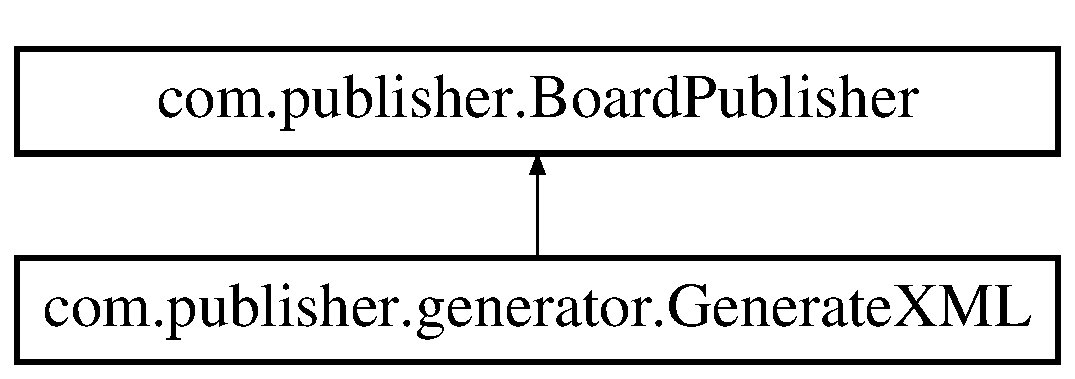
\includegraphics[height=2.000000cm]{db/dd9/interfacecom_1_1publisher_1_1BoardPublisher}
\end{center}
\end{figure}
\subsection*{Fonctions membres publiques}
\begin{DoxyCompactItemize}
\item 
void \hyperlink{interfacecom_1_1publisher_1_1BoardPublisher_a608aad61bbb4187737a5a6352d6e4454}{board\-Maker} ()
\end{DoxyCompactItemize}
\subsection*{Attributs publics statiques}
\begin{DoxyCompactItemize}
\item 
static final String \hyperlink{interfacecom_1_1publisher_1_1BoardPublisher_a4cc34fc55d558d4d567bb4835faca1cb}{W\-H\-I\-T\-E} = \char`\"{}white\char`\"{}
\item 
static final String \hyperlink{interfacecom_1_1publisher_1_1BoardPublisher_aba94dc86e361ca79b6837d7be045a9a8}{B\-L\-A\-C\-K} = \char`\"{}black\char`\"{}
\item 
static final String \hyperlink{interfacecom_1_1publisher_1_1BoardPublisher_aa1f69b7f88b84c429507c8e1a1a05dfc}{H\-U\-M\-A\-N} = \char`\"{}human\char`\"{}
\item 
static final String \hyperlink{interfacecom_1_1publisher_1_1BoardPublisher_a129aef59c73a473f569518604209f9a5}{M\-A\-C\-H\-I\-N\-E} = \char`\"{}machine\char`\"{}
\item 
static final String \hyperlink{interfacecom_1_1publisher_1_1BoardPublisher_a92afdb8fe43445ae26666c639e029947}{B\-O\-A\-R\-D\-\_\-\-P\-A\-R\-T} = \char`\"{}board\char`\"{}
\item 
static final String \hyperlink{interfacecom_1_1publisher_1_1BoardPublisher_a4284ddedaea2e3e014c275c71b630151}{I\-N\-I\-T\-\_\-\-P\-A\-R\-T} = \char`\"{}init\char`\"{}
\item 
static final String \hyperlink{interfacecom_1_1publisher_1_1BoardPublisher_adee2a9754672ab7fa9c7444670675652}{S\-I\-Z\-E\-\_\-\-P\-A\-R\-T} = \char`\"{}size\char`\"{}
\item 
static final String \hyperlink{interfacecom_1_1publisher_1_1BoardPublisher_a2b1aa577a5813b50376be3b43b673871}{X\-\_\-\-P\-A\-R\-T} = \char`\"{}x\char`\"{}
\item 
static final String \hyperlink{interfacecom_1_1publisher_1_1BoardPublisher_a9a0cac8873d240fbeac51b8b9d63c989}{Y\-\_\-\-P\-A\-R\-T} = \char`\"{}y\char`\"{}
\item 
static final String \hyperlink{interfacecom_1_1publisher_1_1BoardPublisher_a1b9e7130f674f96f073a47a31c6f7f7a}{C\-O\-L\-O\-R\-\_\-\-P\-A\-R\-T} = \char`\"{}c\char`\"{}
\item 
static final String \hyperlink{interfacecom_1_1publisher_1_1BoardPublisher_aa1c1d112ea8a987b5b6c75977b1c8f62}{P\-I\-E\-C\-E\-S\-\_\-\-P\-A\-R\-T} = \char`\"{}pieces\char`\"{}
\item 
static final String \hyperlink{interfacecom_1_1publisher_1_1BoardPublisher_a9f510b47f92ce1a0a4f716f63af1a226}{P\-I\-E\-C\-E\-\_\-\-P\-A\-R\-T} = \char`\"{}piece\char`\"{}
\item 
static final String \hyperlink{interfacecom_1_1publisher_1_1BoardPublisher_abbeefc71cd90ad0fec6ff50ab5cf2844}{P\-L\-A\-Y\-E\-R\-\_\-\-P\-A\-R\-T} = \char`\"{}player\char`\"{}
\item 
static final String \hyperlink{interfacecom_1_1publisher_1_1BoardPublisher_a2d0128b35b0dd2fd6e39c72600db5e5e}{P\-L\-A\-Y\-E\-R\-\_\-\-L\-O\-G\-I\-N\-\_\-\-P\-A\-R\-T} = \char`\"{}name\char`\"{}
\item 
static final String \hyperlink{interfacecom_1_1publisher_1_1BoardPublisher_a19fc43fcd0518ae4fda36b0ae8f5a5b5}{P\-L\-A\-Y\-E\-R\-\_\-\-C\-O\-L\-O\-R\-\_\-\-P\-A\-R\-T} = \char`\"{}rgb\char`\"{}
\item 
static final String \hyperlink{interfacecom_1_1publisher_1_1BoardPublisher_a46cc4c07629b28cb80562eb26e6ba203}{P\-L\-A\-Y\-E\-R\-\_\-\-T\-Y\-P\-E\-\_\-\-P\-A\-R\-T} = \char`\"{}type\char`\"{}
\item 
static final String \hyperlink{interfacecom_1_1publisher_1_1BoardPublisher_ada5e40ef43bea9a32144b7772ff68882}{P\-L\-A\-Y\-E\-R\-\_\-\-N\-U\-M\-B\-E\-R\-\_\-\-P\-A\-R\-T} = \char`\"{}num\char`\"{}
\item 
static final String \hyperlink{interfacecom_1_1publisher_1_1BoardPublisher_aae576f06d1b439ecdc67cf86b0a3ac00}{A\-I\-\_\-\-L\-E\-V\-E\-L\-\_\-\-P\-A\-R\-T} = \char`\"{}A\-I\-Level\char`\"{}
\item 
static final String \hyperlink{interfacecom_1_1publisher_1_1BoardPublisher_a70adf8b9c4d2855f48d1f8ba6e791dc4}{A\-I\-\_\-\-T\-H\-I\-N\-K\-I\-N\-G\-\_\-\-T\-I\-M\-E\-\_\-\-P\-A\-R\-T} = \char`\"{}A\-I\-Thinking\-Time\char`\"{}
\item 
static final String \hyperlink{interfacecom_1_1publisher_1_1BoardPublisher_a79a3b42afcb9fba37f70796768497b8c}{P\-L\-A\-Y\-E\-D\-\_\-\-P\-I\-E\-C\-E\-S\-\_\-\-P\-A\-R\-T} = \char`\"{}played\-Pcs\char`\"{}
\item 
static final String \hyperlink{interfacecom_1_1publisher_1_1BoardPublisher_a748ec30f1f7c5b9df00b87395e68804b}{H\-I\-S\-T\-O\-R\-Y\-\_\-\-P\-A\-R\-T} = \char`\"{}history\char`\"{}
\end{DoxyCompactItemize}


\subsection{Description détaillée}
Interface de gestion du module de génération de plateau pour Othello \begin{DoxyAuthor}{Auteur}

\begin{DoxyItemize}
\item Benjamin Letourneau
\end{DoxyItemize}
\end{DoxyAuthor}
\begin{DoxyVersion}{Version}
1.\-0 
\end{DoxyVersion}


\subsection{Documentation des fonctions membres}
\hypertarget{interfacecom_1_1publisher_1_1BoardPublisher_a608aad61bbb4187737a5a6352d6e4454}{\index{com\-::publisher\-::\-Board\-Publisher@{com\-::publisher\-::\-Board\-Publisher}!board\-Maker@{board\-Maker}}
\index{board\-Maker@{board\-Maker}!com::publisher::BoardPublisher@{com\-::publisher\-::\-Board\-Publisher}}
\subsubsection[{board\-Maker}]{\setlength{\rightskip}{0pt plus 5cm}void com.\-publisher.\-Board\-Publisher.\-board\-Maker (
\begin{DoxyParamCaption}
{}
\end{DoxyParamCaption}
)}}\label{interfacecom_1_1publisher_1_1BoardPublisher_a608aad61bbb4187737a5a6352d6e4454}
Methode permettant d'utiliser le module de génération d'othellier (plateau de jeu d'othello). 

Implémenté dans \hyperlink{classcom_1_1publisher_1_1generator_1_1GenerateXML_a0e0a8453dea04a5f36005f528bcf3d86}{com.\-publisher.\-generator.\-Generate\-X\-M\-L}.



\subsection{Documentation des données membres}
\hypertarget{interfacecom_1_1publisher_1_1BoardPublisher_aae576f06d1b439ecdc67cf86b0a3ac00}{\index{com\-::publisher\-::\-Board\-Publisher@{com\-::publisher\-::\-Board\-Publisher}!A\-I\-\_\-\-L\-E\-V\-E\-L\-\_\-\-P\-A\-R\-T@{A\-I\-\_\-\-L\-E\-V\-E\-L\-\_\-\-P\-A\-R\-T}}
\index{A\-I\-\_\-\-L\-E\-V\-E\-L\-\_\-\-P\-A\-R\-T@{A\-I\-\_\-\-L\-E\-V\-E\-L\-\_\-\-P\-A\-R\-T}!com::publisher::BoardPublisher@{com\-::publisher\-::\-Board\-Publisher}}
\subsubsection[{A\-I\-\_\-\-L\-E\-V\-E\-L\-\_\-\-P\-A\-R\-T}]{\setlength{\rightskip}{0pt plus 5cm}final String com.\-publisher.\-Board\-Publisher.\-A\-I\-\_\-\-L\-E\-V\-E\-L\-\_\-\-P\-A\-R\-T = \char`\"{}A\-I\-Level\char`\"{}\hspace{0.3cm}{\ttfamily [static]}}}\label{interfacecom_1_1publisher_1_1BoardPublisher_aae576f06d1b439ecdc67cf86b0a3ac00}
\hypertarget{interfacecom_1_1publisher_1_1BoardPublisher_a70adf8b9c4d2855f48d1f8ba6e791dc4}{\index{com\-::publisher\-::\-Board\-Publisher@{com\-::publisher\-::\-Board\-Publisher}!A\-I\-\_\-\-T\-H\-I\-N\-K\-I\-N\-G\-\_\-\-T\-I\-M\-E\-\_\-\-P\-A\-R\-T@{A\-I\-\_\-\-T\-H\-I\-N\-K\-I\-N\-G\-\_\-\-T\-I\-M\-E\-\_\-\-P\-A\-R\-T}}
\index{A\-I\-\_\-\-T\-H\-I\-N\-K\-I\-N\-G\-\_\-\-T\-I\-M\-E\-\_\-\-P\-A\-R\-T@{A\-I\-\_\-\-T\-H\-I\-N\-K\-I\-N\-G\-\_\-\-T\-I\-M\-E\-\_\-\-P\-A\-R\-T}!com::publisher::BoardPublisher@{com\-::publisher\-::\-Board\-Publisher}}
\subsubsection[{A\-I\-\_\-\-T\-H\-I\-N\-K\-I\-N\-G\-\_\-\-T\-I\-M\-E\-\_\-\-P\-A\-R\-T}]{\setlength{\rightskip}{0pt plus 5cm}final String com.\-publisher.\-Board\-Publisher.\-A\-I\-\_\-\-T\-H\-I\-N\-K\-I\-N\-G\-\_\-\-T\-I\-M\-E\-\_\-\-P\-A\-R\-T = \char`\"{}A\-I\-Thinking\-Time\char`\"{}\hspace{0.3cm}{\ttfamily [static]}}}\label{interfacecom_1_1publisher_1_1BoardPublisher_a70adf8b9c4d2855f48d1f8ba6e791dc4}
\hypertarget{interfacecom_1_1publisher_1_1BoardPublisher_aba94dc86e361ca79b6837d7be045a9a8}{\index{com\-::publisher\-::\-Board\-Publisher@{com\-::publisher\-::\-Board\-Publisher}!B\-L\-A\-C\-K@{B\-L\-A\-C\-K}}
\index{B\-L\-A\-C\-K@{B\-L\-A\-C\-K}!com::publisher::BoardPublisher@{com\-::publisher\-::\-Board\-Publisher}}
\subsubsection[{B\-L\-A\-C\-K}]{\setlength{\rightskip}{0pt plus 5cm}final String com.\-publisher.\-Board\-Publisher.\-B\-L\-A\-C\-K = \char`\"{}black\char`\"{}\hspace{0.3cm}{\ttfamily [static]}}}\label{interfacecom_1_1publisher_1_1BoardPublisher_aba94dc86e361ca79b6837d7be045a9a8}
\hypertarget{interfacecom_1_1publisher_1_1BoardPublisher_a92afdb8fe43445ae26666c639e029947}{\index{com\-::publisher\-::\-Board\-Publisher@{com\-::publisher\-::\-Board\-Publisher}!B\-O\-A\-R\-D\-\_\-\-P\-A\-R\-T@{B\-O\-A\-R\-D\-\_\-\-P\-A\-R\-T}}
\index{B\-O\-A\-R\-D\-\_\-\-P\-A\-R\-T@{B\-O\-A\-R\-D\-\_\-\-P\-A\-R\-T}!com::publisher::BoardPublisher@{com\-::publisher\-::\-Board\-Publisher}}
\subsubsection[{B\-O\-A\-R\-D\-\_\-\-P\-A\-R\-T}]{\setlength{\rightskip}{0pt plus 5cm}final String com.\-publisher.\-Board\-Publisher.\-B\-O\-A\-R\-D\-\_\-\-P\-A\-R\-T = \char`\"{}board\char`\"{}\hspace{0.3cm}{\ttfamily [static]}}}\label{interfacecom_1_1publisher_1_1BoardPublisher_a92afdb8fe43445ae26666c639e029947}
Constantes permettant de générer le fichier de sauvegarde. \hypertarget{interfacecom_1_1publisher_1_1BoardPublisher_a1b9e7130f674f96f073a47a31c6f7f7a}{\index{com\-::publisher\-::\-Board\-Publisher@{com\-::publisher\-::\-Board\-Publisher}!C\-O\-L\-O\-R\-\_\-\-P\-A\-R\-T@{C\-O\-L\-O\-R\-\_\-\-P\-A\-R\-T}}
\index{C\-O\-L\-O\-R\-\_\-\-P\-A\-R\-T@{C\-O\-L\-O\-R\-\_\-\-P\-A\-R\-T}!com::publisher::BoardPublisher@{com\-::publisher\-::\-Board\-Publisher}}
\subsubsection[{C\-O\-L\-O\-R\-\_\-\-P\-A\-R\-T}]{\setlength{\rightskip}{0pt plus 5cm}final String com.\-publisher.\-Board\-Publisher.\-C\-O\-L\-O\-R\-\_\-\-P\-A\-R\-T = \char`\"{}c\char`\"{}\hspace{0.3cm}{\ttfamily [static]}}}\label{interfacecom_1_1publisher_1_1BoardPublisher_a1b9e7130f674f96f073a47a31c6f7f7a}
\hypertarget{interfacecom_1_1publisher_1_1BoardPublisher_a748ec30f1f7c5b9df00b87395e68804b}{\index{com\-::publisher\-::\-Board\-Publisher@{com\-::publisher\-::\-Board\-Publisher}!H\-I\-S\-T\-O\-R\-Y\-\_\-\-P\-A\-R\-T@{H\-I\-S\-T\-O\-R\-Y\-\_\-\-P\-A\-R\-T}}
\index{H\-I\-S\-T\-O\-R\-Y\-\_\-\-P\-A\-R\-T@{H\-I\-S\-T\-O\-R\-Y\-\_\-\-P\-A\-R\-T}!com::publisher::BoardPublisher@{com\-::publisher\-::\-Board\-Publisher}}
\subsubsection[{H\-I\-S\-T\-O\-R\-Y\-\_\-\-P\-A\-R\-T}]{\setlength{\rightskip}{0pt plus 5cm}final String com.\-publisher.\-Board\-Publisher.\-H\-I\-S\-T\-O\-R\-Y\-\_\-\-P\-A\-R\-T = \char`\"{}history\char`\"{}\hspace{0.3cm}{\ttfamily [static]}}}\label{interfacecom_1_1publisher_1_1BoardPublisher_a748ec30f1f7c5b9df00b87395e68804b}
\hypertarget{interfacecom_1_1publisher_1_1BoardPublisher_aa1f69b7f88b84c429507c8e1a1a05dfc}{\index{com\-::publisher\-::\-Board\-Publisher@{com\-::publisher\-::\-Board\-Publisher}!H\-U\-M\-A\-N@{H\-U\-M\-A\-N}}
\index{H\-U\-M\-A\-N@{H\-U\-M\-A\-N}!com::publisher::BoardPublisher@{com\-::publisher\-::\-Board\-Publisher}}
\subsubsection[{H\-U\-M\-A\-N}]{\setlength{\rightskip}{0pt plus 5cm}final String com.\-publisher.\-Board\-Publisher.\-H\-U\-M\-A\-N = \char`\"{}human\char`\"{}\hspace{0.3cm}{\ttfamily [static]}}}\label{interfacecom_1_1publisher_1_1BoardPublisher_aa1f69b7f88b84c429507c8e1a1a05dfc}
Constante indiquant le type du joueur. \hypertarget{interfacecom_1_1publisher_1_1BoardPublisher_a4284ddedaea2e3e014c275c71b630151}{\index{com\-::publisher\-::\-Board\-Publisher@{com\-::publisher\-::\-Board\-Publisher}!I\-N\-I\-T\-\_\-\-P\-A\-R\-T@{I\-N\-I\-T\-\_\-\-P\-A\-R\-T}}
\index{I\-N\-I\-T\-\_\-\-P\-A\-R\-T@{I\-N\-I\-T\-\_\-\-P\-A\-R\-T}!com::publisher::BoardPublisher@{com\-::publisher\-::\-Board\-Publisher}}
\subsubsection[{I\-N\-I\-T\-\_\-\-P\-A\-R\-T}]{\setlength{\rightskip}{0pt plus 5cm}final String com.\-publisher.\-Board\-Publisher.\-I\-N\-I\-T\-\_\-\-P\-A\-R\-T = \char`\"{}init\char`\"{}\hspace{0.3cm}{\ttfamily [static]}}}\label{interfacecom_1_1publisher_1_1BoardPublisher_a4284ddedaea2e3e014c275c71b630151}
\hypertarget{interfacecom_1_1publisher_1_1BoardPublisher_a129aef59c73a473f569518604209f9a5}{\index{com\-::publisher\-::\-Board\-Publisher@{com\-::publisher\-::\-Board\-Publisher}!M\-A\-C\-H\-I\-N\-E@{M\-A\-C\-H\-I\-N\-E}}
\index{M\-A\-C\-H\-I\-N\-E@{M\-A\-C\-H\-I\-N\-E}!com::publisher::BoardPublisher@{com\-::publisher\-::\-Board\-Publisher}}
\subsubsection[{M\-A\-C\-H\-I\-N\-E}]{\setlength{\rightskip}{0pt plus 5cm}final String com.\-publisher.\-Board\-Publisher.\-M\-A\-C\-H\-I\-N\-E = \char`\"{}machine\char`\"{}\hspace{0.3cm}{\ttfamily [static]}}}\label{interfacecom_1_1publisher_1_1BoardPublisher_a129aef59c73a473f569518604209f9a5}
\hypertarget{interfacecom_1_1publisher_1_1BoardPublisher_a9f510b47f92ce1a0a4f716f63af1a226}{\index{com\-::publisher\-::\-Board\-Publisher@{com\-::publisher\-::\-Board\-Publisher}!P\-I\-E\-C\-E\-\_\-\-P\-A\-R\-T@{P\-I\-E\-C\-E\-\_\-\-P\-A\-R\-T}}
\index{P\-I\-E\-C\-E\-\_\-\-P\-A\-R\-T@{P\-I\-E\-C\-E\-\_\-\-P\-A\-R\-T}!com::publisher::BoardPublisher@{com\-::publisher\-::\-Board\-Publisher}}
\subsubsection[{P\-I\-E\-C\-E\-\_\-\-P\-A\-R\-T}]{\setlength{\rightskip}{0pt plus 5cm}final String com.\-publisher.\-Board\-Publisher.\-P\-I\-E\-C\-E\-\_\-\-P\-A\-R\-T = \char`\"{}piece\char`\"{}\hspace{0.3cm}{\ttfamily [static]}}}\label{interfacecom_1_1publisher_1_1BoardPublisher_a9f510b47f92ce1a0a4f716f63af1a226}
\hypertarget{interfacecom_1_1publisher_1_1BoardPublisher_aa1c1d112ea8a987b5b6c75977b1c8f62}{\index{com\-::publisher\-::\-Board\-Publisher@{com\-::publisher\-::\-Board\-Publisher}!P\-I\-E\-C\-E\-S\-\_\-\-P\-A\-R\-T@{P\-I\-E\-C\-E\-S\-\_\-\-P\-A\-R\-T}}
\index{P\-I\-E\-C\-E\-S\-\_\-\-P\-A\-R\-T@{P\-I\-E\-C\-E\-S\-\_\-\-P\-A\-R\-T}!com::publisher::BoardPublisher@{com\-::publisher\-::\-Board\-Publisher}}
\subsubsection[{P\-I\-E\-C\-E\-S\-\_\-\-P\-A\-R\-T}]{\setlength{\rightskip}{0pt plus 5cm}final String com.\-publisher.\-Board\-Publisher.\-P\-I\-E\-C\-E\-S\-\_\-\-P\-A\-R\-T = \char`\"{}pieces\char`\"{}\hspace{0.3cm}{\ttfamily [static]}}}\label{interfacecom_1_1publisher_1_1BoardPublisher_aa1c1d112ea8a987b5b6c75977b1c8f62}
\hypertarget{interfacecom_1_1publisher_1_1BoardPublisher_a79a3b42afcb9fba37f70796768497b8c}{\index{com\-::publisher\-::\-Board\-Publisher@{com\-::publisher\-::\-Board\-Publisher}!P\-L\-A\-Y\-E\-D\-\_\-\-P\-I\-E\-C\-E\-S\-\_\-\-P\-A\-R\-T@{P\-L\-A\-Y\-E\-D\-\_\-\-P\-I\-E\-C\-E\-S\-\_\-\-P\-A\-R\-T}}
\index{P\-L\-A\-Y\-E\-D\-\_\-\-P\-I\-E\-C\-E\-S\-\_\-\-P\-A\-R\-T@{P\-L\-A\-Y\-E\-D\-\_\-\-P\-I\-E\-C\-E\-S\-\_\-\-P\-A\-R\-T}!com::publisher::BoardPublisher@{com\-::publisher\-::\-Board\-Publisher}}
\subsubsection[{P\-L\-A\-Y\-E\-D\-\_\-\-P\-I\-E\-C\-E\-S\-\_\-\-P\-A\-R\-T}]{\setlength{\rightskip}{0pt plus 5cm}final String com.\-publisher.\-Board\-Publisher.\-P\-L\-A\-Y\-E\-D\-\_\-\-P\-I\-E\-C\-E\-S\-\_\-\-P\-A\-R\-T = \char`\"{}played\-Pcs\char`\"{}\hspace{0.3cm}{\ttfamily [static]}}}\label{interfacecom_1_1publisher_1_1BoardPublisher_a79a3b42afcb9fba37f70796768497b8c}
\hypertarget{interfacecom_1_1publisher_1_1BoardPublisher_a19fc43fcd0518ae4fda36b0ae8f5a5b5}{\index{com\-::publisher\-::\-Board\-Publisher@{com\-::publisher\-::\-Board\-Publisher}!P\-L\-A\-Y\-E\-R\-\_\-\-C\-O\-L\-O\-R\-\_\-\-P\-A\-R\-T@{P\-L\-A\-Y\-E\-R\-\_\-\-C\-O\-L\-O\-R\-\_\-\-P\-A\-R\-T}}
\index{P\-L\-A\-Y\-E\-R\-\_\-\-C\-O\-L\-O\-R\-\_\-\-P\-A\-R\-T@{P\-L\-A\-Y\-E\-R\-\_\-\-C\-O\-L\-O\-R\-\_\-\-P\-A\-R\-T}!com::publisher::BoardPublisher@{com\-::publisher\-::\-Board\-Publisher}}
\subsubsection[{P\-L\-A\-Y\-E\-R\-\_\-\-C\-O\-L\-O\-R\-\_\-\-P\-A\-R\-T}]{\setlength{\rightskip}{0pt plus 5cm}final String com.\-publisher.\-Board\-Publisher.\-P\-L\-A\-Y\-E\-R\-\_\-\-C\-O\-L\-O\-R\-\_\-\-P\-A\-R\-T = \char`\"{}rgb\char`\"{}\hspace{0.3cm}{\ttfamily [static]}}}\label{interfacecom_1_1publisher_1_1BoardPublisher_a19fc43fcd0518ae4fda36b0ae8f5a5b5}
\hypertarget{interfacecom_1_1publisher_1_1BoardPublisher_a2d0128b35b0dd2fd6e39c72600db5e5e}{\index{com\-::publisher\-::\-Board\-Publisher@{com\-::publisher\-::\-Board\-Publisher}!P\-L\-A\-Y\-E\-R\-\_\-\-L\-O\-G\-I\-N\-\_\-\-P\-A\-R\-T@{P\-L\-A\-Y\-E\-R\-\_\-\-L\-O\-G\-I\-N\-\_\-\-P\-A\-R\-T}}
\index{P\-L\-A\-Y\-E\-R\-\_\-\-L\-O\-G\-I\-N\-\_\-\-P\-A\-R\-T@{P\-L\-A\-Y\-E\-R\-\_\-\-L\-O\-G\-I\-N\-\_\-\-P\-A\-R\-T}!com::publisher::BoardPublisher@{com\-::publisher\-::\-Board\-Publisher}}
\subsubsection[{P\-L\-A\-Y\-E\-R\-\_\-\-L\-O\-G\-I\-N\-\_\-\-P\-A\-R\-T}]{\setlength{\rightskip}{0pt plus 5cm}final String com.\-publisher.\-Board\-Publisher.\-P\-L\-A\-Y\-E\-R\-\_\-\-L\-O\-G\-I\-N\-\_\-\-P\-A\-R\-T = \char`\"{}name\char`\"{}\hspace{0.3cm}{\ttfamily [static]}}}\label{interfacecom_1_1publisher_1_1BoardPublisher_a2d0128b35b0dd2fd6e39c72600db5e5e}
\hypertarget{interfacecom_1_1publisher_1_1BoardPublisher_ada5e40ef43bea9a32144b7772ff68882}{\index{com\-::publisher\-::\-Board\-Publisher@{com\-::publisher\-::\-Board\-Publisher}!P\-L\-A\-Y\-E\-R\-\_\-\-N\-U\-M\-B\-E\-R\-\_\-\-P\-A\-R\-T@{P\-L\-A\-Y\-E\-R\-\_\-\-N\-U\-M\-B\-E\-R\-\_\-\-P\-A\-R\-T}}
\index{P\-L\-A\-Y\-E\-R\-\_\-\-N\-U\-M\-B\-E\-R\-\_\-\-P\-A\-R\-T@{P\-L\-A\-Y\-E\-R\-\_\-\-N\-U\-M\-B\-E\-R\-\_\-\-P\-A\-R\-T}!com::publisher::BoardPublisher@{com\-::publisher\-::\-Board\-Publisher}}
\subsubsection[{P\-L\-A\-Y\-E\-R\-\_\-\-N\-U\-M\-B\-E\-R\-\_\-\-P\-A\-R\-T}]{\setlength{\rightskip}{0pt plus 5cm}final String com.\-publisher.\-Board\-Publisher.\-P\-L\-A\-Y\-E\-R\-\_\-\-N\-U\-M\-B\-E\-R\-\_\-\-P\-A\-R\-T = \char`\"{}num\char`\"{}\hspace{0.3cm}{\ttfamily [static]}}}\label{interfacecom_1_1publisher_1_1BoardPublisher_ada5e40ef43bea9a32144b7772ff68882}
\hypertarget{interfacecom_1_1publisher_1_1BoardPublisher_abbeefc71cd90ad0fec6ff50ab5cf2844}{\index{com\-::publisher\-::\-Board\-Publisher@{com\-::publisher\-::\-Board\-Publisher}!P\-L\-A\-Y\-E\-R\-\_\-\-P\-A\-R\-T@{P\-L\-A\-Y\-E\-R\-\_\-\-P\-A\-R\-T}}
\index{P\-L\-A\-Y\-E\-R\-\_\-\-P\-A\-R\-T@{P\-L\-A\-Y\-E\-R\-\_\-\-P\-A\-R\-T}!com::publisher::BoardPublisher@{com\-::publisher\-::\-Board\-Publisher}}
\subsubsection[{P\-L\-A\-Y\-E\-R\-\_\-\-P\-A\-R\-T}]{\setlength{\rightskip}{0pt plus 5cm}final String com.\-publisher.\-Board\-Publisher.\-P\-L\-A\-Y\-E\-R\-\_\-\-P\-A\-R\-T = \char`\"{}player\char`\"{}\hspace{0.3cm}{\ttfamily [static]}}}\label{interfacecom_1_1publisher_1_1BoardPublisher_abbeefc71cd90ad0fec6ff50ab5cf2844}
\hypertarget{interfacecom_1_1publisher_1_1BoardPublisher_a46cc4c07629b28cb80562eb26e6ba203}{\index{com\-::publisher\-::\-Board\-Publisher@{com\-::publisher\-::\-Board\-Publisher}!P\-L\-A\-Y\-E\-R\-\_\-\-T\-Y\-P\-E\-\_\-\-P\-A\-R\-T@{P\-L\-A\-Y\-E\-R\-\_\-\-T\-Y\-P\-E\-\_\-\-P\-A\-R\-T}}
\index{P\-L\-A\-Y\-E\-R\-\_\-\-T\-Y\-P\-E\-\_\-\-P\-A\-R\-T@{P\-L\-A\-Y\-E\-R\-\_\-\-T\-Y\-P\-E\-\_\-\-P\-A\-R\-T}!com::publisher::BoardPublisher@{com\-::publisher\-::\-Board\-Publisher}}
\subsubsection[{P\-L\-A\-Y\-E\-R\-\_\-\-T\-Y\-P\-E\-\_\-\-P\-A\-R\-T}]{\setlength{\rightskip}{0pt plus 5cm}final String com.\-publisher.\-Board\-Publisher.\-P\-L\-A\-Y\-E\-R\-\_\-\-T\-Y\-P\-E\-\_\-\-P\-A\-R\-T = \char`\"{}type\char`\"{}\hspace{0.3cm}{\ttfamily [static]}}}\label{interfacecom_1_1publisher_1_1BoardPublisher_a46cc4c07629b28cb80562eb26e6ba203}
\hypertarget{interfacecom_1_1publisher_1_1BoardPublisher_adee2a9754672ab7fa9c7444670675652}{\index{com\-::publisher\-::\-Board\-Publisher@{com\-::publisher\-::\-Board\-Publisher}!S\-I\-Z\-E\-\_\-\-P\-A\-R\-T@{S\-I\-Z\-E\-\_\-\-P\-A\-R\-T}}
\index{S\-I\-Z\-E\-\_\-\-P\-A\-R\-T@{S\-I\-Z\-E\-\_\-\-P\-A\-R\-T}!com::publisher::BoardPublisher@{com\-::publisher\-::\-Board\-Publisher}}
\subsubsection[{S\-I\-Z\-E\-\_\-\-P\-A\-R\-T}]{\setlength{\rightskip}{0pt plus 5cm}final String com.\-publisher.\-Board\-Publisher.\-S\-I\-Z\-E\-\_\-\-P\-A\-R\-T = \char`\"{}size\char`\"{}\hspace{0.3cm}{\ttfamily [static]}}}\label{interfacecom_1_1publisher_1_1BoardPublisher_adee2a9754672ab7fa9c7444670675652}
\hypertarget{interfacecom_1_1publisher_1_1BoardPublisher_a4cc34fc55d558d4d567bb4835faca1cb}{\index{com\-::publisher\-::\-Board\-Publisher@{com\-::publisher\-::\-Board\-Publisher}!W\-H\-I\-T\-E@{W\-H\-I\-T\-E}}
\index{W\-H\-I\-T\-E@{W\-H\-I\-T\-E}!com::publisher::BoardPublisher@{com\-::publisher\-::\-Board\-Publisher}}
\subsubsection[{W\-H\-I\-T\-E}]{\setlength{\rightskip}{0pt plus 5cm}final String com.\-publisher.\-Board\-Publisher.\-W\-H\-I\-T\-E = \char`\"{}white\char`\"{}\hspace{0.3cm}{\ttfamily [static]}}}\label{interfacecom_1_1publisher_1_1BoardPublisher_a4cc34fc55d558d4d567bb4835faca1cb}
Constantes indiquant la couleur du joueur. \hypertarget{interfacecom_1_1publisher_1_1BoardPublisher_a2b1aa577a5813b50376be3b43b673871}{\index{com\-::publisher\-::\-Board\-Publisher@{com\-::publisher\-::\-Board\-Publisher}!X\-\_\-\-P\-A\-R\-T@{X\-\_\-\-P\-A\-R\-T}}
\index{X\-\_\-\-P\-A\-R\-T@{X\-\_\-\-P\-A\-R\-T}!com::publisher::BoardPublisher@{com\-::publisher\-::\-Board\-Publisher}}
\subsubsection[{X\-\_\-\-P\-A\-R\-T}]{\setlength{\rightskip}{0pt plus 5cm}final String com.\-publisher.\-Board\-Publisher.\-X\-\_\-\-P\-A\-R\-T = \char`\"{}x\char`\"{}\hspace{0.3cm}{\ttfamily [static]}}}\label{interfacecom_1_1publisher_1_1BoardPublisher_a2b1aa577a5813b50376be3b43b673871}
\hypertarget{interfacecom_1_1publisher_1_1BoardPublisher_a9a0cac8873d240fbeac51b8b9d63c989}{\index{com\-::publisher\-::\-Board\-Publisher@{com\-::publisher\-::\-Board\-Publisher}!Y\-\_\-\-P\-A\-R\-T@{Y\-\_\-\-P\-A\-R\-T}}
\index{Y\-\_\-\-P\-A\-R\-T@{Y\-\_\-\-P\-A\-R\-T}!com::publisher::BoardPublisher@{com\-::publisher\-::\-Board\-Publisher}}
\subsubsection[{Y\-\_\-\-P\-A\-R\-T}]{\setlength{\rightskip}{0pt plus 5cm}final String com.\-publisher.\-Board\-Publisher.\-Y\-\_\-\-P\-A\-R\-T = \char`\"{}y\char`\"{}\hspace{0.3cm}{\ttfamily [static]}}}\label{interfacecom_1_1publisher_1_1BoardPublisher_a9a0cac8873d240fbeac51b8b9d63c989}


La documentation de cette interface a été générée à partir du fichier suivant \-:\begin{DoxyCompactItemize}
\item 
\hyperlink{BoardPublisher_8java}{Board\-Publisher.\-java}\end{DoxyCompactItemize}

\hypertarget{classcom_1_1publisher_1_1utils_1_1BPHandlerException}{\section{Référence de la classe com.\-publisher.\-utils.\-B\-P\-Handler\-Exception}
\label{classcom_1_1publisher_1_1utils_1_1BPHandlerException}\index{com.\-publisher.\-utils.\-B\-P\-Handler\-Exception@{com.\-publisher.\-utils.\-B\-P\-Handler\-Exception}}
}
Graphe d'héritage de com.\-publisher.\-utils.\-B\-P\-Handler\-Exception\-:\begin{figure}[H]
\begin{center}
\leavevmode
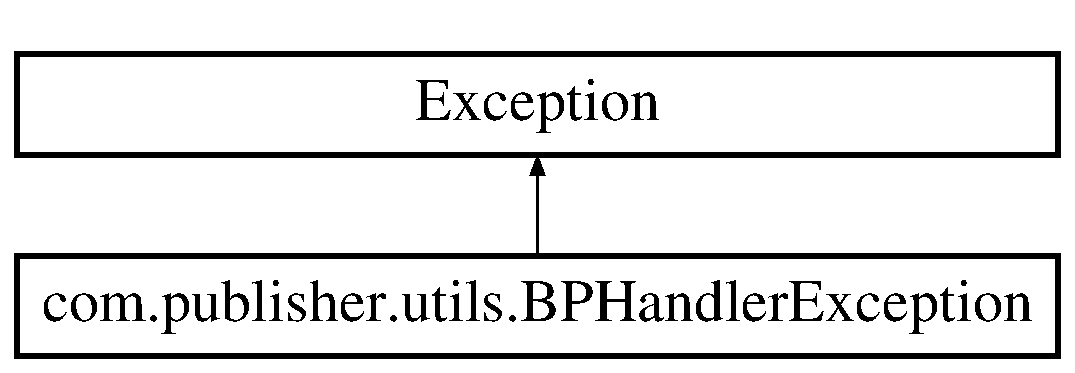
\includegraphics[height=2.000000cm]{d3/db2/classcom_1_1publisher_1_1utils_1_1BPHandlerException}
\end{center}
\end{figure}
\subsection*{Fonctions membres publiques}
\begin{DoxyCompactItemize}
\item 
\hyperlink{classcom_1_1publisher_1_1utils_1_1BPHandlerException_a29621bd49601c323ae814695e2592fd6}{B\-P\-Handler\-Exception} (int \hyperlink{classcom_1_1publisher_1_1utils_1_1BPHandlerException_a22187f6ed53004154eead03978409a11}{error})
\item 
\hyperlink{classcom_1_1publisher_1_1utils_1_1BPHandlerException_a3c306310302b1e4dcad1cdda127cf119}{B\-P\-Handler\-Exception} (int \hyperlink{classcom_1_1publisher_1_1utils_1_1BPHandlerException_a22187f6ed53004154eead03978409a11}{error}, String \hyperlink{classcom_1_1publisher_1_1utils_1_1BPHandlerException_ad64b758d099e991b5b86d489b56e582b}{message})
\item 
String \hyperlink{classcom_1_1publisher_1_1utils_1_1BPHandlerException_aa1d1deb769bfcb3faafd48ad754764fc}{get\-Message} ()
\end{DoxyCompactItemize}
\subsection*{Attributs publics statiques}
\begin{DoxyCompactItemize}
\item 
static final int \hyperlink{classcom_1_1publisher_1_1utils_1_1BPHandlerException_a3aad32cd8b00b8e2935e58f8cac14a0f}{E\-R\-R\-O\-R} = 0
\end{DoxyCompactItemize}
\subsection*{Attributs privés}
\begin{DoxyCompactItemize}
\item 
int \hyperlink{classcom_1_1publisher_1_1utils_1_1BPHandlerException_a22187f6ed53004154eead03978409a11}{error}
\item 
String \hyperlink{classcom_1_1publisher_1_1utils_1_1BPHandlerException_ad64b758d099e991b5b86d489b56e582b}{message}
\end{DoxyCompactItemize}


\subsection{Description détaillée}
Classe de gestion d'exceptions dans le \hyperlink{interfacecom_1_1publisher_1_1BoardPublisher}{Board\-Publisher}. \begin{DoxyAuthor}{Auteur}

\begin{DoxyItemize}
\item Benjamin Letourneau 
\end{DoxyItemize}
\end{DoxyAuthor}
\begin{DoxyVersion}{Version}
1.\-0 
\end{DoxyVersion}


\subsection{Documentation des constructeurs et destructeur}
\hypertarget{classcom_1_1publisher_1_1utils_1_1BPHandlerException_a29621bd49601c323ae814695e2592fd6}{\index{com\-::publisher\-::utils\-::\-B\-P\-Handler\-Exception@{com\-::publisher\-::utils\-::\-B\-P\-Handler\-Exception}!B\-P\-Handler\-Exception@{B\-P\-Handler\-Exception}}
\index{B\-P\-Handler\-Exception@{B\-P\-Handler\-Exception}!com::publisher::utils::BPHandlerException@{com\-::publisher\-::utils\-::\-B\-P\-Handler\-Exception}}
\subsubsection[{B\-P\-Handler\-Exception}]{\setlength{\rightskip}{0pt plus 5cm}com.\-publisher.\-utils.\-B\-P\-Handler\-Exception.\-B\-P\-Handler\-Exception (
\begin{DoxyParamCaption}
\item[{int}]{error}
\end{DoxyParamCaption}
)}}\label{classcom_1_1publisher_1_1utils_1_1BPHandlerException_a29621bd49601c323ae814695e2592fd6}
Constructeur de classe. 
\begin{DoxyParams}{Paramètres}
{\em error} & \-: int, numéro de l'erreur. \\
\hline
\end{DoxyParams}
\hypertarget{classcom_1_1publisher_1_1utils_1_1BPHandlerException_a3c306310302b1e4dcad1cdda127cf119}{\index{com\-::publisher\-::utils\-::\-B\-P\-Handler\-Exception@{com\-::publisher\-::utils\-::\-B\-P\-Handler\-Exception}!B\-P\-Handler\-Exception@{B\-P\-Handler\-Exception}}
\index{B\-P\-Handler\-Exception@{B\-P\-Handler\-Exception}!com::publisher::utils::BPHandlerException@{com\-::publisher\-::utils\-::\-B\-P\-Handler\-Exception}}
\subsubsection[{B\-P\-Handler\-Exception}]{\setlength{\rightskip}{0pt plus 5cm}com.\-publisher.\-utils.\-B\-P\-Handler\-Exception.\-B\-P\-Handler\-Exception (
\begin{DoxyParamCaption}
\item[{int}]{error, }
\item[{String}]{message}
\end{DoxyParamCaption}
)}}\label{classcom_1_1publisher_1_1utils_1_1BPHandlerException_a3c306310302b1e4dcad1cdda127cf119}
Constructeur de classe. 
\begin{DoxyParams}{Paramètres}
{\em error} & \-: int, numéro de l'erreur. \\
\hline
{\em message} & \-: String, message complémentaire au message de base de l'erreur. \\
\hline
\end{DoxyParams}


\subsection{Documentation des fonctions membres}
\hypertarget{classcom_1_1publisher_1_1utils_1_1BPHandlerException_aa1d1deb769bfcb3faafd48ad754764fc}{\index{com\-::publisher\-::utils\-::\-B\-P\-Handler\-Exception@{com\-::publisher\-::utils\-::\-B\-P\-Handler\-Exception}!get\-Message@{get\-Message}}
\index{get\-Message@{get\-Message}!com::publisher::utils::BPHandlerException@{com\-::publisher\-::utils\-::\-B\-P\-Handler\-Exception}}
\subsubsection[{get\-Message}]{\setlength{\rightskip}{0pt plus 5cm}String com.\-publisher.\-utils.\-B\-P\-Handler\-Exception.\-get\-Message (
\begin{DoxyParamCaption}
{}
\end{DoxyParamCaption}
)}}\label{classcom_1_1publisher_1_1utils_1_1BPHandlerException_aa1d1deb769bfcb3faafd48ad754764fc}
Accesseur (lecture) sur le message d'erreur. 

\subsection{Documentation des données membres}
\hypertarget{classcom_1_1publisher_1_1utils_1_1BPHandlerException_a3aad32cd8b00b8e2935e58f8cac14a0f}{\index{com\-::publisher\-::utils\-::\-B\-P\-Handler\-Exception@{com\-::publisher\-::utils\-::\-B\-P\-Handler\-Exception}!E\-R\-R\-O\-R@{E\-R\-R\-O\-R}}
\index{E\-R\-R\-O\-R@{E\-R\-R\-O\-R}!com::publisher::utils::BPHandlerException@{com\-::publisher\-::utils\-::\-B\-P\-Handler\-Exception}}
\subsubsection[{E\-R\-R\-O\-R}]{\setlength{\rightskip}{0pt plus 5cm}final int com.\-publisher.\-utils.\-B\-P\-Handler\-Exception.\-E\-R\-R\-O\-R = 0\hspace{0.3cm}{\ttfamily [static]}}}\label{classcom_1_1publisher_1_1utils_1_1BPHandlerException_a3aad32cd8b00b8e2935e58f8cac14a0f}
Constantes d'erreurs \hypertarget{classcom_1_1publisher_1_1utils_1_1BPHandlerException_a22187f6ed53004154eead03978409a11}{\index{com\-::publisher\-::utils\-::\-B\-P\-Handler\-Exception@{com\-::publisher\-::utils\-::\-B\-P\-Handler\-Exception}!error@{error}}
\index{error@{error}!com::publisher::utils::BPHandlerException@{com\-::publisher\-::utils\-::\-B\-P\-Handler\-Exception}}
\subsubsection[{error}]{\setlength{\rightskip}{0pt plus 5cm}int com.\-publisher.\-utils.\-B\-P\-Handler\-Exception.\-error\hspace{0.3cm}{\ttfamily [private]}}}\label{classcom_1_1publisher_1_1utils_1_1BPHandlerException_a22187f6ed53004154eead03978409a11}
Permet de stocker la constante correspondant à l'erreur réccupérée. \hypertarget{classcom_1_1publisher_1_1utils_1_1BPHandlerException_ad64b758d099e991b5b86d489b56e582b}{\index{com\-::publisher\-::utils\-::\-B\-P\-Handler\-Exception@{com\-::publisher\-::utils\-::\-B\-P\-Handler\-Exception}!message@{message}}
\index{message@{message}!com::publisher::utils::BPHandlerException@{com\-::publisher\-::utils\-::\-B\-P\-Handler\-Exception}}
\subsubsection[{message}]{\setlength{\rightskip}{0pt plus 5cm}String com.\-publisher.\-utils.\-B\-P\-Handler\-Exception.\-message\hspace{0.3cm}{\ttfamily [private]}}}\label{classcom_1_1publisher_1_1utils_1_1BPHandlerException_ad64b758d099e991b5b86d489b56e582b}
Permet de stocker un message complémentaire au message basique de l'erreur. 

La documentation de cette classe a été générée à partir du fichier suivant \-:\begin{DoxyCompactItemize}
\item 
\hyperlink{BPHandlerException_8java}{B\-P\-Handler\-Exception.\-java}\end{DoxyCompactItemize}

\hypertarget{classcom_1_1publisher_1_1generator_1_1GenerateXML}{\section{Référence de la classe com.\-publisher.\-generator.\-Generate\-X\-M\-L}
\label{classcom_1_1publisher_1_1generator_1_1GenerateXML}\index{com.\-publisher.\-generator.\-Generate\-X\-M\-L@{com.\-publisher.\-generator.\-Generate\-X\-M\-L}}
}
Graphe d'héritage de com.\-publisher.\-generator.\-Generate\-X\-M\-L\-:\begin{figure}[H]
\begin{center}
\leavevmode
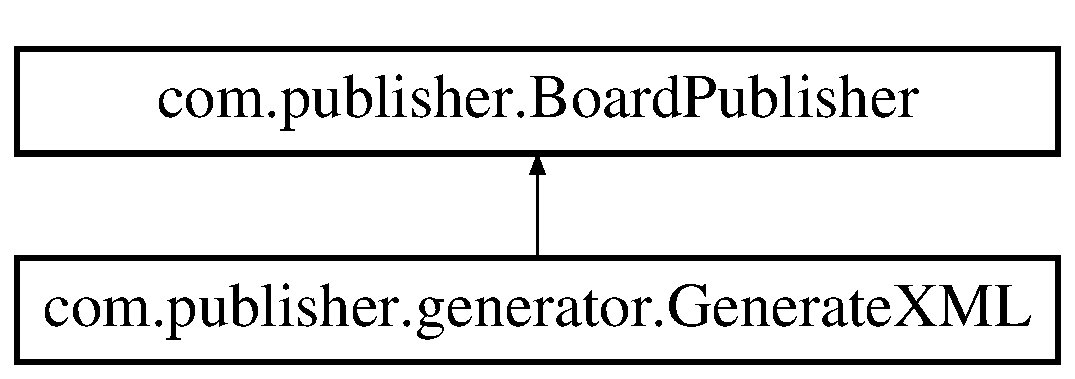
\includegraphics[height=2.000000cm]{d0/d88/classcom_1_1publisher_1_1generator_1_1GenerateXML}
\end{center}
\end{figure}
\subsection*{Fonctions membres publiques}
\begin{DoxyCompactItemize}
\item 
\hyperlink{classcom_1_1publisher_1_1generator_1_1GenerateXML_a0207e8c80c3243f24632232302a0b24c}{Generate\-X\-M\-L} ()
\item 
void \hyperlink{classcom_1_1publisher_1_1generator_1_1GenerateXML_a0e0a8453dea04a5f36005f528bcf3d86}{board\-Maker} ()
\item 
String \hyperlink{classcom_1_1publisher_1_1generator_1_1GenerateXML_a79351744ec4dbfd5aecc3a44626727c4}{to\-String} ()
\end{DoxyCompactItemize}
\subsection*{Fonctions membres privées}
\begin{DoxyCompactItemize}
\item 
Element \hyperlink{classcom_1_1publisher_1_1generator_1_1GenerateXML_ae3f30340ab6223aad945f96dfde40db8}{board\-Size\-In\-X\-M\-L} ()
\item 
Element \hyperlink{classcom_1_1publisher_1_1generator_1_1GenerateXML_a3a080523195e34489a684e33984448e8}{board\-Pieces\-In\-X\-M\-L} (String part)
\item 
Element \hyperlink{classcom_1_1publisher_1_1generator_1_1GenerateXML_aecfba9f11b369d214fe3ab1aed529bc5}{board\-Piece\-At\-In\-X\-M\-L} (int i, int j)
\item 
Element \hyperlink{classcom_1_1publisher_1_1generator_1_1GenerateXML_aca0e920a2c2064e744e501bdf66de93b}{player\-In\-X\-M\-L} (\hyperlink{classcom_1_1publisher_1_1Player}{Player} p)
\end{DoxyCompactItemize}
\subsection*{Attributs privés}
\begin{DoxyCompactItemize}
\item 
Element \hyperlink{classcom_1_1publisher_1_1generator_1_1GenerateXML_a700b8738d323998d4edcc17903ab1730}{root}
\item 
org.\-jdom2.\-Document \hyperlink{classcom_1_1publisher_1_1generator_1_1GenerateXML_a3eff314e550f7477f25d1c1624719f21}{save\-Doc}
\item 
\hyperlink{classcom_1_1publisher_1_1Board}{Board} \hyperlink{classcom_1_1publisher_1_1generator_1_1GenerateXML_afd9f81fe09deb4a51d4ddab0e52e5de9}{board}
\end{DoxyCompactItemize}
\subsection*{Membres hérités additionnels}


\subsection{Description détaillée}
Classe permettant de générer le nouvel Othellier formaté en X\-M\-L. \begin{DoxyAuthor}{Auteur}

\begin{DoxyItemize}
\item Benjamin Letourneau 
\end{DoxyItemize}
\end{DoxyAuthor}
\begin{DoxyVersion}{Version}
1.\-0 
\end{DoxyVersion}


\subsection{Documentation des constructeurs et destructeur}
\hypertarget{classcom_1_1publisher_1_1generator_1_1GenerateXML_a0207e8c80c3243f24632232302a0b24c}{\index{com\-::publisher\-::generator\-::\-Generate\-X\-M\-L@{com\-::publisher\-::generator\-::\-Generate\-X\-M\-L}!Generate\-X\-M\-L@{Generate\-X\-M\-L}}
\index{Generate\-X\-M\-L@{Generate\-X\-M\-L}!com::publisher::generator::GenerateXML@{com\-::publisher\-::generator\-::\-Generate\-X\-M\-L}}
\subsubsection[{Generate\-X\-M\-L}]{\setlength{\rightskip}{0pt plus 5cm}com.\-publisher.\-generator.\-Generate\-X\-M\-L.\-Generate\-X\-M\-L (
\begin{DoxyParamCaption}
{}
\end{DoxyParamCaption}
)}}\label{classcom_1_1publisher_1_1generator_1_1GenerateXML_a0207e8c80c3243f24632232302a0b24c}
Constructeur de classe. 

\subsection{Documentation des fonctions membres}
\hypertarget{classcom_1_1publisher_1_1generator_1_1GenerateXML_a0e0a8453dea04a5f36005f528bcf3d86}{\index{com\-::publisher\-::generator\-::\-Generate\-X\-M\-L@{com\-::publisher\-::generator\-::\-Generate\-X\-M\-L}!board\-Maker@{board\-Maker}}
\index{board\-Maker@{board\-Maker}!com::publisher::generator::GenerateXML@{com\-::publisher\-::generator\-::\-Generate\-X\-M\-L}}
\subsubsection[{board\-Maker}]{\setlength{\rightskip}{0pt plus 5cm}void com.\-publisher.\-generator.\-Generate\-X\-M\-L.\-board\-Maker (
\begin{DoxyParamCaption}
{}
\end{DoxyParamCaption}
)}}\label{classcom_1_1publisher_1_1generator_1_1GenerateXML_a0e0a8453dea04a5f36005f528bcf3d86}
Methode permettant d'utiliser le module de génération d'othellier (plateau de jeu d'othello). 

Implémente \hyperlink{interfacecom_1_1publisher_1_1BoardPublisher_a608aad61bbb4187737a5a6352d6e4454}{com.\-publisher.\-Board\-Publisher}.

\hypertarget{classcom_1_1publisher_1_1generator_1_1GenerateXML_aecfba9f11b369d214fe3ab1aed529bc5}{\index{com\-::publisher\-::generator\-::\-Generate\-X\-M\-L@{com\-::publisher\-::generator\-::\-Generate\-X\-M\-L}!board\-Piece\-At\-In\-X\-M\-L@{board\-Piece\-At\-In\-X\-M\-L}}
\index{board\-Piece\-At\-In\-X\-M\-L@{board\-Piece\-At\-In\-X\-M\-L}!com::publisher::generator::GenerateXML@{com\-::publisher\-::generator\-::\-Generate\-X\-M\-L}}
\subsubsection[{board\-Piece\-At\-In\-X\-M\-L}]{\setlength{\rightskip}{0pt plus 5cm}Element com.\-publisher.\-generator.\-Generate\-X\-M\-L.\-board\-Piece\-At\-In\-X\-M\-L (
\begin{DoxyParamCaption}
\item[{int}]{i, }
\item[{int}]{j}
\end{DoxyParamCaption}
)\hspace{0.3cm}{\ttfamily [private]}}}\label{classcom_1_1publisher_1_1generator_1_1GenerateXML_aecfba9f11b369d214fe3ab1aed529bc5}
Methode récupérant une pièce de l'Othellier en fonction des positions passés en paramètre. Attention il faut être sur que la couleur ne soit pas 0 car 0 correspond à une place vide dans l'Othellier. 
\begin{DoxyParams}{Paramètres}
{\em i} & \-: int, coordonnée de la pièce à réccupérer suivant l'axe des abscisses de l'Othellier. \\
\hline
{\em j} & \-: int, coordonnée de la pièce à réccupérer suivant l'axe des ordonnées de l'Othellier. \\
\hline
\end{DoxyParams}
\begin{DoxyReturn}{Renvoie}
Element \-: La pièce en X\-M\-L. 
\end{DoxyReturn}
\hypertarget{classcom_1_1publisher_1_1generator_1_1GenerateXML_a3a080523195e34489a684e33984448e8}{\index{com\-::publisher\-::generator\-::\-Generate\-X\-M\-L@{com\-::publisher\-::generator\-::\-Generate\-X\-M\-L}!board\-Pieces\-In\-X\-M\-L@{board\-Pieces\-In\-X\-M\-L}}
\index{board\-Pieces\-In\-X\-M\-L@{board\-Pieces\-In\-X\-M\-L}!com::publisher::generator::GenerateXML@{com\-::publisher\-::generator\-::\-Generate\-X\-M\-L}}
\subsubsection[{board\-Pieces\-In\-X\-M\-L}]{\setlength{\rightskip}{0pt plus 5cm}Element com.\-publisher.\-generator.\-Generate\-X\-M\-L.\-board\-Pieces\-In\-X\-M\-L (
\begin{DoxyParamCaption}
\item[{String}]{part}
\end{DoxyParamCaption}
)\hspace{0.3cm}{\ttfamily [private]}}}\label{classcom_1_1publisher_1_1generator_1_1GenerateXML_a3a080523195e34489a684e33984448e8}
Methode récupérant les pièces de l'Othellier afin de générer le X\-M\-L associé. \begin{DoxyReturn}{Renvoie}
Element \-: Les pièces en X\-M\-L. 
\end{DoxyReturn}
\hypertarget{classcom_1_1publisher_1_1generator_1_1GenerateXML_ae3f30340ab6223aad945f96dfde40db8}{\index{com\-::publisher\-::generator\-::\-Generate\-X\-M\-L@{com\-::publisher\-::generator\-::\-Generate\-X\-M\-L}!board\-Size\-In\-X\-M\-L@{board\-Size\-In\-X\-M\-L}}
\index{board\-Size\-In\-X\-M\-L@{board\-Size\-In\-X\-M\-L}!com::publisher::generator::GenerateXML@{com\-::publisher\-::generator\-::\-Generate\-X\-M\-L}}
\subsubsection[{board\-Size\-In\-X\-M\-L}]{\setlength{\rightskip}{0pt plus 5cm}Element com.\-publisher.\-generator.\-Generate\-X\-M\-L.\-board\-Size\-In\-X\-M\-L (
\begin{DoxyParamCaption}
{}
\end{DoxyParamCaption}
)\hspace{0.3cm}{\ttfamily [private]}}}\label{classcom_1_1publisher_1_1generator_1_1GenerateXML_ae3f30340ab6223aad945f96dfde40db8}
Methode récupérant la taille de l'Othellier et le formate en X\-M\-L. \begin{DoxyReturn}{Renvoie}
Element, la taille de l'Othellier en X\-M\-L. 
\end{DoxyReturn}
\hypertarget{classcom_1_1publisher_1_1generator_1_1GenerateXML_aca0e920a2c2064e744e501bdf66de93b}{\index{com\-::publisher\-::generator\-::\-Generate\-X\-M\-L@{com\-::publisher\-::generator\-::\-Generate\-X\-M\-L}!player\-In\-X\-M\-L@{player\-In\-X\-M\-L}}
\index{player\-In\-X\-M\-L@{player\-In\-X\-M\-L}!com::publisher::generator::GenerateXML@{com\-::publisher\-::generator\-::\-Generate\-X\-M\-L}}
\subsubsection[{player\-In\-X\-M\-L}]{\setlength{\rightskip}{0pt plus 5cm}Element com.\-publisher.\-generator.\-Generate\-X\-M\-L.\-player\-In\-X\-M\-L (
\begin{DoxyParamCaption}
\item[{{\bf Player}}]{p}
\end{DoxyParamCaption}
)\hspace{0.3cm}{\ttfamily [private]}}}\label{classcom_1_1publisher_1_1generator_1_1GenerateXML_aca0e920a2c2064e744e501bdf66de93b}
Methode permettant de générer un joueur sous forme X\-M\-L. 
\begin{DoxyParams}{Paramètres}
{\em p} & \-: \hyperlink{classcom_1_1publisher_1_1Player}{Player}, Joueur à formater en X\-M\-L. \\
\hline
\end{DoxyParams}
\begin{DoxyReturn}{Renvoie}
Element \-: \hyperlink{classcom_1_1publisher_1_1Player}{Player} formaté en X\-M\-L. 
\end{DoxyReturn}
\hypertarget{classcom_1_1publisher_1_1generator_1_1GenerateXML_a79351744ec4dbfd5aecc3a44626727c4}{\index{com\-::publisher\-::generator\-::\-Generate\-X\-M\-L@{com\-::publisher\-::generator\-::\-Generate\-X\-M\-L}!to\-String@{to\-String}}
\index{to\-String@{to\-String}!com::publisher::generator::GenerateXML@{com\-::publisher\-::generator\-::\-Generate\-X\-M\-L}}
\subsubsection[{to\-String}]{\setlength{\rightskip}{0pt plus 5cm}String com.\-publisher.\-generator.\-Generate\-X\-M\-L.\-to\-String (
\begin{DoxyParamCaption}
{}
\end{DoxyParamCaption}
)}}\label{classcom_1_1publisher_1_1generator_1_1GenerateXML_a79351744ec4dbfd5aecc3a44626727c4}
Méthode permettant de générer le plateau sous forme de X\-M\-L (dans une String). \begin{DoxyReturn}{Renvoie}
String \-: Le xml correspondant à un plateau de jeu Othello. 
\end{DoxyReturn}


\subsection{Documentation des données membres}
\hypertarget{classcom_1_1publisher_1_1generator_1_1GenerateXML_afd9f81fe09deb4a51d4ddab0e52e5de9}{\index{com\-::publisher\-::generator\-::\-Generate\-X\-M\-L@{com\-::publisher\-::generator\-::\-Generate\-X\-M\-L}!board@{board}}
\index{board@{board}!com::publisher::generator::GenerateXML@{com\-::publisher\-::generator\-::\-Generate\-X\-M\-L}}
\subsubsection[{board}]{\setlength{\rightskip}{0pt plus 5cm}{\bf Board} com.\-publisher.\-generator.\-Generate\-X\-M\-L.\-board\hspace{0.3cm}{\ttfamily [private]}}}\label{classcom_1_1publisher_1_1generator_1_1GenerateXML_afd9f81fe09deb4a51d4ddab0e52e5de9}
Attribut permettant de créer le nouvel Othellier en fonction des entrées utilisateur. \hypertarget{classcom_1_1publisher_1_1generator_1_1GenerateXML_a700b8738d323998d4edcc17903ab1730}{\index{com\-::publisher\-::generator\-::\-Generate\-X\-M\-L@{com\-::publisher\-::generator\-::\-Generate\-X\-M\-L}!root@{root}}
\index{root@{root}!com::publisher::generator::GenerateXML@{com\-::publisher\-::generator\-::\-Generate\-X\-M\-L}}
\subsubsection[{root}]{\setlength{\rightskip}{0pt plus 5cm}Element com.\-publisher.\-generator.\-Generate\-X\-M\-L.\-root\hspace{0.3cm}{\ttfamily [private]}}}\label{classcom_1_1publisher_1_1generator_1_1GenerateXML_a700b8738d323998d4edcc17903ab1730}
Attribut stoquant la racine du X\-M\-L, en l'occurence notre balise \char`\"{}$<$board$>$$<$/board$>$\char`\"{}. \hypertarget{classcom_1_1publisher_1_1generator_1_1GenerateXML_a3eff314e550f7477f25d1c1624719f21}{\index{com\-::publisher\-::generator\-::\-Generate\-X\-M\-L@{com\-::publisher\-::generator\-::\-Generate\-X\-M\-L}!save\-Doc@{save\-Doc}}
\index{save\-Doc@{save\-Doc}!com::publisher::generator::GenerateXML@{com\-::publisher\-::generator\-::\-Generate\-X\-M\-L}}
\subsubsection[{save\-Doc}]{\setlength{\rightskip}{0pt plus 5cm}org.\-jdom2.\-Document com.\-publisher.\-generator.\-Generate\-X\-M\-L.\-save\-Doc\hspace{0.3cm}{\ttfamily [private]}}}\label{classcom_1_1publisher_1_1generator_1_1GenerateXML_a3eff314e550f7477f25d1c1624719f21}
Attribut permettant la génération du X\-M\-L avec la librairie J\-D\-O\-M. 

La documentation de cette classe a été générée à partir du fichier suivant \-:\begin{DoxyCompactItemize}
\item 
\hyperlink{GenerateXML_8java}{Generate\-X\-M\-L.\-java}\end{DoxyCompactItemize}

\hypertarget{classcom_1_1publisher_1_1generator_1_1LoadBoardFile}{\section{Référence de la classe com.\-publisher.\-generator.\-Load\-Board\-File}
\label{classcom_1_1publisher_1_1generator_1_1LoadBoardFile}\index{com.\-publisher.\-generator.\-Load\-Board\-File@{com.\-publisher.\-generator.\-Load\-Board\-File}}
}
\subsection*{Fonctions membres publiques}
\begin{DoxyCompactItemize}
\item 
\hyperlink{classcom_1_1publisher_1_1generator_1_1LoadBoardFile_a49e4e2fcd5e0412ab1738fca6afcf7fd}{Load\-Board\-File} (String \hyperlink{classcom_1_1publisher_1_1generator_1_1LoadBoardFile_a0799f71c15c27e5104b856399507777f}{file\-Name}, int nb\-Col, int nb\-Line)
\item 
void \hyperlink{classcom_1_1publisher_1_1generator_1_1LoadBoardFile_a0ba3fce6f693a446a815cfa400143602}{get\-Map\-From\-File} ()  throws B\-P\-Handler\-Exception 
\item 
int\mbox{[}$\,$\mbox{]}\mbox{[}$\,$\mbox{]} \hyperlink{classcom_1_1publisher_1_1generator_1_1LoadBoardFile_a1ad92d5290598d26ebb8365aa2825e6f}{get\-Board} ()
\item 
String \hyperlink{classcom_1_1publisher_1_1generator_1_1LoadBoardFile_ae66d5827d48dc0ce07c07010af1d45db}{to\-String} ()
\end{DoxyCompactItemize}
\subsection*{Attributs privés}
\begin{DoxyCompactItemize}
\item 
String \hyperlink{classcom_1_1publisher_1_1generator_1_1LoadBoardFile_a0799f71c15c27e5104b856399507777f}{file\-Name}
\item 
int \hyperlink{classcom_1_1publisher_1_1generator_1_1LoadBoardFile_aa7c3179e325255a57289225cbc68a83f}{nb\-Piece\-X}
\item 
int\mbox{[}$\,$\mbox{]}\mbox{[}$\,$\mbox{]} \hyperlink{classcom_1_1publisher_1_1generator_1_1LoadBoardFile_a46201e34390389b894c399a8bc300438}{board}
\end{DoxyCompactItemize}


\subsection{Description détaillée}
Classe permettant de charger un fichier contenant un grille de jeu. \begin{DoxyAuthor}{Auteur}

\begin{DoxyItemize}
\item Benjamin Letourneau 
\end{DoxyItemize}
\end{DoxyAuthor}
\begin{DoxyVersion}{Version}
1.\-0 
\end{DoxyVersion}


\subsection{Documentation des constructeurs et destructeur}
\hypertarget{classcom_1_1publisher_1_1generator_1_1LoadBoardFile_a49e4e2fcd5e0412ab1738fca6afcf7fd}{\index{com\-::publisher\-::generator\-::\-Load\-Board\-File@{com\-::publisher\-::generator\-::\-Load\-Board\-File}!Load\-Board\-File@{Load\-Board\-File}}
\index{Load\-Board\-File@{Load\-Board\-File}!com::publisher::generator::LoadBoardFile@{com\-::publisher\-::generator\-::\-Load\-Board\-File}}
\subsubsection[{Load\-Board\-File}]{\setlength{\rightskip}{0pt plus 5cm}com.\-publisher.\-generator.\-Load\-Board\-File.\-Load\-Board\-File (
\begin{DoxyParamCaption}
\item[{String}]{file\-Name, }
\item[{int}]{nb\-Col, }
\item[{int}]{nb\-Line}
\end{DoxyParamCaption}
)}}\label{classcom_1_1publisher_1_1generator_1_1LoadBoardFile_a49e4e2fcd5e0412ab1738fca6afcf7fd}
Constructeur de classe. 
\begin{DoxyParams}{Paramètres}
{\em file\-Name} & \-: String, nom du fichier à charger. \\
\hline
{\em nb\-Col} & \-: int, nombre de colonnes de l'othelier. \\
\hline
{\em nb\-Line} & \-: int, nombre de lignes de l'othelier. \\
\hline
\end{DoxyParams}


\subsection{Documentation des fonctions membres}
\hypertarget{classcom_1_1publisher_1_1generator_1_1LoadBoardFile_a1ad92d5290598d26ebb8365aa2825e6f}{\index{com\-::publisher\-::generator\-::\-Load\-Board\-File@{com\-::publisher\-::generator\-::\-Load\-Board\-File}!get\-Board@{get\-Board}}
\index{get\-Board@{get\-Board}!com::publisher::generator::LoadBoardFile@{com\-::publisher\-::generator\-::\-Load\-Board\-File}}
\subsubsection[{get\-Board}]{\setlength{\rightskip}{0pt plus 5cm}int \mbox{[}$\,$\mbox{]}\mbox{[}$\,$\mbox{]} com.\-publisher.\-generator.\-Load\-Board\-File.\-get\-Board (
\begin{DoxyParamCaption}
{}
\end{DoxyParamCaption}
)}}\label{classcom_1_1publisher_1_1generator_1_1LoadBoardFile_a1ad92d5290598d26ebb8365aa2825e6f}
Accesseur (lecture) du plateau de jeu crée. \begin{DoxyReturn}{Renvoie}
int\mbox{[}\mbox{]}\mbox{[}\mbox{]} \-: la grille de jeu initial. 
\end{DoxyReturn}
\hypertarget{classcom_1_1publisher_1_1generator_1_1LoadBoardFile_a0ba3fce6f693a446a815cfa400143602}{\index{com\-::publisher\-::generator\-::\-Load\-Board\-File@{com\-::publisher\-::generator\-::\-Load\-Board\-File}!get\-Map\-From\-File@{get\-Map\-From\-File}}
\index{get\-Map\-From\-File@{get\-Map\-From\-File}!com::publisher::generator::LoadBoardFile@{com\-::publisher\-::generator\-::\-Load\-Board\-File}}
\subsubsection[{get\-Map\-From\-File}]{\setlength{\rightskip}{0pt plus 5cm}void com.\-publisher.\-generator.\-Load\-Board\-File.\-get\-Map\-From\-File (
\begin{DoxyParamCaption}
{}
\end{DoxyParamCaption}
) throws {\bf B\-P\-Handler\-Exception}}}\label{classcom_1_1publisher_1_1generator_1_1LoadBoardFile_a0ba3fce6f693a446a815cfa400143602}
Méthode permettant de charger une grille de jeu à partir d'un fichier. \hypertarget{classcom_1_1publisher_1_1generator_1_1LoadBoardFile_ae66d5827d48dc0ce07c07010af1d45db}{\index{com\-::publisher\-::generator\-::\-Load\-Board\-File@{com\-::publisher\-::generator\-::\-Load\-Board\-File}!to\-String@{to\-String}}
\index{to\-String@{to\-String}!com::publisher::generator::LoadBoardFile@{com\-::publisher\-::generator\-::\-Load\-Board\-File}}
\subsubsection[{to\-String}]{\setlength{\rightskip}{0pt plus 5cm}String com.\-publisher.\-generator.\-Load\-Board\-File.\-to\-String (
\begin{DoxyParamCaption}
{}
\end{DoxyParamCaption}
)}}\label{classcom_1_1publisher_1_1generator_1_1LoadBoardFile_ae66d5827d48dc0ce07c07010af1d45db}
Methode d'affichage de la grille de jeu chargée à partir d'un fichier. 

\subsection{Documentation des données membres}
\hypertarget{classcom_1_1publisher_1_1generator_1_1LoadBoardFile_a46201e34390389b894c399a8bc300438}{\index{com\-::publisher\-::generator\-::\-Load\-Board\-File@{com\-::publisher\-::generator\-::\-Load\-Board\-File}!board@{board}}
\index{board@{board}!com::publisher::generator::LoadBoardFile@{com\-::publisher\-::generator\-::\-Load\-Board\-File}}
\subsubsection[{board}]{\setlength{\rightskip}{0pt plus 5cm}int \mbox{[}$\,$\mbox{]}\mbox{[}$\,$\mbox{]} com.\-publisher.\-generator.\-Load\-Board\-File.\-board\hspace{0.3cm}{\ttfamily [private]}}}\label{classcom_1_1publisher_1_1generator_1_1LoadBoardFile_a46201e34390389b894c399a8bc300438}
Grille de jeu. \hypertarget{classcom_1_1publisher_1_1generator_1_1LoadBoardFile_a0799f71c15c27e5104b856399507777f}{\index{com\-::publisher\-::generator\-::\-Load\-Board\-File@{com\-::publisher\-::generator\-::\-Load\-Board\-File}!file\-Name@{file\-Name}}
\index{file\-Name@{file\-Name}!com::publisher::generator::LoadBoardFile@{com\-::publisher\-::generator\-::\-Load\-Board\-File}}
\subsubsection[{file\-Name}]{\setlength{\rightskip}{0pt plus 5cm}String com.\-publisher.\-generator.\-Load\-Board\-File.\-file\-Name\hspace{0.3cm}{\ttfamily [private]}}}\label{classcom_1_1publisher_1_1generator_1_1LoadBoardFile_a0799f71c15c27e5104b856399507777f}
String \-: nom du fichier à charger. \hypertarget{classcom_1_1publisher_1_1generator_1_1LoadBoardFile_aa7c3179e325255a57289225cbc68a83f}{\index{com\-::publisher\-::generator\-::\-Load\-Board\-File@{com\-::publisher\-::generator\-::\-Load\-Board\-File}!nb\-Piece\-X@{nb\-Piece\-X}}
\index{nb\-Piece\-X@{nb\-Piece\-X}!com::publisher::generator::LoadBoardFile@{com\-::publisher\-::generator\-::\-Load\-Board\-File}}
\subsubsection[{nb\-Piece\-X}]{\setlength{\rightskip}{0pt plus 5cm}int com.\-publisher.\-generator.\-Load\-Board\-File.\-nb\-Piece\-X\hspace{0.3cm}{\ttfamily [private]}}}\label{classcom_1_1publisher_1_1generator_1_1LoadBoardFile_aa7c3179e325255a57289225cbc68a83f}
Taille de l'otholier à charger dans le fichier contenant la grille initiale. 

La documentation de cette classe a été générée à partir du fichier suivant \-:\begin{DoxyCompactItemize}
\item 
\hyperlink{LoadBoardFile_8java}{Load\-Board\-File.\-java}\end{DoxyCompactItemize}

\hypertarget{classMain}{\section{Référence de la classe Main}
\label{classMain}\index{Main@{Main}}
}
\subsection*{Fonctions membres publiques statiques}
\begin{DoxyCompactItemize}
\item 
static void \hyperlink{classMain_a8a5d0f827edddff706cc0e6740d0579a}{main} (String\mbox{[}$\,$\mbox{]} args)
\end{DoxyCompactItemize}


\subsection{Documentation des fonctions membres}
\hypertarget{classMain_a8a5d0f827edddff706cc0e6740d0579a}{\index{Main@{Main}!main@{main}}
\index{main@{main}!Main@{Main}}
\subsubsection[{main}]{\setlength{\rightskip}{0pt plus 5cm}static void Main.\-main (
\begin{DoxyParamCaption}
\item[{String\mbox{[}$\,$\mbox{]}}]{args}
\end{DoxyParamCaption}
)\hspace{0.3cm}{\ttfamily [static]}}}\label{classMain_a8a5d0f827edddff706cc0e6740d0579a}


La documentation de cette classe a été générée à partir du fichier suivant \-:\begin{DoxyCompactItemize}
\item 
\hyperlink{Main_8java}{Main.\-java}\end{DoxyCompactItemize}

\hypertarget{classcom_1_1publisher_1_1Player}{\section{Référence de la classe com.\-publisher.\-Player}
\label{classcom_1_1publisher_1_1Player}\index{com.\-publisher.\-Player@{com.\-publisher.\-Player}}
}
\subsection*{Fonctions membres publiques}
\begin{DoxyCompactItemize}
\item 
\hyperlink{classcom_1_1publisher_1_1Player_ad51a50b89519bf8ba7aacbc1520f7ac3}{Player} (String \hyperlink{classcom_1_1publisher_1_1Player_a00b49fcbf9028825aa1b267ca81b306f}{name}, String color, String type, int \hyperlink{classcom_1_1publisher_1_1Player_a21983e0da7e0d78f48eea5c3841229b0}{number})
\item 
String \hyperlink{classcom_1_1publisher_1_1Player_a4b15b71498d4ab7e304b4b1544fbd80b}{get\-Name} ()
\item 
String \hyperlink{classcom_1_1publisher_1_1Player_ad9178d734466e9b4a3c40c5c61bca089}{get\-Color} ()
\item 
String \hyperlink{classcom_1_1publisher_1_1Player_af55a70ae53a1350b6a977b0da93edeb4}{get\-Type} ()
\item 
int \hyperlink{classcom_1_1publisher_1_1Player_a4334ac562ba11019526cafb7bdc2ffa3}{get\-Number} ()
\end{DoxyCompactItemize}
\subsection*{Attributs privés}
\begin{DoxyCompactItemize}
\item 
String \hyperlink{classcom_1_1publisher_1_1Player_a00b49fcbf9028825aa1b267ca81b306f}{name}
\item 
int \hyperlink{classcom_1_1publisher_1_1Player_a21983e0da7e0d78f48eea5c3841229b0}{number}
\end{DoxyCompactItemize}


\subsection{Description détaillée}
Classe permettant de gérer la partie joueur dans la sauvegarde de fichier. \begin{DoxyAuthor}{Auteur}

\begin{DoxyItemize}
\item Benjamin Letourneau 
\end{DoxyItemize}
\end{DoxyAuthor}
\begin{DoxyVersion}{Version}
1.\-0 
\end{DoxyVersion}


\subsection{Documentation des constructeurs et destructeur}
\hypertarget{classcom_1_1publisher_1_1Player_ad51a50b89519bf8ba7aacbc1520f7ac3}{\index{com\-::publisher\-::\-Player@{com\-::publisher\-::\-Player}!Player@{Player}}
\index{Player@{Player}!com::publisher::Player@{com\-::publisher\-::\-Player}}
\subsubsection[{Player}]{\setlength{\rightskip}{0pt plus 5cm}com.\-publisher.\-Player.\-Player (
\begin{DoxyParamCaption}
\item[{String}]{name, }
\item[{String}]{color, }
\item[{String}]{type, }
\item[{int}]{number}
\end{DoxyParamCaption}
)}}\label{classcom_1_1publisher_1_1Player_ad51a50b89519bf8ba7aacbc1520f7ac3}
Constructeur de classe. 
\begin{DoxyParams}{Paramètres}
{\em name} & \-: String, nom du joueur. \\
\hline
{\em color} & \-: String, couleur du joueur (blanc ou noir). \\
\hline
{\em type} & \-: String, type de joueur (humain ou machine). \\
\hline
{\em number} & \-: int, numéro du joueur. \\
\hline
\end{DoxyParams}


\subsection{Documentation des fonctions membres}
\hypertarget{classcom_1_1publisher_1_1Player_ad9178d734466e9b4a3c40c5c61bca089}{\index{com\-::publisher\-::\-Player@{com\-::publisher\-::\-Player}!get\-Color@{get\-Color}}
\index{get\-Color@{get\-Color}!com::publisher::Player@{com\-::publisher\-::\-Player}}
\subsubsection[{get\-Color}]{\setlength{\rightskip}{0pt plus 5cm}String com.\-publisher.\-Player.\-get\-Color (
\begin{DoxyParamCaption}
{}
\end{DoxyParamCaption}
)}}\label{classcom_1_1publisher_1_1Player_ad9178d734466e9b4a3c40c5c61bca089}
Accesseur (lecture) sur la couleur de l'utilisateur. \begin{DoxyReturn}{Renvoie}
String \-: Couleur de l'utilisateur (white ou black). 
\end{DoxyReturn}
\hypertarget{classcom_1_1publisher_1_1Player_a4b15b71498d4ab7e304b4b1544fbd80b}{\index{com\-::publisher\-::\-Player@{com\-::publisher\-::\-Player}!get\-Name@{get\-Name}}
\index{get\-Name@{get\-Name}!com::publisher::Player@{com\-::publisher\-::\-Player}}
\subsubsection[{get\-Name}]{\setlength{\rightskip}{0pt plus 5cm}String com.\-publisher.\-Player.\-get\-Name (
\begin{DoxyParamCaption}
{}
\end{DoxyParamCaption}
)}}\label{classcom_1_1publisher_1_1Player_a4b15b71498d4ab7e304b4b1544fbd80b}
Accesseur (lecture) sur le nom d'utilisateur. \begin{DoxyReturn}{Renvoie}
String \-: Nom de l'utilisateur. 
\end{DoxyReturn}
\hypertarget{classcom_1_1publisher_1_1Player_a4334ac562ba11019526cafb7bdc2ffa3}{\index{com\-::publisher\-::\-Player@{com\-::publisher\-::\-Player}!get\-Number@{get\-Number}}
\index{get\-Number@{get\-Number}!com::publisher::Player@{com\-::publisher\-::\-Player}}
\subsubsection[{get\-Number}]{\setlength{\rightskip}{0pt plus 5cm}int com.\-publisher.\-Player.\-get\-Number (
\begin{DoxyParamCaption}
{}
\end{DoxyParamCaption}
)}}\label{classcom_1_1publisher_1_1Player_a4334ac562ba11019526cafb7bdc2ffa3}
Accesseur (lecture) sur le numéro de l'utilisateur \begin{DoxyReturn}{Renvoie}
int \-: Numéro de l'utilisateur. 
\end{DoxyReturn}
\hypertarget{classcom_1_1publisher_1_1Player_af55a70ae53a1350b6a977b0da93edeb4}{\index{com\-::publisher\-::\-Player@{com\-::publisher\-::\-Player}!get\-Type@{get\-Type}}
\index{get\-Type@{get\-Type}!com::publisher::Player@{com\-::publisher\-::\-Player}}
\subsubsection[{get\-Type}]{\setlength{\rightskip}{0pt plus 5cm}String com.\-publisher.\-Player.\-get\-Type (
\begin{DoxyParamCaption}
{}
\end{DoxyParamCaption}
)}}\label{classcom_1_1publisher_1_1Player_af55a70ae53a1350b6a977b0da93edeb4}
Accesseur (lecture) sur le type d'utilisateur. \begin{DoxyReturn}{Renvoie}
String \-: Type d'utilisateur (humain ou machine). 
\end{DoxyReturn}


\subsection{Documentation des données membres}
\hypertarget{classcom_1_1publisher_1_1Player_a00b49fcbf9028825aa1b267ca81b306f}{\index{com\-::publisher\-::\-Player@{com\-::publisher\-::\-Player}!name@{name}}
\index{name@{name}!com::publisher::Player@{com\-::publisher\-::\-Player}}
\subsubsection[{name}]{\setlength{\rightskip}{0pt plus 5cm}String com.\-publisher.\-Player.\-name\hspace{0.3cm}{\ttfamily [private]}}}\label{classcom_1_1publisher_1_1Player_a00b49fcbf9028825aa1b267ca81b306f}
Variables concernant le joueur. \hypertarget{classcom_1_1publisher_1_1Player_a21983e0da7e0d78f48eea5c3841229b0}{\index{com\-::publisher\-::\-Player@{com\-::publisher\-::\-Player}!number@{number}}
\index{number@{number}!com::publisher::Player@{com\-::publisher\-::\-Player}}
\subsubsection[{number}]{\setlength{\rightskip}{0pt plus 5cm}int com.\-publisher.\-Player.\-number\hspace{0.3cm}{\ttfamily [private]}}}\label{classcom_1_1publisher_1_1Player_a21983e0da7e0d78f48eea5c3841229b0}
Numero du joueur (1 ou 2). 

La documentation de cette classe a été générée à partir du fichier suivant \-:\begin{DoxyCompactItemize}
\item 
\hyperlink{Player_8java}{Player.\-java}\end{DoxyCompactItemize}

\hypertarget{interfacecom_1_1publisher_1_1utils_1_1PostsPublisher}{\section{Référence de l'interface com.\-publisher.\-utils.\-Posts\-Publisher}
\label{interfacecom_1_1publisher_1_1utils_1_1PostsPublisher}\index{com.\-publisher.\-utils.\-Posts\-Publisher@{com.\-publisher.\-utils.\-Posts\-Publisher}}
}
\subsection*{Attributs publics statiques}
\begin{DoxyCompactItemize}
\item 
static final String \hyperlink{interfacecom_1_1publisher_1_1utils_1_1PostsPublisher_a9ae26b0ce9e748867d3bda72a4686224}{C\-O\-L\-O\-N} = \char`\"{} \-: \char`\"{}
\item 
static final String \hyperlink{interfacecom_1_1publisher_1_1utils_1_1PostsPublisher_ac17a7c83a2ad79c31423731cf59c0818}{D\-O\-T\-\_\-\-X\-M\-L} = \char`\"{}.xml\char`\"{}
\item 
static final String \hyperlink{interfacecom_1_1publisher_1_1utils_1_1PostsPublisher_a661d60220f5109d8469252bd9d636946}{D\-O\-T} = \char`\"{}.\char`\"{}
\item 
static final String \hyperlink{interfacecom_1_1publisher_1_1utils_1_1PostsPublisher_a80980d1b6eff8ea4d04fe4b277998b38}{E\-O\-F} = \char`\"{}\textbackslash{}n\char`\"{}
\item 
static final String \hyperlink{interfacecom_1_1publisher_1_1utils_1_1PostsPublisher_aa93d20e80e4b59d18e23eb97357b5809}{M\-U\-L\-T\-\_\-\-S\-I\-G\-N} = \char`\"{}x\char`\"{}
\item 
static final String \hyperlink{interfacecom_1_1publisher_1_1utils_1_1PostsPublisher_aa3a472920abb87cef8080be7b1c46888}{O\-N\-E\-\_\-\-S\-P\-A\-C\-E\-S} = \char`\"{} \char`\"{}
\item 
static final String \hyperlink{interfacecom_1_1publisher_1_1utils_1_1PostsPublisher_a5e4d6f670b84bad6abf929e7729ca44c}{T\-H\-R\-E\-E\-\_\-\-S\-P\-A\-C\-E\-S} = \char`\"{} \char`\"{}
\item 
static final String \hyperlink{interfacecom_1_1publisher_1_1utils_1_1PostsPublisher_a1e30d1160b9457a8a7ba7d640a1438f5}{T\-W\-O\-\_\-\-S\-P\-A\-C\-E\-S\-\_\-\-P\-I\-P\-E} = \char`\"{} $\vert$\char`\"{}
\item 
static final String \hyperlink{interfacecom_1_1publisher_1_1utils_1_1PostsPublisher_af161f5f9e79cac9c5edb2cb9340fb7da}{S\-P\-A\-C\-E\-S\-\_\-\-P\-I\-P\-E} = \char`\"{} $\vert$\char`\"{}
\item 
static final String \hyperlink{interfacecom_1_1publisher_1_1utils_1_1PostsPublisher_ad8c17352ce0468f59dc8c606326b22f6}{F\-I\-R\-S\-T\-\_\-\-P\-L\-A\-Y\-E\-R\-\_\-\-N\-A\-M\-E\-\_\-\-P\-O\-S\-T} = \char`\"{}J. Mc\-Cain\char`\"{}
\item 
static final String \hyperlink{interfacecom_1_1publisher_1_1utils_1_1PostsPublisher_abc76d68d032fc3a1224d27e24dcb902c}{S\-E\-C\-O\-N\-D\-\_\-\-P\-L\-A\-Y\-E\-R\-\_\-\-N\-A\-M\-E\-\_\-\-P\-O\-S\-T} = \char`\"{}J. Rambo\char`\"{}
\item 
static final String \hyperlink{interfacecom_1_1publisher_1_1utils_1_1PostsPublisher_a107081df721e9d113677a033f9a8973f}{G\-R\-I\-D\-\_\-\-F\-I\-L\-E\-\_\-\-E\-X\-T\-E\-N\-S\-I\-O\-N} = \char`\"{}.grd\char`\"{}
\item 
static final String \hyperlink{interfacecom_1_1publisher_1_1utils_1_1PostsPublisher_a22251ae0d1faab17907daa8d346ddb21}{P\-A\-T\-H\-\_\-\-G\-R\-I\-D\-\_\-\-F\-I\-L\-E\-\_\-\-F\-O\-L\-D\-E\-R} = \char`\"{}./\char`\"{}
\item 
static final String \hyperlink{interfacecom_1_1publisher_1_1utils_1_1PostsPublisher_a35181a7f4544547873071e5908cb9ea3}{L\-E\-N\-G\-T\-H\-\_\-\-C\-A\-P\-I\-T\-A\-L\-\_\-\-F\-R} = \char`\"{}L\-O\-N\-G\-U\-E\-U\-R\char`\"{}
\item 
static final String \hyperlink{interfacecom_1_1publisher_1_1utils_1_1PostsPublisher_afffd7227ff17b003ba7a78e43fee9a3c}{W\-I\-D\-T\-H\-\_\-\-C\-A\-P\-I\-A\-L\-\_\-\-F\-R} = \char`\"{}L\-A\-R\-G\-E\-U\-R\char`\"{}
\item 
static final String \hyperlink{interfacecom_1_1publisher_1_1utils_1_1PostsPublisher_a6ee7f46f5a4b136c2f6947439a999555}{I\-N\-I\-T\-I\-A\-L\-I\-Z\-A\-T\-I\-O\-N\-\_\-\-P\-O\-S\-T\-\_\-\-F\-R} = \char`\"{}Nous allons maintenant initialiser notre plateau de jeu avec des pions blanc et noir.\char`\"{}
\item 
static final String \hyperlink{interfacecom_1_1publisher_1_1utils_1_1PostsPublisher_a3752365d52e5597a899eca33556b7e8d}{I\-N\-I\-T\-I\-A\-L\-I\-Z\-A\-T\-I\-O\-N\-\_\-\-R\-U\-L\-E\-S\-\_\-\-P\-O\-S\-T\-\_\-\-F\-R} = \char`\"{}Vous devez poser un minimum de deux pions blanc et deux pions noir sur le plateau afin de pouvoir jouer.\char`\"{}
\item 
static final String \hyperlink{interfacecom_1_1publisher_1_1utils_1_1PostsPublisher_a86d6de5d7aa158041f7f40e688bf7d16}{E\-N\-D\-\_\-\-P\-O\-S\-T\-\_\-\-F\-R} = \char`\"{}Votre plateau est enfin prêt, bon jeu ;) \-: \char`\"{}
\item 
static final String \hyperlink{interfacecom_1_1publisher_1_1utils_1_1PostsPublisher_af7be1118698ae0c31d9d266931a814d9}{I\-N\-I\-T\-I\-A\-L\-I\-Z\-E\-\_\-\-B\-O\-A\-R\-D\-\_\-\-P\-O\-S\-T\-\_\-1\-\_\-\-F\-R} = \char`\"{}Veuillez saisir la \char`\"{}
\item 
static final String \hyperlink{interfacecom_1_1publisher_1_1utils_1_1PostsPublisher_a82068d867e87a9c2deac372701d8edd4}{I\-N\-I\-T\-I\-A\-L\-I\-Z\-E\-\_\-\-B\-O\-A\-R\-D\-\_\-\-P\-O\-S\-T\-\_\-2\-\_\-\-F\-R} = \char`\"{} de votre plateau de jeu (compris entre 4 et 50) \-: \char`\"{}
\item 
static final String \hyperlink{interfacecom_1_1publisher_1_1utils_1_1PostsPublisher_a6462bf8db5ab80d7a7ea91b6369d9257}{C\-O\-L\-O\-R\-\_\-\-Q\-U\-E\-S\-T\-I\-O\-N\-\_\-1\-\_\-\-F\-R} = \char`\"{}Quel est la couleur du pion à poser sur la grille ? (1 pour blanc, 2 pour noir) \-: \char`\"{}
\item 
static final String \hyperlink{interfacecom_1_1publisher_1_1utils_1_1PostsPublisher_a6554d01af8ba346aae5933852277afc3}{C\-O\-L\-O\-R\-\_\-\-Q\-U\-E\-S\-T\-I\-O\-N\-\_\-2\-\_\-\-F\-R} = \char`\"{}1 pour B\-L\-A\-N\-C, 2 pour N\-O\-I\-R \-: \char`\"{}
\item 
static final String \hyperlink{interfacecom_1_1publisher_1_1utils_1_1PostsPublisher_a7ab21d55f82b87ad40bc9cef89566b86}{P\-I\-E\-C\-E\-\_\-\-P\-O\-S\-I\-T\-I\-O\-N\-\_\-\-Q\-U\-E\-S\-T\-I\-O\-N\-\_\-\-F\-R} = \char`\"{}Quelle est la position de votre pion sur la grille ? \char`\"{}
\item 
static final String \hyperlink{interfacecom_1_1publisher_1_1utils_1_1PostsPublisher_a5ad6c62157ca20da2cf13e620415392a}{P\-I\-E\-C\-E\-\_\-\-P\-O\-S\-I\-T\-I\-O\-N\-\_\-\-L\-E\-N\-G\-T\-H\-\_\-\-H\-I\-N\-T\-\_\-\-F\-R} = \char`\"{}La position sur la L\-O\-N\-G\-U\-E\-U\-R doit être compris entre 0 et \char`\"{}
\item 
static final String \hyperlink{interfacecom_1_1publisher_1_1utils_1_1PostsPublisher_a5696a75dded425dcb50851401eee3a4d}{P\-I\-E\-C\-E\-\_\-\-P\-O\-S\-I\-T\-I\-O\-N\-\_\-\-W\-I\-D\-T\-H\-\_\-\-H\-I\-N\-T\-\_\-\-F\-R} = \char`\"{}La position sur la L\-A\-R\-G\-E\-U\-R doit être compris entre 0 et \char`\"{}
\item 
static final String \hyperlink{interfacecom_1_1publisher_1_1utils_1_1PostsPublisher_a14280a3738e571750ffca034edabd4db}{W\-A\-R\-N\-I\-N\-G\-\_\-\-P\-I\-E\-C\-E\-\_\-\-P\-O\-S\-I\-T\-I\-O\-N\-\_\-\-P\-O\-S\-T\-\_\-\-F\-R} = \char`\"{}A\-T\-T\-E\-N\-T\-I\-O\-N ! Vous ne pouvez pas poser un pion à cet emplacement, il y en a déjà un ! \char`\"{}
\item 
static final String \hyperlink{interfacecom_1_1publisher_1_1utils_1_1PostsPublisher_ab94d2dfd2e8b0196d726fce220a8ca00}{P\-U\-T\-\_\-\-N\-E\-W\-\_\-\-P\-I\-E\-C\-E\-\_\-\-P\-O\-S\-T\-\_\-1\-\_\-\-F\-R} = \char`\"{}Voulez vous poser un autre pion sur la grille ? (taper 1 pour oui et 0 pour non) \-:\char`\"{}
\item 
static final String \hyperlink{interfacecom_1_1publisher_1_1utils_1_1PostsPublisher_a6d9b06488e191feae24c934fee998603}{P\-U\-T\-\_\-\-N\-E\-W\-\_\-\-P\-I\-E\-C\-E\-\_\-\-P\-O\-S\-T\-\_\-2\-\_\-\-F\-R} = \char`\"{}Taper 1 pour oui et 0 pour non \-: \char`\"{}
\item 
static final String \hyperlink{interfacecom_1_1publisher_1_1utils_1_1PostsPublisher_ac6b756c7ba49be88819412b11cd46455}{B\-O\-A\-R\-D\-\_\-\-S\-I\-Z\-E\-\_\-\-P\-O\-S\-T\-\_\-\-F\-R} = \char`\"{}Taille du plateau \-: \char`\"{}
\item 
static final String \hyperlink{interfacecom_1_1publisher_1_1utils_1_1PostsPublisher_a2cabdd9b4594eef0dab6dd7093d98c8a}{F\-I\-R\-S\-T\-\_\-\-P\-L\-A\-Y\-E\-R\-\_\-\-P\-O\-S\-T\-\_\-\-F\-R} = \char`\"{}Le joueur Blanc commence.\char`\"{}
\item 
static final String \hyperlink{interfacecom_1_1publisher_1_1utils_1_1PostsPublisher_a7a9848b920f91978b1e941cefd7ad7d6}{E\-R\-R\-O\-R\-\_\-\-R\-E\-C\-O\-V\-E\-R\-Y\-\_\-\-R\-E\-S\-U\-L\-T\-\_\-\-F\-R} = \char`\"{}Vous avez saisi une entrée incorrecte.\char`\"{}
\item 
static final String \hyperlink{interfacecom_1_1publisher_1_1utils_1_1PostsPublisher_a304b32e5353013f19b84c34dd0506c84}{I\-N\-P\-U\-T\-\_\-\-F\-A\-T\-A\-L\-\_\-\-E\-R\-R\-O\-R\-\_\-\-F\-R} = \char`\"{}Un probleme est survenu au niveau de la réccupération des entrées utilisateur, fermeture du programme.\char`\"{}
\item 
static final String \hyperlink{interfacecom_1_1publisher_1_1utils_1_1PostsPublisher_aee8873fc53cc04fc1aede9bc30f9f2ab}{S\-A\-V\-E\-\_\-\-F\-A\-T\-A\-L\-\_\-\-E\-R\-R\-O\-R\-\_\-\-F\-R} = \char`\"{}Une erreur est survenue pendant la sauvegarde de votre fichier, votre carte n'a pas été suavegardé. \char`\"{}
\item 
static final String \hyperlink{interfacecom_1_1publisher_1_1utils_1_1PostsPublisher_a75168141893a8674077c9ace12446bdd}{S\-A\-V\-E\-\_\-\-F\-I\-L\-E\-\_\-\-N\-A\-M\-E\-\_\-\-R\-E\-Q\-U\-E\-S\-T\-\_\-\-F\-R} = \char`\"{}Quel nom voulez-\/vous donner à votre fichier de sauvegarde. \char`\"{}
\item 
static final String \hyperlink{interfacecom_1_1publisher_1_1utils_1_1PostsPublisher_a87515cd365fb9ad971ebf59a594d58cf}{L\-O\-A\-D\-\_\-\-B\-O\-A\-R\-D\-\_\-\-F\-I\-L\-E\-\_\-\-N\-A\-M\-E\-\_\-\-R\-E\-Q\-U\-E\-S\-T\-\_\-\-F\-R} = \char`\"{}Quel est le nom du fichier contenant la grille de jeu ? \char`\"{}
\item 
static final String \hyperlink{interfacecom_1_1publisher_1_1utils_1_1PostsPublisher_a7e36fc896457c57287f9ef716e84001a}{L\-O\-A\-D\-\_\-\-O\-R\-\_\-\-C\-R\-E\-A\-T\-E\-\_\-\-B\-O\-A\-R\-D\-\_\-\-R\-E\-Q\-U\-E\-S\-T\-\_\-\-F\-R} = \char`\"{}Voulez-\/vous charger un fichier contenant un othelier initial, ou le créer ? (1 pour charger le fichier, 2 pour le créer) \char`\"{}
\item 
static final String \hyperlink{interfacecom_1_1publisher_1_1utils_1_1PostsPublisher_a3cb50da369d4eb6b0a062bea57ac917e}{E\-R\-R\-O\-R\-\_\-\-F\-R} = \char`\"{}Une erreur est survenue. \char`\"{}
\item 
static final String \hyperlink{interfacecom_1_1publisher_1_1utils_1_1PostsPublisher_ae9725f99ac0440b88e747722dc3e6e61}{E\-R\-R\-O\-R\-\_\-\-D\-U\-R\-I\-N\-G\-\_\-\-L\-O\-A\-D\-\_\-\-B\-O\-A\-R\-D\-\_\-\-F\-I\-L\-E\-\_\-\-F\-R} = \char`\"{}Une erreur est survenue pendant le chargement du fichier contenant l'othelier initial. \char`\"{}
\item 
static final String \hyperlink{interfacecom_1_1publisher_1_1utils_1_1PostsPublisher_a08e37250846360cc0ca5db46e0be6d3c}{W\-R\-O\-N\-G\-\_\-\-B\-O\-A\-R\-D\-\_\-\-S\-I\-Z\-E\-\_\-\-F\-R} = \char`\"{}L'othelier ne correspond pas aux dimensions saisies plus haut. Chargement d'une grille par défaut. \char`\"{}
\item 
static final String \hyperlink{interfacecom_1_1publisher_1_1utils_1_1PostsPublisher_a2aff0928bfa85847bdd4ed7d6e5342e2}{E\-R\-R\-O\-R\-\_\-\-F\-I\-L\-E\-\_\-\-N\-O\-T\-\_\-\-E\-X\-I\-S\-T\-I\-N\-G\-\_\-\-F\-R} = \char`\"{}Le fichier n'existe pas. Chargement d'une grille par défaut.\char`\"{}
\item 
static final String \hyperlink{interfacecom_1_1publisher_1_1utils_1_1PostsPublisher_a313ff71a9df92d5bcfa51b03c0c53248}{W\-R\-O\-N\-G\-\_\-\-F\-I\-L\-E\-\_\-\-F\-O\-R\-M\-A\-T\-\_\-\-F\-R} = \char`\"{}Un caractère interdit est contenu dans le fichier.\char`\"{}
\end{DoxyCompactItemize}


\subsection{Description détaillée}
Interface contenant l'intégralité des textes du module. \begin{DoxyAuthor}{Auteur}
Benjamin Letourneau 
\end{DoxyAuthor}
\begin{DoxyVersion}{Version}
1.\-0 
\end{DoxyVersion}


\subsection{Documentation des données membres}
\hypertarget{interfacecom_1_1publisher_1_1utils_1_1PostsPublisher_ac6b756c7ba49be88819412b11cd46455}{\index{com\-::publisher\-::utils\-::\-Posts\-Publisher@{com\-::publisher\-::utils\-::\-Posts\-Publisher}!B\-O\-A\-R\-D\-\_\-\-S\-I\-Z\-E\-\_\-\-P\-O\-S\-T\-\_\-\-F\-R@{B\-O\-A\-R\-D\-\_\-\-S\-I\-Z\-E\-\_\-\-P\-O\-S\-T\-\_\-\-F\-R}}
\index{B\-O\-A\-R\-D\-\_\-\-S\-I\-Z\-E\-\_\-\-P\-O\-S\-T\-\_\-\-F\-R@{B\-O\-A\-R\-D\-\_\-\-S\-I\-Z\-E\-\_\-\-P\-O\-S\-T\-\_\-\-F\-R}!com::publisher::utils::PostsPublisher@{com\-::publisher\-::utils\-::\-Posts\-Publisher}}
\subsubsection[{B\-O\-A\-R\-D\-\_\-\-S\-I\-Z\-E\-\_\-\-P\-O\-S\-T\-\_\-\-F\-R}]{\setlength{\rightskip}{0pt plus 5cm}final String com.\-publisher.\-utils.\-Posts\-Publisher.\-B\-O\-A\-R\-D\-\_\-\-S\-I\-Z\-E\-\_\-\-P\-O\-S\-T\-\_\-\-F\-R = \char`\"{}Taille du plateau \-: \char`\"{}\hspace{0.3cm}{\ttfamily [static]}}}\label{interfacecom_1_1publisher_1_1utils_1_1PostsPublisher_ac6b756c7ba49be88819412b11cd46455}
Constante permettant l'affichage de l'Othellier. \hypertarget{interfacecom_1_1publisher_1_1utils_1_1PostsPublisher_a9ae26b0ce9e748867d3bda72a4686224}{\index{com\-::publisher\-::utils\-::\-Posts\-Publisher@{com\-::publisher\-::utils\-::\-Posts\-Publisher}!C\-O\-L\-O\-N@{C\-O\-L\-O\-N}}
\index{C\-O\-L\-O\-N@{C\-O\-L\-O\-N}!com::publisher::utils::PostsPublisher@{com\-::publisher\-::utils\-::\-Posts\-Publisher}}
\subsubsection[{C\-O\-L\-O\-N}]{\setlength{\rightskip}{0pt plus 5cm}final String com.\-publisher.\-utils.\-Posts\-Publisher.\-C\-O\-L\-O\-N = \char`\"{} \-: \char`\"{}\hspace{0.3cm}{\ttfamily [static]}}}\label{interfacecom_1_1publisher_1_1utils_1_1PostsPublisher_a9ae26b0ce9e748867d3bda72a4686224}
Constante pour afficher \char`\"{}\-:\char`\"{}. \hypertarget{interfacecom_1_1publisher_1_1utils_1_1PostsPublisher_a6462bf8db5ab80d7a7ea91b6369d9257}{\index{com\-::publisher\-::utils\-::\-Posts\-Publisher@{com\-::publisher\-::utils\-::\-Posts\-Publisher}!C\-O\-L\-O\-R\-\_\-\-Q\-U\-E\-S\-T\-I\-O\-N\-\_\-1\-\_\-\-F\-R@{C\-O\-L\-O\-R\-\_\-\-Q\-U\-E\-S\-T\-I\-O\-N\-\_\-1\-\_\-\-F\-R}}
\index{C\-O\-L\-O\-R\-\_\-\-Q\-U\-E\-S\-T\-I\-O\-N\-\_\-1\-\_\-\-F\-R@{C\-O\-L\-O\-R\-\_\-\-Q\-U\-E\-S\-T\-I\-O\-N\-\_\-1\-\_\-\-F\-R}!com::publisher::utils::PostsPublisher@{com\-::publisher\-::utils\-::\-Posts\-Publisher}}
\subsubsection[{C\-O\-L\-O\-R\-\_\-\-Q\-U\-E\-S\-T\-I\-O\-N\-\_\-1\-\_\-\-F\-R}]{\setlength{\rightskip}{0pt plus 5cm}final String com.\-publisher.\-utils.\-Posts\-Publisher.\-C\-O\-L\-O\-R\-\_\-\-Q\-U\-E\-S\-T\-I\-O\-N\-\_\-1\-\_\-\-F\-R = \char`\"{}Quel est la couleur du pion à poser sur la grille ? (1 pour blanc, 2 pour noir) \-: \char`\"{}\hspace{0.3cm}{\ttfamily [static]}}}\label{interfacecom_1_1publisher_1_1utils_1_1PostsPublisher_a6462bf8db5ab80d7a7ea91b6369d9257}
Constante demandant à l'utilsateur la couleur du pion qu'il veut ajouter à l'Othellier. \hypertarget{interfacecom_1_1publisher_1_1utils_1_1PostsPublisher_a6554d01af8ba346aae5933852277afc3}{\index{com\-::publisher\-::utils\-::\-Posts\-Publisher@{com\-::publisher\-::utils\-::\-Posts\-Publisher}!C\-O\-L\-O\-R\-\_\-\-Q\-U\-E\-S\-T\-I\-O\-N\-\_\-2\-\_\-\-F\-R@{C\-O\-L\-O\-R\-\_\-\-Q\-U\-E\-S\-T\-I\-O\-N\-\_\-2\-\_\-\-F\-R}}
\index{C\-O\-L\-O\-R\-\_\-\-Q\-U\-E\-S\-T\-I\-O\-N\-\_\-2\-\_\-\-F\-R@{C\-O\-L\-O\-R\-\_\-\-Q\-U\-E\-S\-T\-I\-O\-N\-\_\-2\-\_\-\-F\-R}!com::publisher::utils::PostsPublisher@{com\-::publisher\-::utils\-::\-Posts\-Publisher}}
\subsubsection[{C\-O\-L\-O\-R\-\_\-\-Q\-U\-E\-S\-T\-I\-O\-N\-\_\-2\-\_\-\-F\-R}]{\setlength{\rightskip}{0pt plus 5cm}final String com.\-publisher.\-utils.\-Posts\-Publisher.\-C\-O\-L\-O\-R\-\_\-\-Q\-U\-E\-S\-T\-I\-O\-N\-\_\-2\-\_\-\-F\-R = \char`\"{}1 pour B\-L\-A\-N\-C, 2 pour N\-O\-I\-R \-: \char`\"{}\hspace{0.3cm}{\ttfamily [static]}}}\label{interfacecom_1_1publisher_1_1utils_1_1PostsPublisher_a6554d01af8ba346aae5933852277afc3}
Constante indiquant les choix possibles pour la couleur d'un pion. \hypertarget{interfacecom_1_1publisher_1_1utils_1_1PostsPublisher_a661d60220f5109d8469252bd9d636946}{\index{com\-::publisher\-::utils\-::\-Posts\-Publisher@{com\-::publisher\-::utils\-::\-Posts\-Publisher}!D\-O\-T@{D\-O\-T}}
\index{D\-O\-T@{D\-O\-T}!com::publisher::utils::PostsPublisher@{com\-::publisher\-::utils\-::\-Posts\-Publisher}}
\subsubsection[{D\-O\-T}]{\setlength{\rightskip}{0pt plus 5cm}final String com.\-publisher.\-utils.\-Posts\-Publisher.\-D\-O\-T = \char`\"{}.\char`\"{}\hspace{0.3cm}{\ttfamily [static]}}}\label{interfacecom_1_1publisher_1_1utils_1_1PostsPublisher_a661d60220f5109d8469252bd9d636946}
\hypertarget{interfacecom_1_1publisher_1_1utils_1_1PostsPublisher_ac17a7c83a2ad79c31423731cf59c0818}{\index{com\-::publisher\-::utils\-::\-Posts\-Publisher@{com\-::publisher\-::utils\-::\-Posts\-Publisher}!D\-O\-T\-\_\-\-X\-M\-L@{D\-O\-T\-\_\-\-X\-M\-L}}
\index{D\-O\-T\-\_\-\-X\-M\-L@{D\-O\-T\-\_\-\-X\-M\-L}!com::publisher::utils::PostsPublisher@{com\-::publisher\-::utils\-::\-Posts\-Publisher}}
\subsubsection[{D\-O\-T\-\_\-\-X\-M\-L}]{\setlength{\rightskip}{0pt plus 5cm}final String com.\-publisher.\-utils.\-Posts\-Publisher.\-D\-O\-T\-\_\-\-X\-M\-L = \char`\"{}.xml\char`\"{}\hspace{0.3cm}{\ttfamily [static]}}}\label{interfacecom_1_1publisher_1_1utils_1_1PostsPublisher_ac17a7c83a2ad79c31423731cf59c0818}
Constante permettant de donner l'extension du fichier de sauvegarde. \hypertarget{interfacecom_1_1publisher_1_1utils_1_1PostsPublisher_a86d6de5d7aa158041f7f40e688bf7d16}{\index{com\-::publisher\-::utils\-::\-Posts\-Publisher@{com\-::publisher\-::utils\-::\-Posts\-Publisher}!E\-N\-D\-\_\-\-P\-O\-S\-T\-\_\-\-F\-R@{E\-N\-D\-\_\-\-P\-O\-S\-T\-\_\-\-F\-R}}
\index{E\-N\-D\-\_\-\-P\-O\-S\-T\-\_\-\-F\-R@{E\-N\-D\-\_\-\-P\-O\-S\-T\-\_\-\-F\-R}!com::publisher::utils::PostsPublisher@{com\-::publisher\-::utils\-::\-Posts\-Publisher}}
\subsubsection[{E\-N\-D\-\_\-\-P\-O\-S\-T\-\_\-\-F\-R}]{\setlength{\rightskip}{0pt plus 5cm}final String com.\-publisher.\-utils.\-Posts\-Publisher.\-E\-N\-D\-\_\-\-P\-O\-S\-T\-\_\-\-F\-R = \char`\"{}Votre plateau est enfin prêt, bon jeu ;) \-: \char`\"{}\hspace{0.3cm}{\ttfamily [static]}}}\label{interfacecom_1_1publisher_1_1utils_1_1PostsPublisher_a86d6de5d7aa158041f7f40e688bf7d16}
Constante permettant d'informer l'utilisateur sur le déroulement de la création de l'Othellier. \hypertarget{interfacecom_1_1publisher_1_1utils_1_1PostsPublisher_a80980d1b6eff8ea4d04fe4b277998b38}{\index{com\-::publisher\-::utils\-::\-Posts\-Publisher@{com\-::publisher\-::utils\-::\-Posts\-Publisher}!E\-O\-F@{E\-O\-F}}
\index{E\-O\-F@{E\-O\-F}!com::publisher::utils::PostsPublisher@{com\-::publisher\-::utils\-::\-Posts\-Publisher}}
\subsubsection[{E\-O\-F}]{\setlength{\rightskip}{0pt plus 5cm}final String com.\-publisher.\-utils.\-Posts\-Publisher.\-E\-O\-F = \char`\"{}\textbackslash{}n\char`\"{}\hspace{0.3cm}{\ttfamily [static]}}}\label{interfacecom_1_1publisher_1_1utils_1_1PostsPublisher_a80980d1b6eff8ea4d04fe4b277998b38}
Constante pour effectuer un saut de ligne dans la contruction d'une String. \hypertarget{interfacecom_1_1publisher_1_1utils_1_1PostsPublisher_ae9725f99ac0440b88e747722dc3e6e61}{\index{com\-::publisher\-::utils\-::\-Posts\-Publisher@{com\-::publisher\-::utils\-::\-Posts\-Publisher}!E\-R\-R\-O\-R\-\_\-\-D\-U\-R\-I\-N\-G\-\_\-\-L\-O\-A\-D\-\_\-\-B\-O\-A\-R\-D\-\_\-\-F\-I\-L\-E\-\_\-\-F\-R@{E\-R\-R\-O\-R\-\_\-\-D\-U\-R\-I\-N\-G\-\_\-\-L\-O\-A\-D\-\_\-\-B\-O\-A\-R\-D\-\_\-\-F\-I\-L\-E\-\_\-\-F\-R}}
\index{E\-R\-R\-O\-R\-\_\-\-D\-U\-R\-I\-N\-G\-\_\-\-L\-O\-A\-D\-\_\-\-B\-O\-A\-R\-D\-\_\-\-F\-I\-L\-E\-\_\-\-F\-R@{E\-R\-R\-O\-R\-\_\-\-D\-U\-R\-I\-N\-G\-\_\-\-L\-O\-A\-D\-\_\-\-B\-O\-A\-R\-D\-\_\-\-F\-I\-L\-E\-\_\-\-F\-R}!com::publisher::utils::PostsPublisher@{com\-::publisher\-::utils\-::\-Posts\-Publisher}}
\subsubsection[{E\-R\-R\-O\-R\-\_\-\-D\-U\-R\-I\-N\-G\-\_\-\-L\-O\-A\-D\-\_\-\-B\-O\-A\-R\-D\-\_\-\-F\-I\-L\-E\-\_\-\-F\-R}]{\setlength{\rightskip}{0pt plus 5cm}final String com.\-publisher.\-utils.\-Posts\-Publisher.\-E\-R\-R\-O\-R\-\_\-\-D\-U\-R\-I\-N\-G\-\_\-\-L\-O\-A\-D\-\_\-\-B\-O\-A\-R\-D\-\_\-\-F\-I\-L\-E\-\_\-\-F\-R = \char`\"{}Une erreur est survenue pendant le chargement du fichier contenant l'othelier initial. \char`\"{}\hspace{0.3cm}{\ttfamily [static]}}}\label{interfacecom_1_1publisher_1_1utils_1_1PostsPublisher_ae9725f99ac0440b88e747722dc3e6e61}
Message d'erreur sur le chargement de l'othelier initial. \hypertarget{interfacecom_1_1publisher_1_1utils_1_1PostsPublisher_a2aff0928bfa85847bdd4ed7d6e5342e2}{\index{com\-::publisher\-::utils\-::\-Posts\-Publisher@{com\-::publisher\-::utils\-::\-Posts\-Publisher}!E\-R\-R\-O\-R\-\_\-\-F\-I\-L\-E\-\_\-\-N\-O\-T\-\_\-\-E\-X\-I\-S\-T\-I\-N\-G\-\_\-\-F\-R@{E\-R\-R\-O\-R\-\_\-\-F\-I\-L\-E\-\_\-\-N\-O\-T\-\_\-\-E\-X\-I\-S\-T\-I\-N\-G\-\_\-\-F\-R}}
\index{E\-R\-R\-O\-R\-\_\-\-F\-I\-L\-E\-\_\-\-N\-O\-T\-\_\-\-E\-X\-I\-S\-T\-I\-N\-G\-\_\-\-F\-R@{E\-R\-R\-O\-R\-\_\-\-F\-I\-L\-E\-\_\-\-N\-O\-T\-\_\-\-E\-X\-I\-S\-T\-I\-N\-G\-\_\-\-F\-R}!com::publisher::utils::PostsPublisher@{com\-::publisher\-::utils\-::\-Posts\-Publisher}}
\subsubsection[{E\-R\-R\-O\-R\-\_\-\-F\-I\-L\-E\-\_\-\-N\-O\-T\-\_\-\-E\-X\-I\-S\-T\-I\-N\-G\-\_\-\-F\-R}]{\setlength{\rightskip}{0pt plus 5cm}final String com.\-publisher.\-utils.\-Posts\-Publisher.\-E\-R\-R\-O\-R\-\_\-\-F\-I\-L\-E\-\_\-\-N\-O\-T\-\_\-\-E\-X\-I\-S\-T\-I\-N\-G\-\_\-\-F\-R = \char`\"{}Le fichier n'existe pas. Chargement d'une grille par défaut.\char`\"{}\hspace{0.3cm}{\ttfamily [static]}}}\label{interfacecom_1_1publisher_1_1utils_1_1PostsPublisher_a2aff0928bfa85847bdd4ed7d6e5342e2}
Message d'erreur sur le chargement de l'othelier initial, le fichier n'existe pas. \hypertarget{interfacecom_1_1publisher_1_1utils_1_1PostsPublisher_a3cb50da369d4eb6b0a062bea57ac917e}{\index{com\-::publisher\-::utils\-::\-Posts\-Publisher@{com\-::publisher\-::utils\-::\-Posts\-Publisher}!E\-R\-R\-O\-R\-\_\-\-F\-R@{E\-R\-R\-O\-R\-\_\-\-F\-R}}
\index{E\-R\-R\-O\-R\-\_\-\-F\-R@{E\-R\-R\-O\-R\-\_\-\-F\-R}!com::publisher::utils::PostsPublisher@{com\-::publisher\-::utils\-::\-Posts\-Publisher}}
\subsubsection[{E\-R\-R\-O\-R\-\_\-\-F\-R}]{\setlength{\rightskip}{0pt plus 5cm}final String com.\-publisher.\-utils.\-Posts\-Publisher.\-E\-R\-R\-O\-R\-\_\-\-F\-R = \char`\"{}Une erreur est survenue. \char`\"{}\hspace{0.3cm}{\ttfamily [static]}}}\label{interfacecom_1_1publisher_1_1utils_1_1PostsPublisher_a3cb50da369d4eb6b0a062bea57ac917e}
Message d'erreur générale. \hypertarget{interfacecom_1_1publisher_1_1utils_1_1PostsPublisher_a7a9848b920f91978b1e941cefd7ad7d6}{\index{com\-::publisher\-::utils\-::\-Posts\-Publisher@{com\-::publisher\-::utils\-::\-Posts\-Publisher}!E\-R\-R\-O\-R\-\_\-\-R\-E\-C\-O\-V\-E\-R\-Y\-\_\-\-R\-E\-S\-U\-L\-T\-\_\-\-F\-R@{E\-R\-R\-O\-R\-\_\-\-R\-E\-C\-O\-V\-E\-R\-Y\-\_\-\-R\-E\-S\-U\-L\-T\-\_\-\-F\-R}}
\index{E\-R\-R\-O\-R\-\_\-\-R\-E\-C\-O\-V\-E\-R\-Y\-\_\-\-R\-E\-S\-U\-L\-T\-\_\-\-F\-R@{E\-R\-R\-O\-R\-\_\-\-R\-E\-C\-O\-V\-E\-R\-Y\-\_\-\-R\-E\-S\-U\-L\-T\-\_\-\-F\-R}!com::publisher::utils::PostsPublisher@{com\-::publisher\-::utils\-::\-Posts\-Publisher}}
\subsubsection[{E\-R\-R\-O\-R\-\_\-\-R\-E\-C\-O\-V\-E\-R\-Y\-\_\-\-R\-E\-S\-U\-L\-T\-\_\-\-F\-R}]{\setlength{\rightskip}{0pt plus 5cm}final String com.\-publisher.\-utils.\-Posts\-Publisher.\-E\-R\-R\-O\-R\-\_\-\-R\-E\-C\-O\-V\-E\-R\-Y\-\_\-\-R\-E\-S\-U\-L\-T\-\_\-\-F\-R = \char`\"{}Vous avez saisi une entrée incorrecte.\char`\"{}\hspace{0.3cm}{\ttfamily [static]}}}\label{interfacecom_1_1publisher_1_1utils_1_1PostsPublisher_a7a9848b920f91978b1e941cefd7ad7d6}
Constante indiquant à l'utilisateur à saisi une entrée incorrecte. \hypertarget{interfacecom_1_1publisher_1_1utils_1_1PostsPublisher_ad8c17352ce0468f59dc8c606326b22f6}{\index{com\-::publisher\-::utils\-::\-Posts\-Publisher@{com\-::publisher\-::utils\-::\-Posts\-Publisher}!F\-I\-R\-S\-T\-\_\-\-P\-L\-A\-Y\-E\-R\-\_\-\-N\-A\-M\-E\-\_\-\-P\-O\-S\-T@{F\-I\-R\-S\-T\-\_\-\-P\-L\-A\-Y\-E\-R\-\_\-\-N\-A\-M\-E\-\_\-\-P\-O\-S\-T}}
\index{F\-I\-R\-S\-T\-\_\-\-P\-L\-A\-Y\-E\-R\-\_\-\-N\-A\-M\-E\-\_\-\-P\-O\-S\-T@{F\-I\-R\-S\-T\-\_\-\-P\-L\-A\-Y\-E\-R\-\_\-\-N\-A\-M\-E\-\_\-\-P\-O\-S\-T}!com::publisher::utils::PostsPublisher@{com\-::publisher\-::utils\-::\-Posts\-Publisher}}
\subsubsection[{F\-I\-R\-S\-T\-\_\-\-P\-L\-A\-Y\-E\-R\-\_\-\-N\-A\-M\-E\-\_\-\-P\-O\-S\-T}]{\setlength{\rightskip}{0pt plus 5cm}final String com.\-publisher.\-utils.\-Posts\-Publisher.\-F\-I\-R\-S\-T\-\_\-\-P\-L\-A\-Y\-E\-R\-\_\-\-N\-A\-M\-E\-\_\-\-P\-O\-S\-T = \char`\"{}J. Mc\-Cain\char`\"{}\hspace{0.3cm}{\ttfamily [static]}}}\label{interfacecom_1_1publisher_1_1utils_1_1PostsPublisher_ad8c17352ce0468f59dc8c606326b22f6}
Constantes permettant de donner un nom par défaut à chaque joueur. \hypertarget{interfacecom_1_1publisher_1_1utils_1_1PostsPublisher_a2cabdd9b4594eef0dab6dd7093d98c8a}{\index{com\-::publisher\-::utils\-::\-Posts\-Publisher@{com\-::publisher\-::utils\-::\-Posts\-Publisher}!F\-I\-R\-S\-T\-\_\-\-P\-L\-A\-Y\-E\-R\-\_\-\-P\-O\-S\-T\-\_\-\-F\-R@{F\-I\-R\-S\-T\-\_\-\-P\-L\-A\-Y\-E\-R\-\_\-\-P\-O\-S\-T\-\_\-\-F\-R}}
\index{F\-I\-R\-S\-T\-\_\-\-P\-L\-A\-Y\-E\-R\-\_\-\-P\-O\-S\-T\-\_\-\-F\-R@{F\-I\-R\-S\-T\-\_\-\-P\-L\-A\-Y\-E\-R\-\_\-\-P\-O\-S\-T\-\_\-\-F\-R}!com::publisher::utils::PostsPublisher@{com\-::publisher\-::utils\-::\-Posts\-Publisher}}
\subsubsection[{F\-I\-R\-S\-T\-\_\-\-P\-L\-A\-Y\-E\-R\-\_\-\-P\-O\-S\-T\-\_\-\-F\-R}]{\setlength{\rightskip}{0pt plus 5cm}final String com.\-publisher.\-utils.\-Posts\-Publisher.\-F\-I\-R\-S\-T\-\_\-\-P\-L\-A\-Y\-E\-R\-\_\-\-P\-O\-S\-T\-\_\-\-F\-R = \char`\"{}Le joueur Blanc commence.\char`\"{}\hspace{0.3cm}{\ttfamily [static]}}}\label{interfacecom_1_1publisher_1_1utils_1_1PostsPublisher_a2cabdd9b4594eef0dab6dd7093d98c8a}
Constante indiquant quel joueur va commencer. \hypertarget{interfacecom_1_1publisher_1_1utils_1_1PostsPublisher_a107081df721e9d113677a033f9a8973f}{\index{com\-::publisher\-::utils\-::\-Posts\-Publisher@{com\-::publisher\-::utils\-::\-Posts\-Publisher}!G\-R\-I\-D\-\_\-\-F\-I\-L\-E\-\_\-\-E\-X\-T\-E\-N\-S\-I\-O\-N@{G\-R\-I\-D\-\_\-\-F\-I\-L\-E\-\_\-\-E\-X\-T\-E\-N\-S\-I\-O\-N}}
\index{G\-R\-I\-D\-\_\-\-F\-I\-L\-E\-\_\-\-E\-X\-T\-E\-N\-S\-I\-O\-N@{G\-R\-I\-D\-\_\-\-F\-I\-L\-E\-\_\-\-E\-X\-T\-E\-N\-S\-I\-O\-N}!com::publisher::utils::PostsPublisher@{com\-::publisher\-::utils\-::\-Posts\-Publisher}}
\subsubsection[{G\-R\-I\-D\-\_\-\-F\-I\-L\-E\-\_\-\-E\-X\-T\-E\-N\-S\-I\-O\-N}]{\setlength{\rightskip}{0pt plus 5cm}final String com.\-publisher.\-utils.\-Posts\-Publisher.\-G\-R\-I\-D\-\_\-\-F\-I\-L\-E\-\_\-\-E\-X\-T\-E\-N\-S\-I\-O\-N = \char`\"{}.grd\char`\"{}\hspace{0.3cm}{\ttfamily [static]}}}\label{interfacecom_1_1publisher_1_1utils_1_1PostsPublisher_a107081df721e9d113677a033f9a8973f}
\hypertarget{interfacecom_1_1publisher_1_1utils_1_1PostsPublisher_a6ee7f46f5a4b136c2f6947439a999555}{\index{com\-::publisher\-::utils\-::\-Posts\-Publisher@{com\-::publisher\-::utils\-::\-Posts\-Publisher}!I\-N\-I\-T\-I\-A\-L\-I\-Z\-A\-T\-I\-O\-N\-\_\-\-P\-O\-S\-T\-\_\-\-F\-R@{I\-N\-I\-T\-I\-A\-L\-I\-Z\-A\-T\-I\-O\-N\-\_\-\-P\-O\-S\-T\-\_\-\-F\-R}}
\index{I\-N\-I\-T\-I\-A\-L\-I\-Z\-A\-T\-I\-O\-N\-\_\-\-P\-O\-S\-T\-\_\-\-F\-R@{I\-N\-I\-T\-I\-A\-L\-I\-Z\-A\-T\-I\-O\-N\-\_\-\-P\-O\-S\-T\-\_\-\-F\-R}!com::publisher::utils::PostsPublisher@{com\-::publisher\-::utils\-::\-Posts\-Publisher}}
\subsubsection[{I\-N\-I\-T\-I\-A\-L\-I\-Z\-A\-T\-I\-O\-N\-\_\-\-P\-O\-S\-T\-\_\-\-F\-R}]{\setlength{\rightskip}{0pt plus 5cm}final String com.\-publisher.\-utils.\-Posts\-Publisher.\-I\-N\-I\-T\-I\-A\-L\-I\-Z\-A\-T\-I\-O\-N\-\_\-\-P\-O\-S\-T\-\_\-\-F\-R = \char`\"{}Nous allons maintenant initialiser notre plateau de jeu avec des pions blanc et noir.\char`\"{}\hspace{0.3cm}{\ttfamily [static]}}}\label{interfacecom_1_1publisher_1_1utils_1_1PostsPublisher_a6ee7f46f5a4b136c2f6947439a999555}
Constante permettant d'informer l'utilisateur sur le déroulement de la création de l'Othellier. \hypertarget{interfacecom_1_1publisher_1_1utils_1_1PostsPublisher_a3752365d52e5597a899eca33556b7e8d}{\index{com\-::publisher\-::utils\-::\-Posts\-Publisher@{com\-::publisher\-::utils\-::\-Posts\-Publisher}!I\-N\-I\-T\-I\-A\-L\-I\-Z\-A\-T\-I\-O\-N\-\_\-\-R\-U\-L\-E\-S\-\_\-\-P\-O\-S\-T\-\_\-\-F\-R@{I\-N\-I\-T\-I\-A\-L\-I\-Z\-A\-T\-I\-O\-N\-\_\-\-R\-U\-L\-E\-S\-\_\-\-P\-O\-S\-T\-\_\-\-F\-R}}
\index{I\-N\-I\-T\-I\-A\-L\-I\-Z\-A\-T\-I\-O\-N\-\_\-\-R\-U\-L\-E\-S\-\_\-\-P\-O\-S\-T\-\_\-\-F\-R@{I\-N\-I\-T\-I\-A\-L\-I\-Z\-A\-T\-I\-O\-N\-\_\-\-R\-U\-L\-E\-S\-\_\-\-P\-O\-S\-T\-\_\-\-F\-R}!com::publisher::utils::PostsPublisher@{com\-::publisher\-::utils\-::\-Posts\-Publisher}}
\subsubsection[{I\-N\-I\-T\-I\-A\-L\-I\-Z\-A\-T\-I\-O\-N\-\_\-\-R\-U\-L\-E\-S\-\_\-\-P\-O\-S\-T\-\_\-\-F\-R}]{\setlength{\rightskip}{0pt plus 5cm}final String com.\-publisher.\-utils.\-Posts\-Publisher.\-I\-N\-I\-T\-I\-A\-L\-I\-Z\-A\-T\-I\-O\-N\-\_\-\-R\-U\-L\-E\-S\-\_\-\-P\-O\-S\-T\-\_\-\-F\-R = \char`\"{}Vous devez poser un minimum de deux pions blanc et deux pions noir sur le plateau afin de pouvoir jouer.\char`\"{}\hspace{0.3cm}{\ttfamily [static]}}}\label{interfacecom_1_1publisher_1_1utils_1_1PostsPublisher_a3752365d52e5597a899eca33556b7e8d}
Constante permettant de donner des indications sur la façon d'initialiser un Othellier. \hypertarget{interfacecom_1_1publisher_1_1utils_1_1PostsPublisher_af7be1118698ae0c31d9d266931a814d9}{\index{com\-::publisher\-::utils\-::\-Posts\-Publisher@{com\-::publisher\-::utils\-::\-Posts\-Publisher}!I\-N\-I\-T\-I\-A\-L\-I\-Z\-E\-\_\-\-B\-O\-A\-R\-D\-\_\-\-P\-O\-S\-T\-\_\-1\-\_\-\-F\-R@{I\-N\-I\-T\-I\-A\-L\-I\-Z\-E\-\_\-\-B\-O\-A\-R\-D\-\_\-\-P\-O\-S\-T\-\_\-1\-\_\-\-F\-R}}
\index{I\-N\-I\-T\-I\-A\-L\-I\-Z\-E\-\_\-\-B\-O\-A\-R\-D\-\_\-\-P\-O\-S\-T\-\_\-1\-\_\-\-F\-R@{I\-N\-I\-T\-I\-A\-L\-I\-Z\-E\-\_\-\-B\-O\-A\-R\-D\-\_\-\-P\-O\-S\-T\-\_\-1\-\_\-\-F\-R}!com::publisher::utils::PostsPublisher@{com\-::publisher\-::utils\-::\-Posts\-Publisher}}
\subsubsection[{I\-N\-I\-T\-I\-A\-L\-I\-Z\-E\-\_\-\-B\-O\-A\-R\-D\-\_\-\-P\-O\-S\-T\-\_\-1\-\_\-\-F\-R}]{\setlength{\rightskip}{0pt plus 5cm}final String com.\-publisher.\-utils.\-Posts\-Publisher.\-I\-N\-I\-T\-I\-A\-L\-I\-Z\-E\-\_\-\-B\-O\-A\-R\-D\-\_\-\-P\-O\-S\-T\-\_\-1\-\_\-\-F\-R = \char`\"{}Veuillez saisir la \char`\"{}\hspace{0.3cm}{\ttfamily [static]}}}\label{interfacecom_1_1publisher_1_1utils_1_1PostsPublisher_af7be1118698ae0c31d9d266931a814d9}
Constante permettant de créer une phrase pour l'initialisation de l'Othellier. \hypertarget{interfacecom_1_1publisher_1_1utils_1_1PostsPublisher_a82068d867e87a9c2deac372701d8edd4}{\index{com\-::publisher\-::utils\-::\-Posts\-Publisher@{com\-::publisher\-::utils\-::\-Posts\-Publisher}!I\-N\-I\-T\-I\-A\-L\-I\-Z\-E\-\_\-\-B\-O\-A\-R\-D\-\_\-\-P\-O\-S\-T\-\_\-2\-\_\-\-F\-R@{I\-N\-I\-T\-I\-A\-L\-I\-Z\-E\-\_\-\-B\-O\-A\-R\-D\-\_\-\-P\-O\-S\-T\-\_\-2\-\_\-\-F\-R}}
\index{I\-N\-I\-T\-I\-A\-L\-I\-Z\-E\-\_\-\-B\-O\-A\-R\-D\-\_\-\-P\-O\-S\-T\-\_\-2\-\_\-\-F\-R@{I\-N\-I\-T\-I\-A\-L\-I\-Z\-E\-\_\-\-B\-O\-A\-R\-D\-\_\-\-P\-O\-S\-T\-\_\-2\-\_\-\-F\-R}!com::publisher::utils::PostsPublisher@{com\-::publisher\-::utils\-::\-Posts\-Publisher}}
\subsubsection[{I\-N\-I\-T\-I\-A\-L\-I\-Z\-E\-\_\-\-B\-O\-A\-R\-D\-\_\-\-P\-O\-S\-T\-\_\-2\-\_\-\-F\-R}]{\setlength{\rightskip}{0pt plus 5cm}final String com.\-publisher.\-utils.\-Posts\-Publisher.\-I\-N\-I\-T\-I\-A\-L\-I\-Z\-E\-\_\-\-B\-O\-A\-R\-D\-\_\-\-P\-O\-S\-T\-\_\-2\-\_\-\-F\-R = \char`\"{} de votre plateau de jeu (compris entre 4 et 50) \-: \char`\"{}\hspace{0.3cm}{\ttfamily [static]}}}\label{interfacecom_1_1publisher_1_1utils_1_1PostsPublisher_a82068d867e87a9c2deac372701d8edd4}
Constante permettant de créer une phrase pour l'initialisation de l'Othellier. \hypertarget{interfacecom_1_1publisher_1_1utils_1_1PostsPublisher_a304b32e5353013f19b84c34dd0506c84}{\index{com\-::publisher\-::utils\-::\-Posts\-Publisher@{com\-::publisher\-::utils\-::\-Posts\-Publisher}!I\-N\-P\-U\-T\-\_\-\-F\-A\-T\-A\-L\-\_\-\-E\-R\-R\-O\-R\-\_\-\-F\-R@{I\-N\-P\-U\-T\-\_\-\-F\-A\-T\-A\-L\-\_\-\-E\-R\-R\-O\-R\-\_\-\-F\-R}}
\index{I\-N\-P\-U\-T\-\_\-\-F\-A\-T\-A\-L\-\_\-\-E\-R\-R\-O\-R\-\_\-\-F\-R@{I\-N\-P\-U\-T\-\_\-\-F\-A\-T\-A\-L\-\_\-\-E\-R\-R\-O\-R\-\_\-\-F\-R}!com::publisher::utils::PostsPublisher@{com\-::publisher\-::utils\-::\-Posts\-Publisher}}
\subsubsection[{I\-N\-P\-U\-T\-\_\-\-F\-A\-T\-A\-L\-\_\-\-E\-R\-R\-O\-R\-\_\-\-F\-R}]{\setlength{\rightskip}{0pt plus 5cm}final String com.\-publisher.\-utils.\-Posts\-Publisher.\-I\-N\-P\-U\-T\-\_\-\-F\-A\-T\-A\-L\-\_\-\-E\-R\-R\-O\-R\-\_\-\-F\-R = \char`\"{}Un probleme est survenu au niveau de la réccupération des entrées utilisateur, fermeture du programme.\char`\"{}\hspace{0.3cm}{\ttfamily [static]}}}\label{interfacecom_1_1publisher_1_1utils_1_1PostsPublisher_a304b32e5353013f19b84c34dd0506c84}
Constante indiquant à l'utilisateur qu'une erreur est survenue pendant la reccupération de ses données. \hypertarget{interfacecom_1_1publisher_1_1utils_1_1PostsPublisher_a35181a7f4544547873071e5908cb9ea3}{\index{com\-::publisher\-::utils\-::\-Posts\-Publisher@{com\-::publisher\-::utils\-::\-Posts\-Publisher}!L\-E\-N\-G\-T\-H\-\_\-\-C\-A\-P\-I\-T\-A\-L\-\_\-\-F\-R@{L\-E\-N\-G\-T\-H\-\_\-\-C\-A\-P\-I\-T\-A\-L\-\_\-\-F\-R}}
\index{L\-E\-N\-G\-T\-H\-\_\-\-C\-A\-P\-I\-T\-A\-L\-\_\-\-F\-R@{L\-E\-N\-G\-T\-H\-\_\-\-C\-A\-P\-I\-T\-A\-L\-\_\-\-F\-R}!com::publisher::utils::PostsPublisher@{com\-::publisher\-::utils\-::\-Posts\-Publisher}}
\subsubsection[{L\-E\-N\-G\-T\-H\-\_\-\-C\-A\-P\-I\-T\-A\-L\-\_\-\-F\-R}]{\setlength{\rightskip}{0pt plus 5cm}final String com.\-publisher.\-utils.\-Posts\-Publisher.\-L\-E\-N\-G\-T\-H\-\_\-\-C\-A\-P\-I\-T\-A\-L\-\_\-\-F\-R = \char`\"{}L\-O\-N\-G\-U\-E\-U\-R\char`\"{}\hspace{0.3cm}{\ttfamily [static]}}}\label{interfacecom_1_1publisher_1_1utils_1_1PostsPublisher_a35181a7f4544547873071e5908cb9ea3}
Constante \char`\"{}longueur\char`\"{} pour la génération de question à poser à l'utilisateur. \hypertarget{interfacecom_1_1publisher_1_1utils_1_1PostsPublisher_a87515cd365fb9ad971ebf59a594d58cf}{\index{com\-::publisher\-::utils\-::\-Posts\-Publisher@{com\-::publisher\-::utils\-::\-Posts\-Publisher}!L\-O\-A\-D\-\_\-\-B\-O\-A\-R\-D\-\_\-\-F\-I\-L\-E\-\_\-\-N\-A\-M\-E\-\_\-\-R\-E\-Q\-U\-E\-S\-T\-\_\-\-F\-R@{L\-O\-A\-D\-\_\-\-B\-O\-A\-R\-D\-\_\-\-F\-I\-L\-E\-\_\-\-N\-A\-M\-E\-\_\-\-R\-E\-Q\-U\-E\-S\-T\-\_\-\-F\-R}}
\index{L\-O\-A\-D\-\_\-\-B\-O\-A\-R\-D\-\_\-\-F\-I\-L\-E\-\_\-\-N\-A\-M\-E\-\_\-\-R\-E\-Q\-U\-E\-S\-T\-\_\-\-F\-R@{L\-O\-A\-D\-\_\-\-B\-O\-A\-R\-D\-\_\-\-F\-I\-L\-E\-\_\-\-N\-A\-M\-E\-\_\-\-R\-E\-Q\-U\-E\-S\-T\-\_\-\-F\-R}!com::publisher::utils::PostsPublisher@{com\-::publisher\-::utils\-::\-Posts\-Publisher}}
\subsubsection[{L\-O\-A\-D\-\_\-\-B\-O\-A\-R\-D\-\_\-\-F\-I\-L\-E\-\_\-\-N\-A\-M\-E\-\_\-\-R\-E\-Q\-U\-E\-S\-T\-\_\-\-F\-R}]{\setlength{\rightskip}{0pt plus 5cm}final String com.\-publisher.\-utils.\-Posts\-Publisher.\-L\-O\-A\-D\-\_\-\-B\-O\-A\-R\-D\-\_\-\-F\-I\-L\-E\-\_\-\-N\-A\-M\-E\-\_\-\-R\-E\-Q\-U\-E\-S\-T\-\_\-\-F\-R = \char`\"{}Quel est le nom du fichier contenant la grille de jeu ? \char`\"{}\hspace{0.3cm}{\ttfamily [static]}}}\label{interfacecom_1_1publisher_1_1utils_1_1PostsPublisher_a87515cd365fb9ad971ebf59a594d58cf}
Constante demandant à l'utilisateur de saisir le nom du fichier contenant la grille de jeu à charger. \hypertarget{interfacecom_1_1publisher_1_1utils_1_1PostsPublisher_a7e36fc896457c57287f9ef716e84001a}{\index{com\-::publisher\-::utils\-::\-Posts\-Publisher@{com\-::publisher\-::utils\-::\-Posts\-Publisher}!L\-O\-A\-D\-\_\-\-O\-R\-\_\-\-C\-R\-E\-A\-T\-E\-\_\-\-B\-O\-A\-R\-D\-\_\-\-R\-E\-Q\-U\-E\-S\-T\-\_\-\-F\-R@{L\-O\-A\-D\-\_\-\-O\-R\-\_\-\-C\-R\-E\-A\-T\-E\-\_\-\-B\-O\-A\-R\-D\-\_\-\-R\-E\-Q\-U\-E\-S\-T\-\_\-\-F\-R}}
\index{L\-O\-A\-D\-\_\-\-O\-R\-\_\-\-C\-R\-E\-A\-T\-E\-\_\-\-B\-O\-A\-R\-D\-\_\-\-R\-E\-Q\-U\-E\-S\-T\-\_\-\-F\-R@{L\-O\-A\-D\-\_\-\-O\-R\-\_\-\-C\-R\-E\-A\-T\-E\-\_\-\-B\-O\-A\-R\-D\-\_\-\-R\-E\-Q\-U\-E\-S\-T\-\_\-\-F\-R}!com::publisher::utils::PostsPublisher@{com\-::publisher\-::utils\-::\-Posts\-Publisher}}
\subsubsection[{L\-O\-A\-D\-\_\-\-O\-R\-\_\-\-C\-R\-E\-A\-T\-E\-\_\-\-B\-O\-A\-R\-D\-\_\-\-R\-E\-Q\-U\-E\-S\-T\-\_\-\-F\-R}]{\setlength{\rightskip}{0pt plus 5cm}final String com.\-publisher.\-utils.\-Posts\-Publisher.\-L\-O\-A\-D\-\_\-\-O\-R\-\_\-\-C\-R\-E\-A\-T\-E\-\_\-\-B\-O\-A\-R\-D\-\_\-\-R\-E\-Q\-U\-E\-S\-T\-\_\-\-F\-R = \char`\"{}Voulez-\/vous charger un fichier contenant un othelier initial, ou le créer ? (1 pour charger le fichier, 2 pour le créer) \char`\"{}\hspace{0.3cm}{\ttfamily [static]}}}\label{interfacecom_1_1publisher_1_1utils_1_1PostsPublisher_a7e36fc896457c57287f9ef716e84001a}
Constante demandant à l'utilisateur de saisir le nom du fichier contenant la grille de jeu à charger. \hypertarget{interfacecom_1_1publisher_1_1utils_1_1PostsPublisher_aa93d20e80e4b59d18e23eb97357b5809}{\index{com\-::publisher\-::utils\-::\-Posts\-Publisher@{com\-::publisher\-::utils\-::\-Posts\-Publisher}!M\-U\-L\-T\-\_\-\-S\-I\-G\-N@{M\-U\-L\-T\-\_\-\-S\-I\-G\-N}}
\index{M\-U\-L\-T\-\_\-\-S\-I\-G\-N@{M\-U\-L\-T\-\_\-\-S\-I\-G\-N}!com::publisher::utils::PostsPublisher@{com\-::publisher\-::utils\-::\-Posts\-Publisher}}
\subsubsection[{M\-U\-L\-T\-\_\-\-S\-I\-G\-N}]{\setlength{\rightskip}{0pt plus 5cm}final String com.\-publisher.\-utils.\-Posts\-Publisher.\-M\-U\-L\-T\-\_\-\-S\-I\-G\-N = \char`\"{}x\char`\"{}\hspace{0.3cm}{\ttfamily [static]}}}\label{interfacecom_1_1publisher_1_1utils_1_1PostsPublisher_aa93d20e80e4b59d18e23eb97357b5809}
Constante qui affiche le signe de la multiplication. \hypertarget{interfacecom_1_1publisher_1_1utils_1_1PostsPublisher_aa3a472920abb87cef8080be7b1c46888}{\index{com\-::publisher\-::utils\-::\-Posts\-Publisher@{com\-::publisher\-::utils\-::\-Posts\-Publisher}!O\-N\-E\-\_\-\-S\-P\-A\-C\-E\-S@{O\-N\-E\-\_\-\-S\-P\-A\-C\-E\-S}}
\index{O\-N\-E\-\_\-\-S\-P\-A\-C\-E\-S@{O\-N\-E\-\_\-\-S\-P\-A\-C\-E\-S}!com::publisher::utils::PostsPublisher@{com\-::publisher\-::utils\-::\-Posts\-Publisher}}
\subsubsection[{O\-N\-E\-\_\-\-S\-P\-A\-C\-E\-S}]{\setlength{\rightskip}{0pt plus 5cm}final String com.\-publisher.\-utils.\-Posts\-Publisher.\-O\-N\-E\-\_\-\-S\-P\-A\-C\-E\-S = \char`\"{} \char`\"{}\hspace{0.3cm}{\ttfamily [static]}}}\label{interfacecom_1_1publisher_1_1utils_1_1PostsPublisher_aa3a472920abb87cef8080be7b1c46888}
Constante qui realise un espace. \hypertarget{interfacecom_1_1publisher_1_1utils_1_1PostsPublisher_a22251ae0d1faab17907daa8d346ddb21}{\index{com\-::publisher\-::utils\-::\-Posts\-Publisher@{com\-::publisher\-::utils\-::\-Posts\-Publisher}!P\-A\-T\-H\-\_\-\-G\-R\-I\-D\-\_\-\-F\-I\-L\-E\-\_\-\-F\-O\-L\-D\-E\-R@{P\-A\-T\-H\-\_\-\-G\-R\-I\-D\-\_\-\-F\-I\-L\-E\-\_\-\-F\-O\-L\-D\-E\-R}}
\index{P\-A\-T\-H\-\_\-\-G\-R\-I\-D\-\_\-\-F\-I\-L\-E\-\_\-\-F\-O\-L\-D\-E\-R@{P\-A\-T\-H\-\_\-\-G\-R\-I\-D\-\_\-\-F\-I\-L\-E\-\_\-\-F\-O\-L\-D\-E\-R}!com::publisher::utils::PostsPublisher@{com\-::publisher\-::utils\-::\-Posts\-Publisher}}
\subsubsection[{P\-A\-T\-H\-\_\-\-G\-R\-I\-D\-\_\-\-F\-I\-L\-E\-\_\-\-F\-O\-L\-D\-E\-R}]{\setlength{\rightskip}{0pt plus 5cm}final String com.\-publisher.\-utils.\-Posts\-Publisher.\-P\-A\-T\-H\-\_\-\-G\-R\-I\-D\-\_\-\-F\-I\-L\-E\-\_\-\-F\-O\-L\-D\-E\-R = \char`\"{}./\char`\"{}\hspace{0.3cm}{\ttfamily [static]}}}\label{interfacecom_1_1publisher_1_1utils_1_1PostsPublisher_a22251ae0d1faab17907daa8d346ddb21}
\hypertarget{interfacecom_1_1publisher_1_1utils_1_1PostsPublisher_a5ad6c62157ca20da2cf13e620415392a}{\index{com\-::publisher\-::utils\-::\-Posts\-Publisher@{com\-::publisher\-::utils\-::\-Posts\-Publisher}!P\-I\-E\-C\-E\-\_\-\-P\-O\-S\-I\-T\-I\-O\-N\-\_\-\-L\-E\-N\-G\-T\-H\-\_\-\-H\-I\-N\-T\-\_\-\-F\-R@{P\-I\-E\-C\-E\-\_\-\-P\-O\-S\-I\-T\-I\-O\-N\-\_\-\-L\-E\-N\-G\-T\-H\-\_\-\-H\-I\-N\-T\-\_\-\-F\-R}}
\index{P\-I\-E\-C\-E\-\_\-\-P\-O\-S\-I\-T\-I\-O\-N\-\_\-\-L\-E\-N\-G\-T\-H\-\_\-\-H\-I\-N\-T\-\_\-\-F\-R@{P\-I\-E\-C\-E\-\_\-\-P\-O\-S\-I\-T\-I\-O\-N\-\_\-\-L\-E\-N\-G\-T\-H\-\_\-\-H\-I\-N\-T\-\_\-\-F\-R}!com::publisher::utils::PostsPublisher@{com\-::publisher\-::utils\-::\-Posts\-Publisher}}
\subsubsection[{P\-I\-E\-C\-E\-\_\-\-P\-O\-S\-I\-T\-I\-O\-N\-\_\-\-L\-E\-N\-G\-T\-H\-\_\-\-H\-I\-N\-T\-\_\-\-F\-R}]{\setlength{\rightskip}{0pt plus 5cm}final String com.\-publisher.\-utils.\-Posts\-Publisher.\-P\-I\-E\-C\-E\-\_\-\-P\-O\-S\-I\-T\-I\-O\-N\-\_\-\-L\-E\-N\-G\-T\-H\-\_\-\-H\-I\-N\-T\-\_\-\-F\-R = \char`\"{}La position sur la L\-O\-N\-G\-U\-E\-U\-R doit être compris entre 0 et \char`\"{}\hspace{0.3cm}{\ttfamily [static]}}}\label{interfacecom_1_1publisher_1_1utils_1_1PostsPublisher_a5ad6c62157ca20da2cf13e620415392a}
Constante indiquant à l'utilisateur les possibilités de positionnement de son pion sur l'Othellier. \hypertarget{interfacecom_1_1publisher_1_1utils_1_1PostsPublisher_a7ab21d55f82b87ad40bc9cef89566b86}{\index{com\-::publisher\-::utils\-::\-Posts\-Publisher@{com\-::publisher\-::utils\-::\-Posts\-Publisher}!P\-I\-E\-C\-E\-\_\-\-P\-O\-S\-I\-T\-I\-O\-N\-\_\-\-Q\-U\-E\-S\-T\-I\-O\-N\-\_\-\-F\-R@{P\-I\-E\-C\-E\-\_\-\-P\-O\-S\-I\-T\-I\-O\-N\-\_\-\-Q\-U\-E\-S\-T\-I\-O\-N\-\_\-\-F\-R}}
\index{P\-I\-E\-C\-E\-\_\-\-P\-O\-S\-I\-T\-I\-O\-N\-\_\-\-Q\-U\-E\-S\-T\-I\-O\-N\-\_\-\-F\-R@{P\-I\-E\-C\-E\-\_\-\-P\-O\-S\-I\-T\-I\-O\-N\-\_\-\-Q\-U\-E\-S\-T\-I\-O\-N\-\_\-\-F\-R}!com::publisher::utils::PostsPublisher@{com\-::publisher\-::utils\-::\-Posts\-Publisher}}
\subsubsection[{P\-I\-E\-C\-E\-\_\-\-P\-O\-S\-I\-T\-I\-O\-N\-\_\-\-Q\-U\-E\-S\-T\-I\-O\-N\-\_\-\-F\-R}]{\setlength{\rightskip}{0pt plus 5cm}final String com.\-publisher.\-utils.\-Posts\-Publisher.\-P\-I\-E\-C\-E\-\_\-\-P\-O\-S\-I\-T\-I\-O\-N\-\_\-\-Q\-U\-E\-S\-T\-I\-O\-N\-\_\-\-F\-R = \char`\"{}Quelle est la position de votre pion sur la grille ? \char`\"{}\hspace{0.3cm}{\ttfamily [static]}}}\label{interfacecom_1_1publisher_1_1utils_1_1PostsPublisher_a7ab21d55f82b87ad40bc9cef89566b86}
Constante permettant de poser questionner l'utilisateur sur la position future de son pion. \hypertarget{interfacecom_1_1publisher_1_1utils_1_1PostsPublisher_a5696a75dded425dcb50851401eee3a4d}{\index{com\-::publisher\-::utils\-::\-Posts\-Publisher@{com\-::publisher\-::utils\-::\-Posts\-Publisher}!P\-I\-E\-C\-E\-\_\-\-P\-O\-S\-I\-T\-I\-O\-N\-\_\-\-W\-I\-D\-T\-H\-\_\-\-H\-I\-N\-T\-\_\-\-F\-R@{P\-I\-E\-C\-E\-\_\-\-P\-O\-S\-I\-T\-I\-O\-N\-\_\-\-W\-I\-D\-T\-H\-\_\-\-H\-I\-N\-T\-\_\-\-F\-R}}
\index{P\-I\-E\-C\-E\-\_\-\-P\-O\-S\-I\-T\-I\-O\-N\-\_\-\-W\-I\-D\-T\-H\-\_\-\-H\-I\-N\-T\-\_\-\-F\-R@{P\-I\-E\-C\-E\-\_\-\-P\-O\-S\-I\-T\-I\-O\-N\-\_\-\-W\-I\-D\-T\-H\-\_\-\-H\-I\-N\-T\-\_\-\-F\-R}!com::publisher::utils::PostsPublisher@{com\-::publisher\-::utils\-::\-Posts\-Publisher}}
\subsubsection[{P\-I\-E\-C\-E\-\_\-\-P\-O\-S\-I\-T\-I\-O\-N\-\_\-\-W\-I\-D\-T\-H\-\_\-\-H\-I\-N\-T\-\_\-\-F\-R}]{\setlength{\rightskip}{0pt plus 5cm}final String com.\-publisher.\-utils.\-Posts\-Publisher.\-P\-I\-E\-C\-E\-\_\-\-P\-O\-S\-I\-T\-I\-O\-N\-\_\-\-W\-I\-D\-T\-H\-\_\-\-H\-I\-N\-T\-\_\-\-F\-R = \char`\"{}La position sur la L\-A\-R\-G\-E\-U\-R doit être compris entre 0 et \char`\"{}\hspace{0.3cm}{\ttfamily [static]}}}\label{interfacecom_1_1publisher_1_1utils_1_1PostsPublisher_a5696a75dded425dcb50851401eee3a4d}
Constante indiquant à l'utilisateur les possibilités de positionnement de son pion sur l'Othellier. \hypertarget{interfacecom_1_1publisher_1_1utils_1_1PostsPublisher_ab94d2dfd2e8b0196d726fce220a8ca00}{\index{com\-::publisher\-::utils\-::\-Posts\-Publisher@{com\-::publisher\-::utils\-::\-Posts\-Publisher}!P\-U\-T\-\_\-\-N\-E\-W\-\_\-\-P\-I\-E\-C\-E\-\_\-\-P\-O\-S\-T\-\_\-1\-\_\-\-F\-R@{P\-U\-T\-\_\-\-N\-E\-W\-\_\-\-P\-I\-E\-C\-E\-\_\-\-P\-O\-S\-T\-\_\-1\-\_\-\-F\-R}}
\index{P\-U\-T\-\_\-\-N\-E\-W\-\_\-\-P\-I\-E\-C\-E\-\_\-\-P\-O\-S\-T\-\_\-1\-\_\-\-F\-R@{P\-U\-T\-\_\-\-N\-E\-W\-\_\-\-P\-I\-E\-C\-E\-\_\-\-P\-O\-S\-T\-\_\-1\-\_\-\-F\-R}!com::publisher::utils::PostsPublisher@{com\-::publisher\-::utils\-::\-Posts\-Publisher}}
\subsubsection[{P\-U\-T\-\_\-\-N\-E\-W\-\_\-\-P\-I\-E\-C\-E\-\_\-\-P\-O\-S\-T\-\_\-1\-\_\-\-F\-R}]{\setlength{\rightskip}{0pt plus 5cm}final String com.\-publisher.\-utils.\-Posts\-Publisher.\-P\-U\-T\-\_\-\-N\-E\-W\-\_\-\-P\-I\-E\-C\-E\-\_\-\-P\-O\-S\-T\-\_\-1\-\_\-\-F\-R = \char`\"{}Voulez vous poser un autre pion sur la grille ? (taper 1 pour oui et 0 pour non) \-:\char`\"{}\hspace{0.3cm}{\ttfamily [static]}}}\label{interfacecom_1_1publisher_1_1utils_1_1PostsPublisher_ab94d2dfd2e8b0196d726fce220a8ca00}
Constante demandant à l'utilisateur s'il veut poser un autre pion sur l'Othellier. \hypertarget{interfacecom_1_1publisher_1_1utils_1_1PostsPublisher_a6d9b06488e191feae24c934fee998603}{\index{com\-::publisher\-::utils\-::\-Posts\-Publisher@{com\-::publisher\-::utils\-::\-Posts\-Publisher}!P\-U\-T\-\_\-\-N\-E\-W\-\_\-\-P\-I\-E\-C\-E\-\_\-\-P\-O\-S\-T\-\_\-2\-\_\-\-F\-R@{P\-U\-T\-\_\-\-N\-E\-W\-\_\-\-P\-I\-E\-C\-E\-\_\-\-P\-O\-S\-T\-\_\-2\-\_\-\-F\-R}}
\index{P\-U\-T\-\_\-\-N\-E\-W\-\_\-\-P\-I\-E\-C\-E\-\_\-\-P\-O\-S\-T\-\_\-2\-\_\-\-F\-R@{P\-U\-T\-\_\-\-N\-E\-W\-\_\-\-P\-I\-E\-C\-E\-\_\-\-P\-O\-S\-T\-\_\-2\-\_\-\-F\-R}!com::publisher::utils::PostsPublisher@{com\-::publisher\-::utils\-::\-Posts\-Publisher}}
\subsubsection[{P\-U\-T\-\_\-\-N\-E\-W\-\_\-\-P\-I\-E\-C\-E\-\_\-\-P\-O\-S\-T\-\_\-2\-\_\-\-F\-R}]{\setlength{\rightskip}{0pt plus 5cm}final String com.\-publisher.\-utils.\-Posts\-Publisher.\-P\-U\-T\-\_\-\-N\-E\-W\-\_\-\-P\-I\-E\-C\-E\-\_\-\-P\-O\-S\-T\-\_\-2\-\_\-\-F\-R = \char`\"{}Taper 1 pour oui et 0 pour non \-: \char`\"{}\hspace{0.3cm}{\ttfamily [static]}}}\label{interfacecom_1_1publisher_1_1utils_1_1PostsPublisher_a6d9b06488e191feae24c934fee998603}
Constante demandant à l'utilisateur s'il veut poser un autre pion sur l'Othellier. \hypertarget{interfacecom_1_1publisher_1_1utils_1_1PostsPublisher_aee8873fc53cc04fc1aede9bc30f9f2ab}{\index{com\-::publisher\-::utils\-::\-Posts\-Publisher@{com\-::publisher\-::utils\-::\-Posts\-Publisher}!S\-A\-V\-E\-\_\-\-F\-A\-T\-A\-L\-\_\-\-E\-R\-R\-O\-R\-\_\-\-F\-R@{S\-A\-V\-E\-\_\-\-F\-A\-T\-A\-L\-\_\-\-E\-R\-R\-O\-R\-\_\-\-F\-R}}
\index{S\-A\-V\-E\-\_\-\-F\-A\-T\-A\-L\-\_\-\-E\-R\-R\-O\-R\-\_\-\-F\-R@{S\-A\-V\-E\-\_\-\-F\-A\-T\-A\-L\-\_\-\-E\-R\-R\-O\-R\-\_\-\-F\-R}!com::publisher::utils::PostsPublisher@{com\-::publisher\-::utils\-::\-Posts\-Publisher}}
\subsubsection[{S\-A\-V\-E\-\_\-\-F\-A\-T\-A\-L\-\_\-\-E\-R\-R\-O\-R\-\_\-\-F\-R}]{\setlength{\rightskip}{0pt plus 5cm}final String com.\-publisher.\-utils.\-Posts\-Publisher.\-S\-A\-V\-E\-\_\-\-F\-A\-T\-A\-L\-\_\-\-E\-R\-R\-O\-R\-\_\-\-F\-R = \char`\"{}Une erreur est survenue pendant la sauvegarde de votre fichier, votre carte n'a pas été suavegardé. \char`\"{}\hspace{0.3cm}{\ttfamily [static]}}}\label{interfacecom_1_1publisher_1_1utils_1_1PostsPublisher_aee8873fc53cc04fc1aede9bc30f9f2ab}
Constante indiquant à l'utilisateur qu'une erreur est survenue pendant la sauvegarde du jeu. \hypertarget{interfacecom_1_1publisher_1_1utils_1_1PostsPublisher_a75168141893a8674077c9ace12446bdd}{\index{com\-::publisher\-::utils\-::\-Posts\-Publisher@{com\-::publisher\-::utils\-::\-Posts\-Publisher}!S\-A\-V\-E\-\_\-\-F\-I\-L\-E\-\_\-\-N\-A\-M\-E\-\_\-\-R\-E\-Q\-U\-E\-S\-T\-\_\-\-F\-R@{S\-A\-V\-E\-\_\-\-F\-I\-L\-E\-\_\-\-N\-A\-M\-E\-\_\-\-R\-E\-Q\-U\-E\-S\-T\-\_\-\-F\-R}}
\index{S\-A\-V\-E\-\_\-\-F\-I\-L\-E\-\_\-\-N\-A\-M\-E\-\_\-\-R\-E\-Q\-U\-E\-S\-T\-\_\-\-F\-R@{S\-A\-V\-E\-\_\-\-F\-I\-L\-E\-\_\-\-N\-A\-M\-E\-\_\-\-R\-E\-Q\-U\-E\-S\-T\-\_\-\-F\-R}!com::publisher::utils::PostsPublisher@{com\-::publisher\-::utils\-::\-Posts\-Publisher}}
\subsubsection[{S\-A\-V\-E\-\_\-\-F\-I\-L\-E\-\_\-\-N\-A\-M\-E\-\_\-\-R\-E\-Q\-U\-E\-S\-T\-\_\-\-F\-R}]{\setlength{\rightskip}{0pt plus 5cm}final String com.\-publisher.\-utils.\-Posts\-Publisher.\-S\-A\-V\-E\-\_\-\-F\-I\-L\-E\-\_\-\-N\-A\-M\-E\-\_\-\-R\-E\-Q\-U\-E\-S\-T\-\_\-\-F\-R = \char`\"{}Quel nom voulez-\/vous donner à votre fichier de sauvegarde. \char`\"{}\hspace{0.3cm}{\ttfamily [static]}}}\label{interfacecom_1_1publisher_1_1utils_1_1PostsPublisher_a75168141893a8674077c9ace12446bdd}
Constante demandant à l'utilisateur de saisir le nom du fichier de sauvegarde. \hypertarget{interfacecom_1_1publisher_1_1utils_1_1PostsPublisher_abc76d68d032fc3a1224d27e24dcb902c}{\index{com\-::publisher\-::utils\-::\-Posts\-Publisher@{com\-::publisher\-::utils\-::\-Posts\-Publisher}!S\-E\-C\-O\-N\-D\-\_\-\-P\-L\-A\-Y\-E\-R\-\_\-\-N\-A\-M\-E\-\_\-\-P\-O\-S\-T@{S\-E\-C\-O\-N\-D\-\_\-\-P\-L\-A\-Y\-E\-R\-\_\-\-N\-A\-M\-E\-\_\-\-P\-O\-S\-T}}
\index{S\-E\-C\-O\-N\-D\-\_\-\-P\-L\-A\-Y\-E\-R\-\_\-\-N\-A\-M\-E\-\_\-\-P\-O\-S\-T@{S\-E\-C\-O\-N\-D\-\_\-\-P\-L\-A\-Y\-E\-R\-\_\-\-N\-A\-M\-E\-\_\-\-P\-O\-S\-T}!com::publisher::utils::PostsPublisher@{com\-::publisher\-::utils\-::\-Posts\-Publisher}}
\subsubsection[{S\-E\-C\-O\-N\-D\-\_\-\-P\-L\-A\-Y\-E\-R\-\_\-\-N\-A\-M\-E\-\_\-\-P\-O\-S\-T}]{\setlength{\rightskip}{0pt plus 5cm}final String com.\-publisher.\-utils.\-Posts\-Publisher.\-S\-E\-C\-O\-N\-D\-\_\-\-P\-L\-A\-Y\-E\-R\-\_\-\-N\-A\-M\-E\-\_\-\-P\-O\-S\-T = \char`\"{}J. Rambo\char`\"{}\hspace{0.3cm}{\ttfamily [static]}}}\label{interfacecom_1_1publisher_1_1utils_1_1PostsPublisher_abc76d68d032fc3a1224d27e24dcb902c}
\hypertarget{interfacecom_1_1publisher_1_1utils_1_1PostsPublisher_af161f5f9e79cac9c5edb2cb9340fb7da}{\index{com\-::publisher\-::utils\-::\-Posts\-Publisher@{com\-::publisher\-::utils\-::\-Posts\-Publisher}!S\-P\-A\-C\-E\-S\-\_\-\-P\-I\-P\-E@{S\-P\-A\-C\-E\-S\-\_\-\-P\-I\-P\-E}}
\index{S\-P\-A\-C\-E\-S\-\_\-\-P\-I\-P\-E@{S\-P\-A\-C\-E\-S\-\_\-\-P\-I\-P\-E}!com::publisher::utils::PostsPublisher@{com\-::publisher\-::utils\-::\-Posts\-Publisher}}
\subsubsection[{S\-P\-A\-C\-E\-S\-\_\-\-P\-I\-P\-E}]{\setlength{\rightskip}{0pt plus 5cm}final String com.\-publisher.\-utils.\-Posts\-Publisher.\-S\-P\-A\-C\-E\-S\-\_\-\-P\-I\-P\-E = \char`\"{} $\vert$\char`\"{}\hspace{0.3cm}{\ttfamily [static]}}}\label{interfacecom_1_1publisher_1_1utils_1_1PostsPublisher_af161f5f9e79cac9c5edb2cb9340fb7da}
Constante qui réalise un espace et un pipe. \hypertarget{interfacecom_1_1publisher_1_1utils_1_1PostsPublisher_a5e4d6f670b84bad6abf929e7729ca44c}{\index{com\-::publisher\-::utils\-::\-Posts\-Publisher@{com\-::publisher\-::utils\-::\-Posts\-Publisher}!T\-H\-R\-E\-E\-\_\-\-S\-P\-A\-C\-E\-S@{T\-H\-R\-E\-E\-\_\-\-S\-P\-A\-C\-E\-S}}
\index{T\-H\-R\-E\-E\-\_\-\-S\-P\-A\-C\-E\-S@{T\-H\-R\-E\-E\-\_\-\-S\-P\-A\-C\-E\-S}!com::publisher::utils::PostsPublisher@{com\-::publisher\-::utils\-::\-Posts\-Publisher}}
\subsubsection[{T\-H\-R\-E\-E\-\_\-\-S\-P\-A\-C\-E\-S}]{\setlength{\rightskip}{0pt plus 5cm}final String com.\-publisher.\-utils.\-Posts\-Publisher.\-T\-H\-R\-E\-E\-\_\-\-S\-P\-A\-C\-E\-S = \char`\"{} \char`\"{}\hspace{0.3cm}{\ttfamily [static]}}}\label{interfacecom_1_1publisher_1_1utils_1_1PostsPublisher_a5e4d6f670b84bad6abf929e7729ca44c}
Constante qui réalise trois espaces. \hypertarget{interfacecom_1_1publisher_1_1utils_1_1PostsPublisher_a1e30d1160b9457a8a7ba7d640a1438f5}{\index{com\-::publisher\-::utils\-::\-Posts\-Publisher@{com\-::publisher\-::utils\-::\-Posts\-Publisher}!T\-W\-O\-\_\-\-S\-P\-A\-C\-E\-S\-\_\-\-P\-I\-P\-E@{T\-W\-O\-\_\-\-S\-P\-A\-C\-E\-S\-\_\-\-P\-I\-P\-E}}
\index{T\-W\-O\-\_\-\-S\-P\-A\-C\-E\-S\-\_\-\-P\-I\-P\-E@{T\-W\-O\-\_\-\-S\-P\-A\-C\-E\-S\-\_\-\-P\-I\-P\-E}!com::publisher::utils::PostsPublisher@{com\-::publisher\-::utils\-::\-Posts\-Publisher}}
\subsubsection[{T\-W\-O\-\_\-\-S\-P\-A\-C\-E\-S\-\_\-\-P\-I\-P\-E}]{\setlength{\rightskip}{0pt plus 5cm}final String com.\-publisher.\-utils.\-Posts\-Publisher.\-T\-W\-O\-\_\-\-S\-P\-A\-C\-E\-S\-\_\-\-P\-I\-P\-E = \char`\"{} $\vert$\char`\"{}\hspace{0.3cm}{\ttfamily [static]}}}\label{interfacecom_1_1publisher_1_1utils_1_1PostsPublisher_a1e30d1160b9457a8a7ba7d640a1438f5}
Constante qui réalise deux espaces et un pipe. \hypertarget{interfacecom_1_1publisher_1_1utils_1_1PostsPublisher_a14280a3738e571750ffca034edabd4db}{\index{com\-::publisher\-::utils\-::\-Posts\-Publisher@{com\-::publisher\-::utils\-::\-Posts\-Publisher}!W\-A\-R\-N\-I\-N\-G\-\_\-\-P\-I\-E\-C\-E\-\_\-\-P\-O\-S\-I\-T\-I\-O\-N\-\_\-\-P\-O\-S\-T\-\_\-\-F\-R@{W\-A\-R\-N\-I\-N\-G\-\_\-\-P\-I\-E\-C\-E\-\_\-\-P\-O\-S\-I\-T\-I\-O\-N\-\_\-\-P\-O\-S\-T\-\_\-\-F\-R}}
\index{W\-A\-R\-N\-I\-N\-G\-\_\-\-P\-I\-E\-C\-E\-\_\-\-P\-O\-S\-I\-T\-I\-O\-N\-\_\-\-P\-O\-S\-T\-\_\-\-F\-R@{W\-A\-R\-N\-I\-N\-G\-\_\-\-P\-I\-E\-C\-E\-\_\-\-P\-O\-S\-I\-T\-I\-O\-N\-\_\-\-P\-O\-S\-T\-\_\-\-F\-R}!com::publisher::utils::PostsPublisher@{com\-::publisher\-::utils\-::\-Posts\-Publisher}}
\subsubsection[{W\-A\-R\-N\-I\-N\-G\-\_\-\-P\-I\-E\-C\-E\-\_\-\-P\-O\-S\-I\-T\-I\-O\-N\-\_\-\-P\-O\-S\-T\-\_\-\-F\-R}]{\setlength{\rightskip}{0pt plus 5cm}final String com.\-publisher.\-utils.\-Posts\-Publisher.\-W\-A\-R\-N\-I\-N\-G\-\_\-\-P\-I\-E\-C\-E\-\_\-\-P\-O\-S\-I\-T\-I\-O\-N\-\_\-\-P\-O\-S\-T\-\_\-\-F\-R = \char`\"{}A\-T\-T\-E\-N\-T\-I\-O\-N ! Vous ne pouvez pas poser un pion à cet emplacement, il y en a déjà un ! \char`\"{}\hspace{0.3cm}{\ttfamily [static]}}}\label{interfacecom_1_1publisher_1_1utils_1_1PostsPublisher_a14280a3738e571750ffca034edabd4db}
Constante permettant d'indiquer à l'utilisateur que les coordonnées qu'il vient de saisir pour poser son pion sont incorrecte. \hypertarget{interfacecom_1_1publisher_1_1utils_1_1PostsPublisher_afffd7227ff17b003ba7a78e43fee9a3c}{\index{com\-::publisher\-::utils\-::\-Posts\-Publisher@{com\-::publisher\-::utils\-::\-Posts\-Publisher}!W\-I\-D\-T\-H\-\_\-\-C\-A\-P\-I\-A\-L\-\_\-\-F\-R@{W\-I\-D\-T\-H\-\_\-\-C\-A\-P\-I\-A\-L\-\_\-\-F\-R}}
\index{W\-I\-D\-T\-H\-\_\-\-C\-A\-P\-I\-A\-L\-\_\-\-F\-R@{W\-I\-D\-T\-H\-\_\-\-C\-A\-P\-I\-A\-L\-\_\-\-F\-R}!com::publisher::utils::PostsPublisher@{com\-::publisher\-::utils\-::\-Posts\-Publisher}}
\subsubsection[{W\-I\-D\-T\-H\-\_\-\-C\-A\-P\-I\-A\-L\-\_\-\-F\-R}]{\setlength{\rightskip}{0pt plus 5cm}final String com.\-publisher.\-utils.\-Posts\-Publisher.\-W\-I\-D\-T\-H\-\_\-\-C\-A\-P\-I\-A\-L\-\_\-\-F\-R = \char`\"{}L\-A\-R\-G\-E\-U\-R\char`\"{}\hspace{0.3cm}{\ttfamily [static]}}}\label{interfacecom_1_1publisher_1_1utils_1_1PostsPublisher_afffd7227ff17b003ba7a78e43fee9a3c}
Constante \char`\"{}longueur\char`\"{} pour la génération de question à poser à l'utilisateur. \hypertarget{interfacecom_1_1publisher_1_1utils_1_1PostsPublisher_a08e37250846360cc0ca5db46e0be6d3c}{\index{com\-::publisher\-::utils\-::\-Posts\-Publisher@{com\-::publisher\-::utils\-::\-Posts\-Publisher}!W\-R\-O\-N\-G\-\_\-\-B\-O\-A\-R\-D\-\_\-\-S\-I\-Z\-E\-\_\-\-F\-R@{W\-R\-O\-N\-G\-\_\-\-B\-O\-A\-R\-D\-\_\-\-S\-I\-Z\-E\-\_\-\-F\-R}}
\index{W\-R\-O\-N\-G\-\_\-\-B\-O\-A\-R\-D\-\_\-\-S\-I\-Z\-E\-\_\-\-F\-R@{W\-R\-O\-N\-G\-\_\-\-B\-O\-A\-R\-D\-\_\-\-S\-I\-Z\-E\-\_\-\-F\-R}!com::publisher::utils::PostsPublisher@{com\-::publisher\-::utils\-::\-Posts\-Publisher}}
\subsubsection[{W\-R\-O\-N\-G\-\_\-\-B\-O\-A\-R\-D\-\_\-\-S\-I\-Z\-E\-\_\-\-F\-R}]{\setlength{\rightskip}{0pt plus 5cm}final String com.\-publisher.\-utils.\-Posts\-Publisher.\-W\-R\-O\-N\-G\-\_\-\-B\-O\-A\-R\-D\-\_\-\-S\-I\-Z\-E\-\_\-\-F\-R = \char`\"{}L'othelier ne correspond pas aux dimensions saisies plus haut. Chargement d'une grille par défaut. \char`\"{}\hspace{0.3cm}{\ttfamily [static]}}}\label{interfacecom_1_1publisher_1_1utils_1_1PostsPublisher_a08e37250846360cc0ca5db46e0be6d3c}
Message d'erreur sur le chargement de l'othelier initial, la taille ne correspond pas. \hypertarget{interfacecom_1_1publisher_1_1utils_1_1PostsPublisher_a313ff71a9df92d5bcfa51b03c0c53248}{\index{com\-::publisher\-::utils\-::\-Posts\-Publisher@{com\-::publisher\-::utils\-::\-Posts\-Publisher}!W\-R\-O\-N\-G\-\_\-\-F\-I\-L\-E\-\_\-\-F\-O\-R\-M\-A\-T\-\_\-\-F\-R@{W\-R\-O\-N\-G\-\_\-\-F\-I\-L\-E\-\_\-\-F\-O\-R\-M\-A\-T\-\_\-\-F\-R}}
\index{W\-R\-O\-N\-G\-\_\-\-F\-I\-L\-E\-\_\-\-F\-O\-R\-M\-A\-T\-\_\-\-F\-R@{W\-R\-O\-N\-G\-\_\-\-F\-I\-L\-E\-\_\-\-F\-O\-R\-M\-A\-T\-\_\-\-F\-R}!com::publisher::utils::PostsPublisher@{com\-::publisher\-::utils\-::\-Posts\-Publisher}}
\subsubsection[{W\-R\-O\-N\-G\-\_\-\-F\-I\-L\-E\-\_\-\-F\-O\-R\-M\-A\-T\-\_\-\-F\-R}]{\setlength{\rightskip}{0pt plus 5cm}final String com.\-publisher.\-utils.\-Posts\-Publisher.\-W\-R\-O\-N\-G\-\_\-\-F\-I\-L\-E\-\_\-\-F\-O\-R\-M\-A\-T\-\_\-\-F\-R = \char`\"{}Un caractère interdit est contenu dans le fichier.\char`\"{}\hspace{0.3cm}{\ttfamily [static]}}}\label{interfacecom_1_1publisher_1_1utils_1_1PostsPublisher_a313ff71a9df92d5bcfa51b03c0c53248}
Message d'erreur sur le chargement de l'othelier initial, le fichier contient un caractère interdit. 

La documentation de cette interface a été générée à partir du fichier suivant \-:\begin{DoxyCompactItemize}
\item 
\hyperlink{PostsPublisher_8java}{Posts\-Publisher.\-java}\end{DoxyCompactItemize}

\hypertarget{classcom_1_1publisher_1_1utils_1_1Utils}{\section{Référence de la classe com.\-publisher.\-utils.\-Utils}
\label{classcom_1_1publisher_1_1utils_1_1Utils}\index{com.\-publisher.\-utils.\-Utils@{com.\-publisher.\-utils.\-Utils}}
}
\subsection*{Fonctions membres publiques statiques}
\begin{DoxyCompactItemize}
\item 
static int \hyperlink{classcom_1_1publisher_1_1utils_1_1Utils_afd3e752b26b6bd265fa6317a22a285c1}{get\-Int\-User\-Choice} (String message\-To\-Print, String optional\-Message, int lower\-Bound, int upper\-Bound, Scanner sc)
\item 
static Element \hyperlink{classcom_1_1publisher_1_1utils_1_1Utils_a48c46510d34ef280dc7702e747247621}{xml\-Set\-Int\-Value\-To\-Field} (String part, int value)
\end{DoxyCompactItemize}
\subsection*{Fonctions membres privées statiques}
\begin{DoxyCompactItemize}
\item 
static int \hyperlink{classcom_1_1publisher_1_1utils_1_1Utils_a6694d513fd607577d3146a91c7c45338}{get\-User\-Int\-Entries} (Scanner sc)
\end{DoxyCompactItemize}
\subsection*{Attributs privés statiques}
\begin{DoxyCompactItemize}
\item 
static final int \hyperlink{classcom_1_1publisher_1_1utils_1_1Utils_a9fea6ecddb80eabef5ae8976e8f65d81}{B\-A\-D\-\_\-\-U\-S\-E\-R\-\_\-\-I\-N\-P\-U\-T} = 999
\end{DoxyCompactItemize}


\subsection{Description détaillée}
Classe contenant uniquement des méthodes statiques. \begin{DoxyAuthor}{Auteur}

\begin{DoxyItemize}
\item Benjamin Letourneau 
\end{DoxyItemize}
\end{DoxyAuthor}
\begin{DoxyVersion}{Version}
1.\-0 
\end{DoxyVersion}


\subsection{Documentation des fonctions membres}
\hypertarget{classcom_1_1publisher_1_1utils_1_1Utils_afd3e752b26b6bd265fa6317a22a285c1}{\index{com\-::publisher\-::utils\-::\-Utils@{com\-::publisher\-::utils\-::\-Utils}!get\-Int\-User\-Choice@{get\-Int\-User\-Choice}}
\index{get\-Int\-User\-Choice@{get\-Int\-User\-Choice}!com::publisher::utils::Utils@{com\-::publisher\-::utils\-::\-Utils}}
\subsubsection[{get\-Int\-User\-Choice}]{\setlength{\rightskip}{0pt plus 5cm}static int com.\-publisher.\-utils.\-Utils.\-get\-Int\-User\-Choice (
\begin{DoxyParamCaption}
\item[{String}]{message\-To\-Print, }
\item[{String}]{optional\-Message, }
\item[{int}]{lower\-Bound, }
\item[{int}]{upper\-Bound, }
\item[{Scanner}]{sc}
\end{DoxyParamCaption}
)\hspace{0.3cm}{\ttfamily [static]}}}\label{classcom_1_1publisher_1_1utils_1_1Utils_afd3e752b26b6bd265fa6317a22a285c1}
Méthode gérant le choix de l'utilisateur (autorise, ou n'autorise pas le choix de l'utilisateur si celui est incorrect). 
\begin{DoxyParams}{Paramètres}
{\em message\-To\-Print} & \-: String, message à afficher à l'utilisateur. \\
\hline
{\em optional\-Message} & \-: String, message optionnel à afficher à l'utilisateur. \\
\hline
{\em lower\-Bound} & \-: int, borne inférieure indiquant le choix minimal autorisé à l'utilisateur. \\
\hline
{\em upper\-Bound} & \-: int, borne supérieure indiquant le choix maximal autorisé à l'utilisateur. \\
\hline
{\em sc} & \-: Scanner, permet de reccupérer l'entrée utilisateur. \\
\hline
\end{DoxyParams}
\begin{DoxyReturn}{Renvoie}
int \-: Le choix de l'utilisateur. 
\end{DoxyReturn}
\hypertarget{classcom_1_1publisher_1_1utils_1_1Utils_a6694d513fd607577d3146a91c7c45338}{\index{com\-::publisher\-::utils\-::\-Utils@{com\-::publisher\-::utils\-::\-Utils}!get\-User\-Int\-Entries@{get\-User\-Int\-Entries}}
\index{get\-User\-Int\-Entries@{get\-User\-Int\-Entries}!com::publisher::utils::Utils@{com\-::publisher\-::utils\-::\-Utils}}
\subsubsection[{get\-User\-Int\-Entries}]{\setlength{\rightskip}{0pt plus 5cm}static int com.\-publisher.\-utils.\-Utils.\-get\-User\-Int\-Entries (
\begin{DoxyParamCaption}
\item[{Scanner}]{sc}
\end{DoxyParamCaption}
)\hspace{0.3cm}{\ttfamily [static]}, {\ttfamily [private]}}}\label{classcom_1_1publisher_1_1utils_1_1Utils_a6694d513fd607577d3146a91c7c45338}
Méthode static interne à la classe permettant de réccupérer les entrées utilisateur et de gérer les exceptions. \begin{DoxyReturn}{Renvoie}
int \-: Le résultat correct de l'utilisateur. 
\end{DoxyReturn}
\hypertarget{classcom_1_1publisher_1_1utils_1_1Utils_a48c46510d34ef280dc7702e747247621}{\index{com\-::publisher\-::utils\-::\-Utils@{com\-::publisher\-::utils\-::\-Utils}!xml\-Set\-Int\-Value\-To\-Field@{xml\-Set\-Int\-Value\-To\-Field}}
\index{xml\-Set\-Int\-Value\-To\-Field@{xml\-Set\-Int\-Value\-To\-Field}!com::publisher::utils::Utils@{com\-::publisher\-::utils\-::\-Utils}}
\subsubsection[{xml\-Set\-Int\-Value\-To\-Field}]{\setlength{\rightskip}{0pt plus 5cm}static Element com.\-publisher.\-utils.\-Utils.\-xml\-Set\-Int\-Value\-To\-Field (
\begin{DoxyParamCaption}
\item[{String}]{part, }
\item[{int}]{value}
\end{DoxyParamCaption}
)\hspace{0.3cm}{\ttfamily [static]}}}\label{classcom_1_1publisher_1_1utils_1_1Utils_a48c46510d34ef280dc7702e747247621}
Permet de créer une balise avec contenu dans le fichier de sauvegarde du jeu. 
\begin{DoxyParams}{Paramètres}
{\em part} & \-: String, nom de la balise xml. \\
\hline
{\em value} & \-: int, contenu de la balise. \\
\hline
\end{DoxyParams}
\begin{DoxyReturn}{Renvoie}
Element \-: Objet contenant la balise remplie. 
\end{DoxyReturn}


\subsection{Documentation des données membres}
\hypertarget{classcom_1_1publisher_1_1utils_1_1Utils_a9fea6ecddb80eabef5ae8976e8f65d81}{\index{com\-::publisher\-::utils\-::\-Utils@{com\-::publisher\-::utils\-::\-Utils}!B\-A\-D\-\_\-\-U\-S\-E\-R\-\_\-\-I\-N\-P\-U\-T@{B\-A\-D\-\_\-\-U\-S\-E\-R\-\_\-\-I\-N\-P\-U\-T}}
\index{B\-A\-D\-\_\-\-U\-S\-E\-R\-\_\-\-I\-N\-P\-U\-T@{B\-A\-D\-\_\-\-U\-S\-E\-R\-\_\-\-I\-N\-P\-U\-T}!com::publisher::utils::Utils@{com\-::publisher\-::utils\-::\-Utils}}
\subsubsection[{B\-A\-D\-\_\-\-U\-S\-E\-R\-\_\-\-I\-N\-P\-U\-T}]{\setlength{\rightskip}{0pt plus 5cm}final int com.\-publisher.\-utils.\-Utils.\-B\-A\-D\-\_\-\-U\-S\-E\-R\-\_\-\-I\-N\-P\-U\-T = 999\hspace{0.3cm}{\ttfamily [static]}, {\ttfamily [private]}}}\label{classcom_1_1publisher_1_1utils_1_1Utils_a9fea6ecddb80eabef5ae8976e8f65d81}
Constante permettant de réinitialiser le champ de saisie utilisateur tant que celui ci est incorrect. 

La documentation de cette classe a été générée à partir du fichier suivant \-:\begin{DoxyCompactItemize}
\item 
\hyperlink{Utils_8java}{Utils.\-java}\end{DoxyCompactItemize}

\chapter{Documentation des fichiers}
\hypertarget{Board_8java}{\section{Référence du fichier Board.\-java}
\label{Board_8java}\index{Board.\-java@{Board.\-java}}
}
\subsection*{Classes}
\begin{DoxyCompactItemize}
\item 
class \hyperlink{classcom_1_1publisher_1_1Board}{com.\-publisher.\-Board}
\end{DoxyCompactItemize}
\subsection*{Paquetages}
\begin{DoxyCompactItemize}
\item 
package \hyperlink{namespacecom_1_1publisher}{com.\-publisher}
\end{DoxyCompactItemize}

\hypertarget{BoardPublisher_8java}{\section{Référence du fichier Board\-Publisher.\-java}
\label{BoardPublisher_8java}\index{Board\-Publisher.\-java@{Board\-Publisher.\-java}}
}
\subsection*{Classes}
\begin{DoxyCompactItemize}
\item 
interface \hyperlink{interfacecom_1_1publisher_1_1BoardPublisher}{com.\-publisher.\-Board\-Publisher}
\end{DoxyCompactItemize}
\subsection*{Paquetages}
\begin{DoxyCompactItemize}
\item 
package \hyperlink{namespacecom_1_1publisher}{com.\-publisher}
\end{DoxyCompactItemize}

\hypertarget{BPHandlerException_8java}{\section{Référence du fichier B\-P\-Handler\-Exception.\-java}
\label{BPHandlerException_8java}\index{B\-P\-Handler\-Exception.\-java@{B\-P\-Handler\-Exception.\-java}}
}
\subsection*{Classes}
\begin{DoxyCompactItemize}
\item 
class \hyperlink{classcom_1_1publisher_1_1utils_1_1BPHandlerException}{com.\-publisher.\-utils.\-B\-P\-Handler\-Exception}
\end{DoxyCompactItemize}
\subsection*{Paquetages}
\begin{DoxyCompactItemize}
\item 
package \hyperlink{namespacecom_1_1publisher_1_1utils}{com.\-publisher.\-utils}
\end{DoxyCompactItemize}

\hypertarget{GenerateXML_8java}{\section{Référence du fichier Generate\-X\-M\-L.\-java}
\label{GenerateXML_8java}\index{Generate\-X\-M\-L.\-java@{Generate\-X\-M\-L.\-java}}
}
\subsection*{Classes}
\begin{DoxyCompactItemize}
\item 
class \hyperlink{classcom_1_1publisher_1_1generator_1_1GenerateXML}{com.\-publisher.\-generator.\-Generate\-X\-M\-L}
\end{DoxyCompactItemize}
\subsection*{Paquetages}
\begin{DoxyCompactItemize}
\item 
package \hyperlink{namespacecom_1_1publisher_1_1generator}{com.\-publisher.\-generator}
\end{DoxyCompactItemize}

\hypertarget{LoadBoardFile_8java}{\section{Référence du fichier Load\-Board\-File.\-java}
\label{LoadBoardFile_8java}\index{Load\-Board\-File.\-java@{Load\-Board\-File.\-java}}
}
\subsection*{Classes}
\begin{DoxyCompactItemize}
\item 
class \hyperlink{classcom_1_1publisher_1_1generator_1_1LoadBoardFile}{com.\-publisher.\-generator.\-Load\-Board\-File}
\end{DoxyCompactItemize}
\subsection*{Paquetages}
\begin{DoxyCompactItemize}
\item 
package \hyperlink{namespacecom_1_1publisher_1_1generator}{com.\-publisher.\-generator}
\end{DoxyCompactItemize}

\hypertarget{Main_8java}{\section{Référence du fichier Main.\-java}
\label{Main_8java}\index{Main.\-java@{Main.\-java}}
}
\subsection*{Classes}
\begin{DoxyCompactItemize}
\item 
class \hyperlink{classMain}{Main}
\end{DoxyCompactItemize}

\hypertarget{Player_8java}{\section{Référence du fichier Player.\-java}
\label{Player_8java}\index{Player.\-java@{Player.\-java}}
}
\subsection*{Classes}
\begin{DoxyCompactItemize}
\item 
class \hyperlink{classcom_1_1publisher_1_1Player}{com.\-publisher.\-Player}
\end{DoxyCompactItemize}
\subsection*{Paquetages}
\begin{DoxyCompactItemize}
\item 
package \hyperlink{namespacecom_1_1publisher}{com.\-publisher}
\end{DoxyCompactItemize}

\hypertarget{PostsPublisher_8java}{\section{Référence du fichier Posts\-Publisher.\-java}
\label{PostsPublisher_8java}\index{Posts\-Publisher.\-java@{Posts\-Publisher.\-java}}
}
\subsection*{Classes}
\begin{DoxyCompactItemize}
\item 
interface \hyperlink{interfacecom_1_1publisher_1_1utils_1_1PostsPublisher}{com.\-publisher.\-utils.\-Posts\-Publisher}
\end{DoxyCompactItemize}
\subsection*{Paquetages}
\begin{DoxyCompactItemize}
\item 
package \hyperlink{namespacecom_1_1publisher_1_1utils}{com.\-publisher.\-utils}
\end{DoxyCompactItemize}

\hypertarget{Utils_8java}{\section{Référence du fichier Utils.\-java}
\label{Utils_8java}\index{Utils.\-java@{Utils.\-java}}
}
\subsection*{Classes}
\begin{DoxyCompactItemize}
\item 
class \hyperlink{classcom_1_1publisher_1_1utils_1_1Utils}{com.\-publisher.\-utils.\-Utils}
\end{DoxyCompactItemize}
\subsection*{Paquetages}
\begin{DoxyCompactItemize}
\item 
package \hyperlink{namespacecom_1_1publisher_1_1utils}{com.\-publisher.\-utils}
\end{DoxyCompactItemize}

%--- End generated contents ---

% Index
\newpage
\phantomsection
\addcontentsline{toc}{chapter}{Index}
\printindex

\end{document}
